\documentclass[11pt,a4paper]{article}
\usepackage[margin=16mm,top=15mm,bottom=17mm]{geometry}
\usepackage{fontspec}\setmainfont{TeX Gyre Pagella}\setsansfont{Lato}
\usepackage[czech]{babel}
\usepackage{amsmath,amssymb,graphicx,xcolor,enumitem}
\usepackage{titlesec,hyperref}
\definecolor{ink}{HTML}{173B4A}\definecolor{muted}{HTML}{526773}
\hypersetup{colorlinks=true,linkcolor=ink,urlcolor=ink,pdftitle={EMV1: otázky a stručné odpovědi}}
\titleformat{\section}{\normalsize\sffamily\bfseries\color{ink}}{}{0pt}{}
\titlespacing*{\section}{0pt}{0pt}{5pt}
\setlist{nosep,leftmargin=1.35em,topsep=3pt,itemsep=2pt}
\setlength{\parindent}{0pt}\setlength{\parskip}{4pt}\setlength{\emergencystretch}{2em}
\setlength{\abovedisplayskip}{5pt}\setlength{\belowdisplayskip}{5pt}
\pagestyle{plain}
\begin{document}

\noindent\begin{minipage}[b]{\linewidth}
\section*{1. Popište čtyři kvantová čísla - jakých hodnot nabývají a které vlastnosti na úrovni atomu určují}
\begin{itemize}
\item \textbf{Hlavní $n=1,2,\ldots$:} určuje elektronovou slupku, velikost orbitalu a jeho energii.
\item \textbf{Vedlejší $l=0,1,\ldots,n-1$:} určuje tvar orbitalu a spolu s $n$ jeho energii; $l=0,1,2,3$ odpovídá podslupkám s, p, d, f.
\item \textbf{Magnetické $m_l=-l,\ldots,0,\ldots,+l$:} určuje prostorovou orientaci orbitalu; v podslupce je $2l+1$ orbitalů.
\item \textbf{Spinové $m_s=\pm\tfrac12$:} rozlišuje dvě orientace spinu elektronu.
\end{itemize}

\par\vspace{2mm}
\begin{minipage}[t]{.94\linewidth}\centering
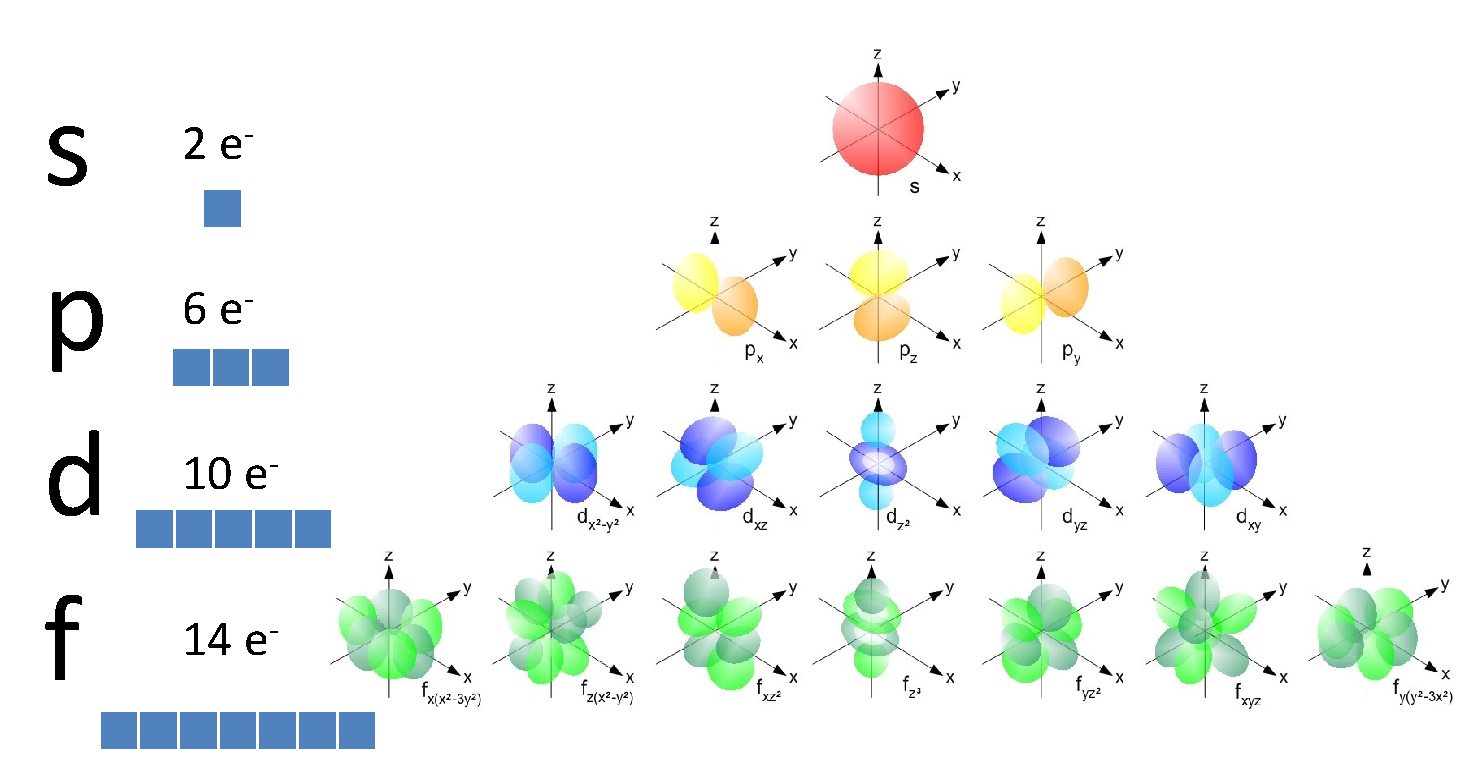
\includegraphics[width=\linewidth,height=52mm,keepaspectratio]{obrazky/emv1_p1_s13.pdf}
\par\vspace{1mm}{\scriptsize\sffamily\color{muted} Tvary a kapacity orbitalů s, p, d, f. P1, s. 13.\par}
\end{minipage}
\par\end{minipage}\par\vspace{6mm}
\noindent\begin{minipage}[b]{\linewidth}
\section*{2. Vysvětlete pravidla podle kterých se obsazuje (vystavuje) atomový obal elektrony}
\begin{enumerate}
\item \textbf{Princip minimální energie:} elektrony nejprve obsazují stavy s nejnižší energií.
\item \textbf{Pravidlo $n+l$:} dříve se zaplňuje podslupka s menším součtem $n+l$; při shodě s menším $n$. Pořadí: $1s,2s,2p,3s,3p,4s,3d,4p,\ldots$
\item \textbf{Pauliho princip:} dva elektrony v atomu nemohou mít všechna čtyři kvantová čísla shodná; jeden orbital pojme nejvýše dva elektrony s opačnými spiny.
\item \textbf{Hundovo pravidlo:} orbitaly téže energie se nejprve obsazují jednotlivě se souhlasnými spiny, teprve potom se elektrony párují.
\end{enumerate}

\par\vspace{2mm}
\begin{minipage}[t]{.94\linewidth}\centering
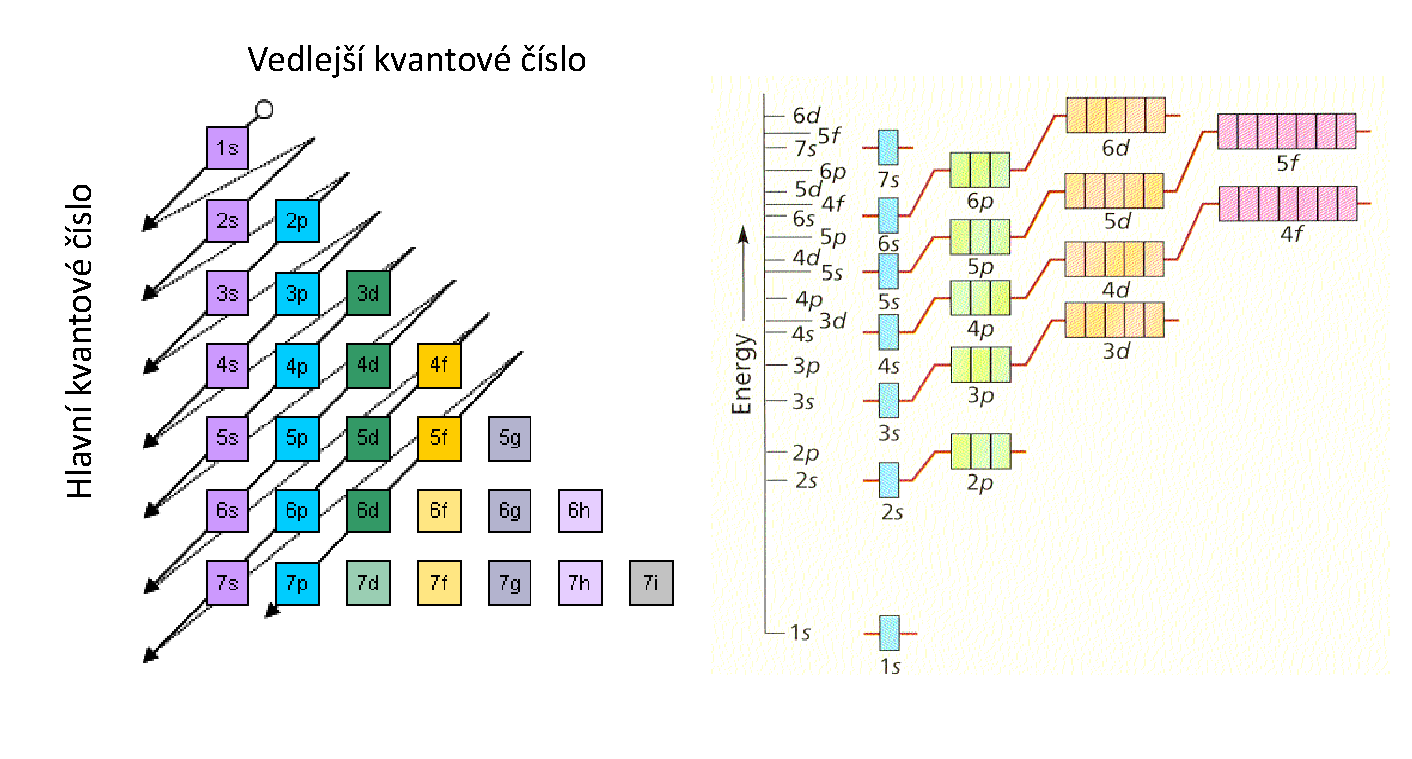
\includegraphics[width=\linewidth,height=52mm,keepaspectratio]{obrazky/emv1_p1_s15.pdf}
\par\vspace{1mm}{\scriptsize\sffamily\color{muted} Pořadí obsazování podslupek a energetické hladiny. P1, s. 15.\par}
\end{minipage}
\par\end{minipage}\par\vspace{6mm}
\noindent\begin{minipage}[b]{\linewidth}
\section*{3. Popište tři základní typy vazeb, která veličina má rozhodující vliv na povahu vazby?}
\begin{itemize}
\item \textbf{Kovová vazba:} kladné iontové zbytky spojují společné, volně pohyblivé valenční elektrony.
\item \textbf{Iontová vazba:} přenosem elektronu vznikne kationt a aniont, které se elektrostaticky přitahují; např. NaCl.
\item \textbf{Kovalentní vazba:} atomy sdílejí elektronové páry; při nerovnoměrném sdílení je vazba polární.
\end{itemize}
Rozhodující je \textbf{elektronegativita a její rozdíl $\Delta\chi$}: orientačně $\Delta\chi<0{,}4$ nepolární kovalentní, $0{,}4$--$1{,}7$ polární kovalentní a $>1{,}7$ iontová vazba. Kovová vazba vzniká mezi atomy kovů s nízkou elektronegativitou.

\par\vspace{2mm}
\begin{minipage}[t]{.48\linewidth}\centering
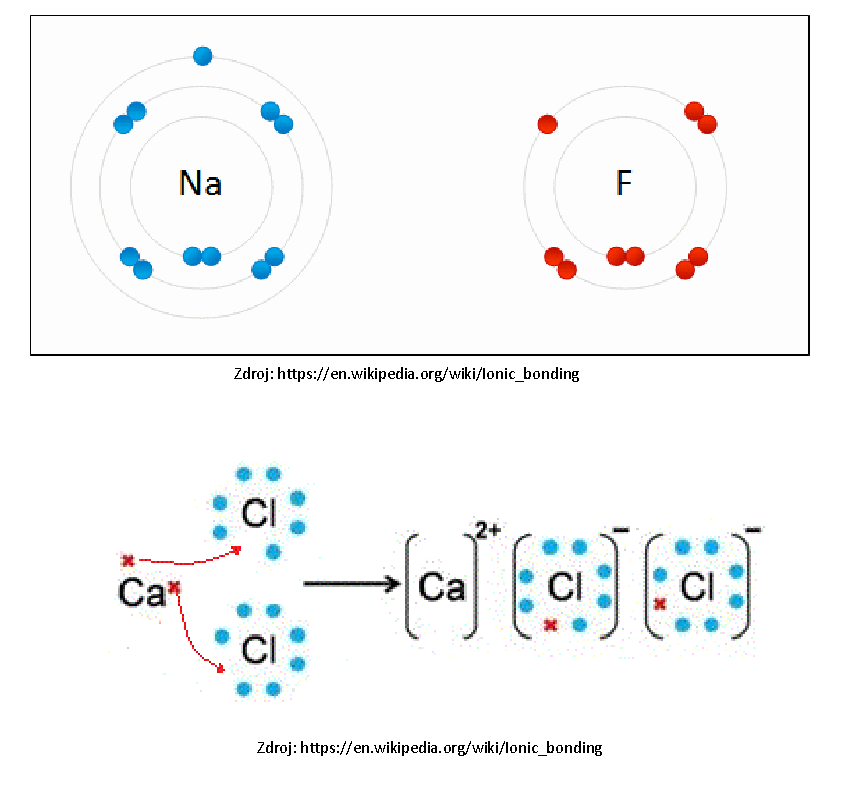
\includegraphics[width=\linewidth,height=52mm,keepaspectratio]{obrazky/emv1_p1_s26.pdf}
\par\vspace{1mm}{\scriptsize\sffamily\color{muted} Vznik iontové vazby přenosem elektronů. P1, s. 26.\par}
\end{minipage}\hfill
\begin{minipage}[t]{.48\linewidth}\centering
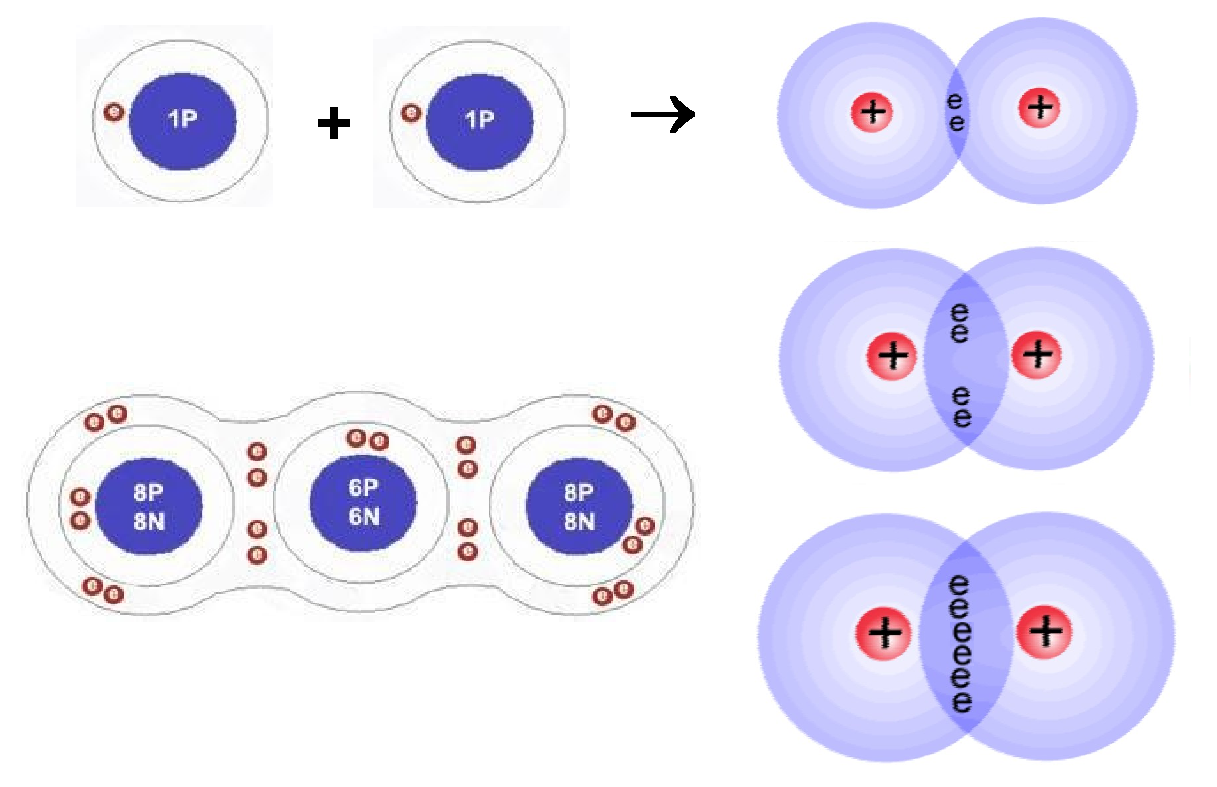
\includegraphics[width=\linewidth,height=52mm,keepaspectratio]{obrazky/emv1_p1_s30.pdf}
\par\vspace{1mm}{\scriptsize\sffamily\color{muted} Sdílení elektronů v kovalentní vazbě. P1, s. 30.\par}
\end{minipage}
\par\end{minipage}\par\vspace{6mm}
\noindent\begin{minipage}[b]{\linewidth}
\section*{4. Vysvětlete pojmy - ionizační energie, elektronová afinita a elektronegativita.}
\begin{itemize}
\item \textbf{Ionizační energie:} energie nutná k odtržení nejslaběji vázaného elektronu, $\mathrm A\to\mathrm{A^+}+e^-$. První ionizační energie se vztahuje k neutrálnímu atomu, druhá k odtržení dalšího elektronu z kationtu.
\item \textbf{Elektronová afinita:} energie uvolněná při přijetí volného elektronu neutrálním atomem, $\mathrm A+e^-\to\mathrm{A^-}$.
\item \textbf{Elektronegativita:} schopnost atomu přitahovat elektrony v chemické vazbě.
\end{itemize}
Ionizační energie a afinita se udávají v eV na částici nebo kJ/mol; elektronegativita je bezrozměrná.

\par\end{minipage}\par\vspace{6mm}
\noindent\begin{minipage}[b]{\linewidth}
\section*{5. Vysvětlete proč molekula složená z prvků se silnou iontovou či kovalentní polární vazbou (např. molekula plynu fluoridu sírového - SF6) může být navenek nepolární.}
Polarita molekuly závisí na \textbf{vektorovém součtu dipólových momentů všech vazeb}:
\[\boldsymbol p_{\mathrm{mol}}=\sum_i\boldsymbol p_i.\]
V SF$_6$ jsou vazby S--F polární, ale šest atomů F tvoří pravidelný oktaedr. Protilehlé vazby mají stejně velké a opačné dipólové momenty, které se vyruší. Těžiště kladného a záporného náboje splývají, proto molekula nemá permanentní dipólový moment a je navenek nepolární.

\par\vspace{2mm}
\begin{minipage}[t]{.94\linewidth}\centering
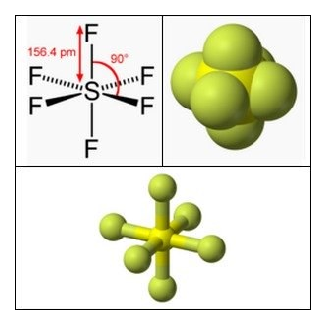
\includegraphics[width=\linewidth,height=52mm,keepaspectratio]{obrazky/emv1_p1_s39.pdf}
\par\vspace{1mm}{\scriptsize\sffamily\color{muted} Symetrické prostorové uspořádání SF6. P1, s. 39.\par}
\end{minipage}
\par\end{minipage}\par\vspace{6mm}
\noindent\begin{minipage}[b]{\linewidth}
\section*{6. Co je to polarizace? Popište čtyři vybrané typy polarizačních mechanismů a seřaďte je podle jejich rychlosti.}
\textbf{Polarizace} je posun vázaných nábojů, orientace dipólů nebo hromadění nábojů na nehomogenitách působením elektrického pole. Čtyři mechanismy od nejrychlejšího:
\begin{enumerate}
\item \textbf{Elektronová:} posun elektronového obalu vůči jádru, $10^{-16}$--$10^{-14}$ s.
\item \textbf{Iontová pružná:} vzájemný posun kladných a záporných iontů v mřížce, $10^{-13}$--$10^{-12}$ s.
\item \textbf{Dipólová orientační:} natáčení permanentních dipólů do směru pole; u nízkomolekulárních látek $10^{-12}$--$10^{-8}$ s.
\item \textbf{Mezivrstvová:} nahromadění pohyblivých nábojů na rozhraních nehomogenit; z uvedených nejpomalejší.
\end{enumerate}

\par\vspace{2mm}
\begin{minipage}[t]{.94\linewidth}\centering
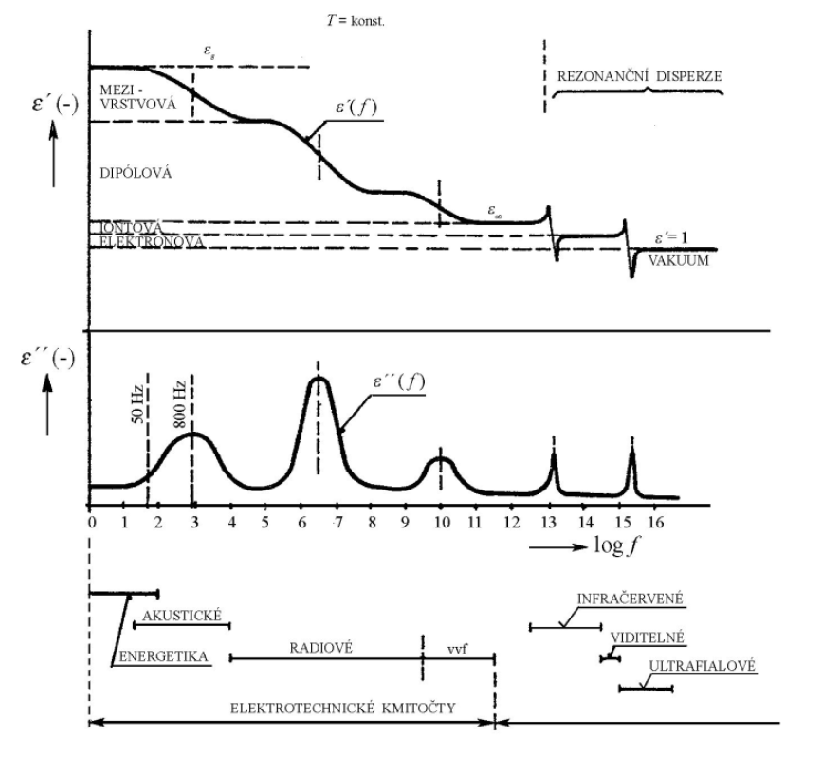
\includegraphics[width=\linewidth,height=52mm,keepaspectratio]{obrazky/emv1_p2_s36.pdf}
\par\vspace{1mm}{\scriptsize\sffamily\color{muted} Frekvenční oblasti polarizačních mechanismů. P2, s. 36.\par}
\end{minipage}
\par\end{minipage}\par\vspace{6mm}
\noindent\begin{minipage}[b]{\linewidth}
\section*{7. Načtrtněte a popište mezivrstvou polarizaci.}
\textbf{Mezivrstvová polarizace} vzniká v nehomogenním dielektriku hromaděním pohyblivých nábojů na rozhraních oblastí s odlišnými elektrickými vlastnostmi. Přiložené pole oddělí náboje, které se na nehomogenitách zachytí a vytvářejí prostorové dipóly. Jde o pomalý polarizační mechanismus; oddělení nábojů znázorňuje schéma.

\par\vspace{2mm}
\begin{minipage}[t]{.94\linewidth}\centering
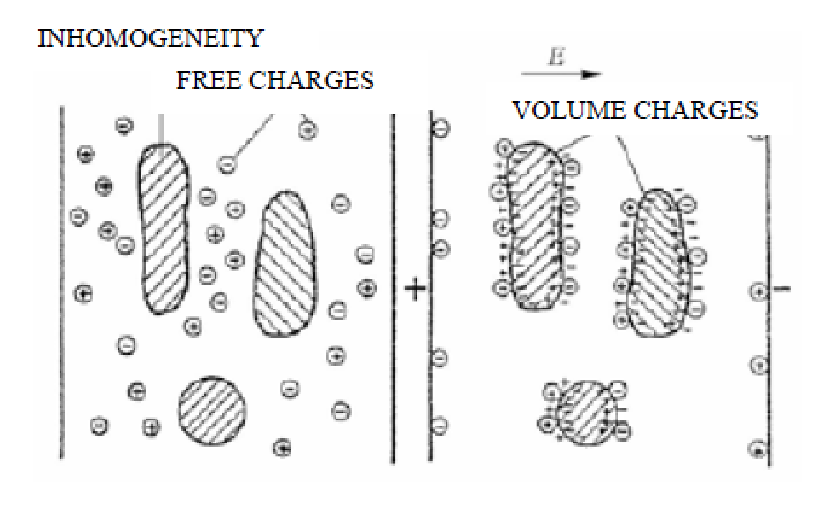
\includegraphics[width=\linewidth,height=52mm,keepaspectratio]{obrazky/emv1_p1_s46.pdf}
\par\vspace{1mm}{\scriptsize\sffamily\color{muted} Hromadění nábojů na nehomogenitách po přiložení pole. P1, s. 46.\par}
\end{minipage}
\par\end{minipage}\par\vspace{6mm}
\noindent\begin{minipage}[b]{\linewidth}
\section*{8. Jaké veličiny popisují dielektrické materiály a jaké mají jednotky?}
\begin{itemize}
\item \textbf{Permitivita} $\varepsilon$ [F/m]; \textbf{relativní permitivita} $\varepsilon_r=\varepsilon/\varepsilon_0$ [1].
\item \textbf{Komplexní relativní permitivita} $\varepsilon_r^*=\varepsilon'-j\varepsilon''$ [1]; $\varepsilon'$ je reálná složka, $\varepsilon''$ \textbf{ztrátové číslo} [1].
\item \textbf{Ztrátový úhel} $\delta$ [rad] a \textbf{ztrátový činitel} $\tan\delta=\varepsilon''/\varepsilon'$ [1].
\item \textbf{Vnitřní (objemová) rezistivita} $\rho_V$ [$\Omega$\,m] a \textbf{povrchová rezistivita} $\rho_S$ [$\Omega$].
\item \textbf{Elektrická pevnost} $E_p$ [V/m, běžně kV/mm]: mezní intenzita pole před průrazem.
\end{itemize}

\par\end{minipage}\par\vspace{6mm}
\noindent\begin{minipage}[b]{\linewidth}
\section*{9. Jaké jsou typické hodnoty relativní permitivity pro epoxidovou pryskyřici, Polypropylen, PTFE, vodu, slídu, sklo a titaničitatan barnatý?}
Relativní permitivita $\varepsilon_r$ je bezrozměrná. Hodnoty uvedené v prezentacích:
\begin{center}\begin{tabular}{lr}
Epoxidová pryskyřice & $3{,}6$\\
Polypropylen & $2{,}2$\\
PTFE & $2{,}1$\\
Voda při $20\,^{\circ}\mathrm C$ & $81$\\
Slída & $6{,}9$--$11{,}5$\\
Sklo & $3{,}8$--$19$\\
Keramika na bázi BaTiO$_3$ & $500$--$15\,000$
\end{tabular}\end{center}
Prvních šest hodnot je z tabulky pro 100 Hz; rozsah pro BaTiO$_3$ je uveden u vysokodielektrické keramiky.

\par\end{minipage}\par\vspace{6mm}
\noindent\begin{minipage}[b]{\linewidth}
\section*{10. Co vyjadřuje Clausiova-Mossotiho rovnice?}
Clausiova--Mossottiho rovnice spojuje \textbf{makroskopickou relativní permitivitu} s \textbf{koncentrací a polarizovatelností částic}:
\[\boxed{\frac{\varepsilon_r-1}{\varepsilon_r+2}=\frac{n\alpha}{3\varepsilon_0}}.\]
$n$ je počet částic v jednotce objemu, $\alpha$ polarizovatelnost jedné částice a $\varepsilon_0$ permitivita vakua.

\par\vspace{2mm}
\begin{minipage}[t]{.94\linewidth}\centering
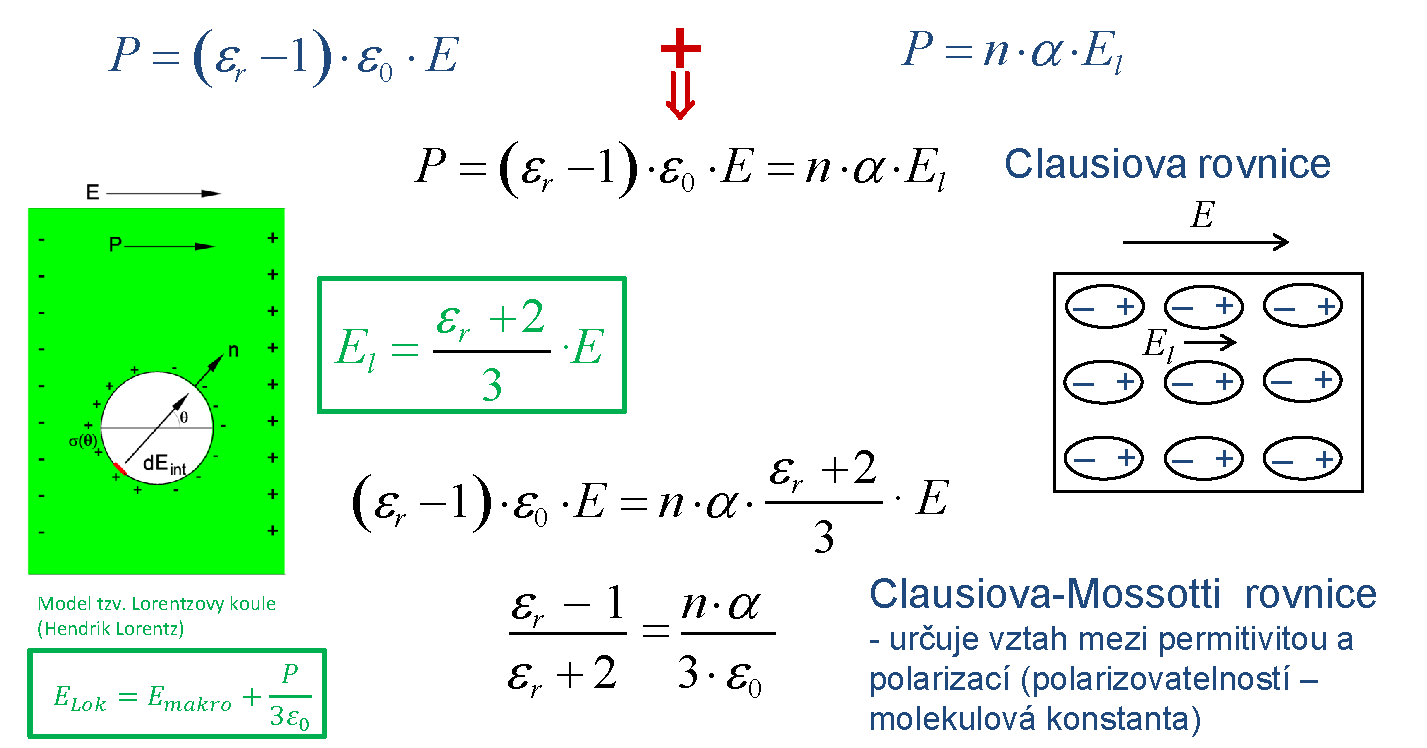
\includegraphics[width=\linewidth,height=52mm,keepaspectratio]{obrazky/emv1_p2_s09.pdf}
\par\vspace{1mm}{\scriptsize\sffamily\color{muted} Lokální pole a vztah mezi permitivitou a polarizovatelností. P2, s. 9.\par}
\end{minipage}
\par\end{minipage}\par\vspace{6mm}
\noindent\begin{minipage}[b]{\linewidth}
\section*{11. Napište Debayeovu rovnici a vysvětlete jednotlivé veličiny.}
Debyeova rovnice pro jeden polarizační mechanismus s jedinou relaxační dobou:
\[\boxed{\varepsilon_r^*(\omega)=\varepsilon_\infty+\frac{\varepsilon_s-\varepsilon_\infty}{1+j\omega\tau}=\varepsilon'-j\varepsilon''}.\]
\begin{itemize}
\item $\varepsilon_r^*$: komplexní relativní permitivita; $\varepsilon'$ její reálná složka a $\varepsilon''$ ztrátové číslo.
\item $\varepsilon_s$: statická relativní permitivita ($f\to0$); $\varepsilon_\infty$: vysokofrekvenční mez ($f\to\infty$).
\item $\tau$ [s]: relaxační doba polarizačního mechanismu.
\item $\omega=2\pi f$ [rad/s]: úhlová frekvence, $f$ [Hz]: frekvence; $j$ je imaginární jednotka, $j^2=-1$.
\end{itemize}

\par\end{minipage}\par\vspace{6mm}
\noindent\begin{minipage}[b]{\linewidth}
\section*{12. Načrtněte a popište frekvenční závislost relativní permitivity, ztrátového čísla a ztrátového činitele v případě jednoho polarizačního mechanismu. Vyznačte bod mezní frekvence a napište jak souvisí s relaxační dobou daného polarizačního mechanismu.}
Při zvyšování frekvence u jednoho relaxačního mechanismu:
\begin{itemize}
\item \textbf{Relativní permitivita $\varepsilon'$} klesá ze statické hodnoty $\varepsilon_s$ k vysokofrekvenční mezi $\varepsilon_\infty$, protože dipóly přestávají sledovat změny pole.
\item \textbf{Ztrátové číslo $\varepsilon''$} roste do maxima při mezní frekvenci $f_m$ a potom klesá.
\item \textbf{Ztrátový činitel $\tan\delta=\varepsilon''/\varepsilon'$} má rovněž relaxační maximum a při velmi nízkých i vysokých frekvencích klesá.
\end{itemize}
Mezní frekvenci vyznačuje přerušovaná čára v grafu; s relaxační dobou souvisí vztahem
\[\boxed{f_m=\frac{1}{2\pi\tau}},\qquad\omega_m\tau=1.\]

\par\vspace{2mm}
\begin{minipage}[t]{.94\linewidth}\centering
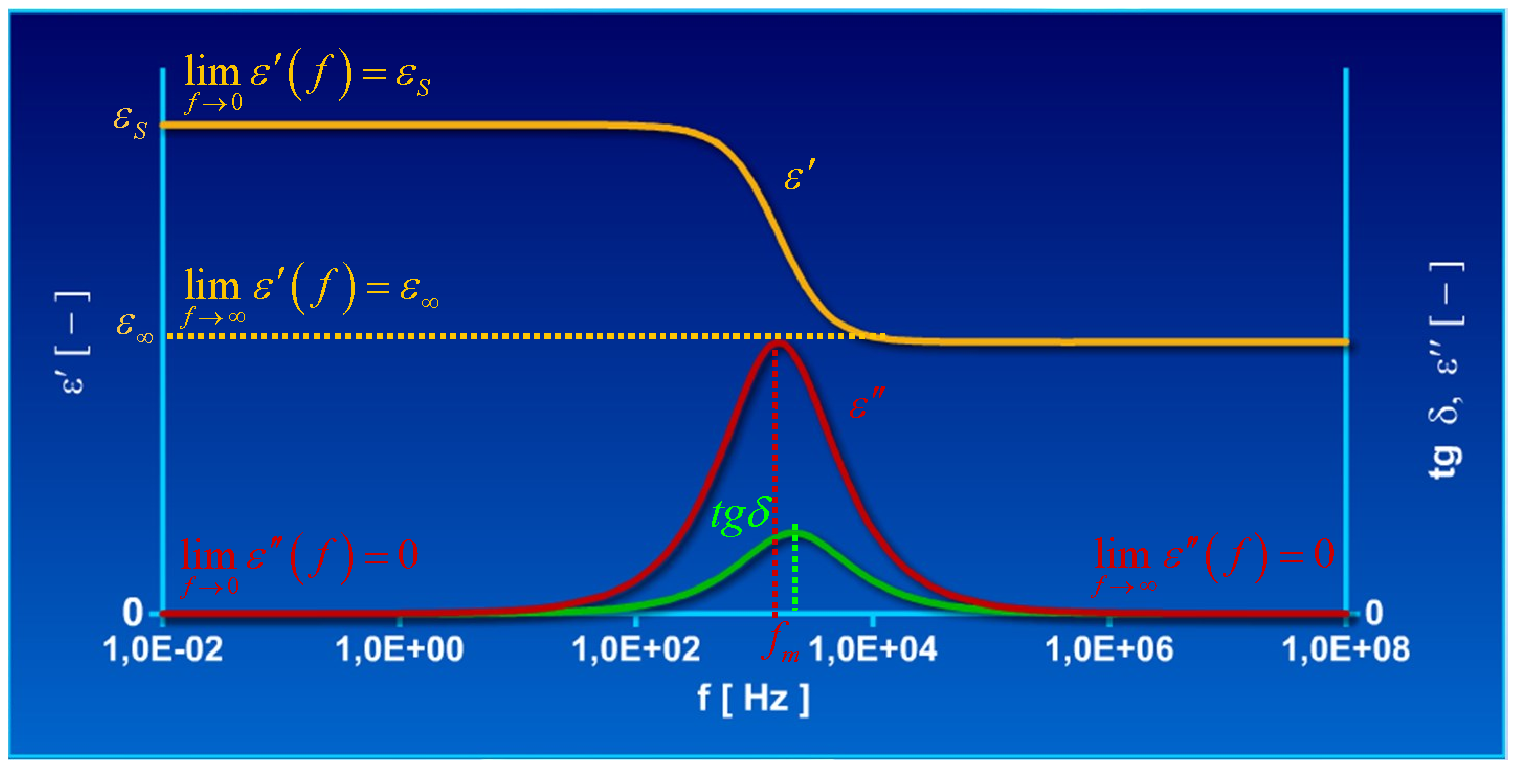
\includegraphics[width=\linewidth,height=52mm,keepaspectratio]{obrazky/emv1_p2_s20.pdf}
\par\vspace{1mm}{\scriptsize\sffamily\color{muted} Permitivita, ztrátové číslo a ztrátový činitel jedné relaxace. P2, s. 20.\par}
\end{minipage}
\par\end{minipage}\par\vspace{6mm}
\noindent\begin{minipage}[b]{\linewidth}
\section*{13. Jak se od sebe liší Cole-Coleho a Havriliak-Negamiho diagram a který lépe reprezentuje reálné dielektrikum a proč.}
Diagramy zobrazují ztrátové číslo $\varepsilon''$ proti reálné složce permitivity $\varepsilon'$; frekvence je parametr.
\begin{itemize}
\item \textbf{Cole--Cole:} kruhový oblouk odpovídající symetrickému rozdělení relaxačních dob; při rozšíření rozdělení leží střed kružnice pod reálnou osou. Debyeův případ s jedinou relaxační dobou je půlkružnice se středem na ose.
\item \textbf{Havriliak--Negami:} umožňuje kromě rozšíření i asymetrii rozdělení relaxačních dob, tedy nesymetrický oblouk.
\end{itemize}
\textbf{Havriliakův--Negamiho model lépe vystihuje reálné dielektrikum}, protože jeho polarizující částice nemají jedinou relaxační dobu a jejich rozdělení může být nesymetrické.

\par\vspace{2mm}
\begin{minipage}[t]{.48\linewidth}\centering
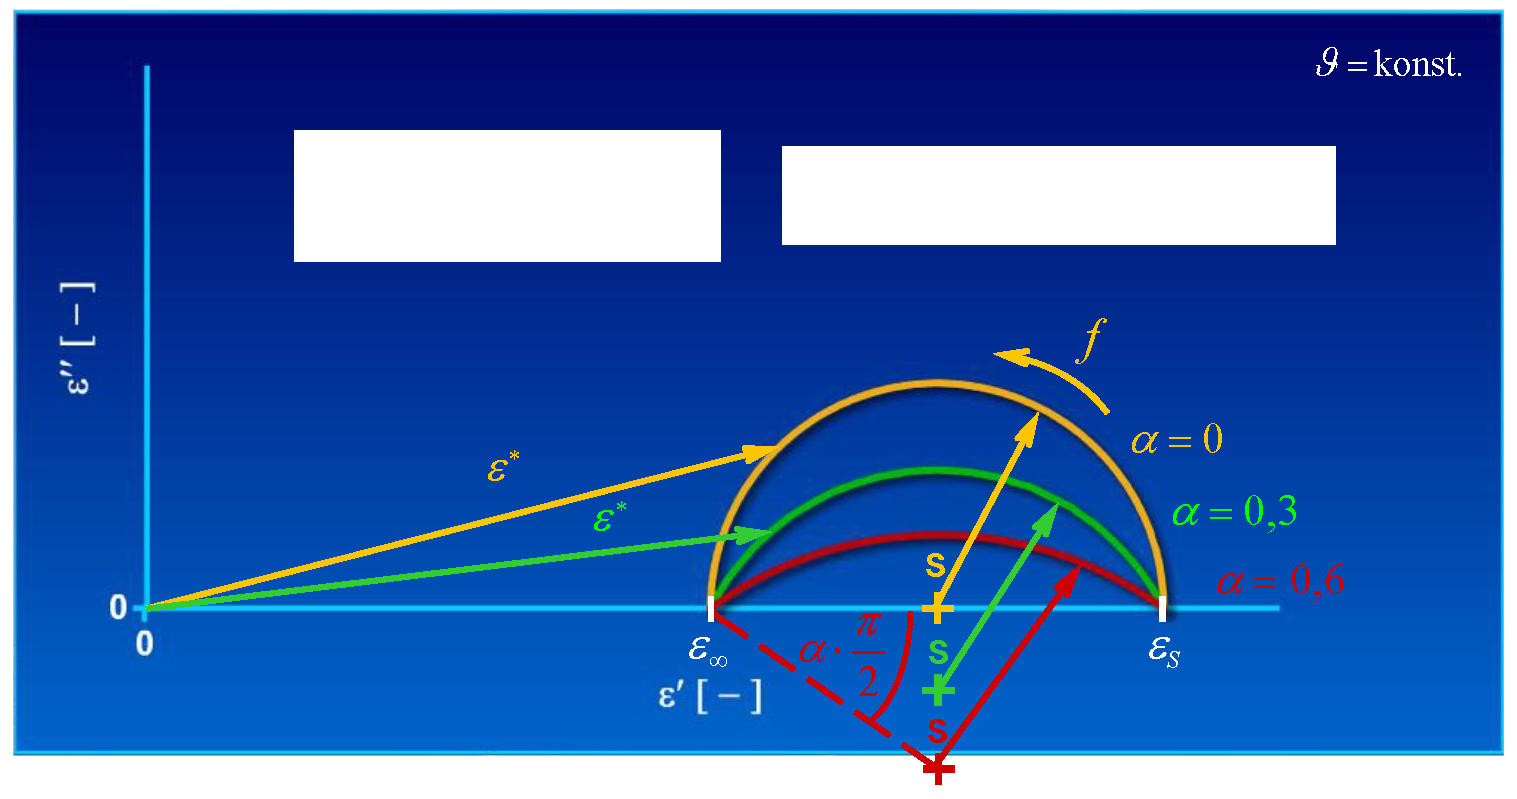
\includegraphics[width=\linewidth,height=52mm,keepaspectratio]{obrazky/emv1_p2_s29.pdf}
\par\vspace{1mm}{\scriptsize\sffamily\color{muted} Vliv šířky rozdělení relaxačních dob. P2, s. 29.\par}
\end{minipage}\hfill
\begin{minipage}[t]{.48\linewidth}\centering
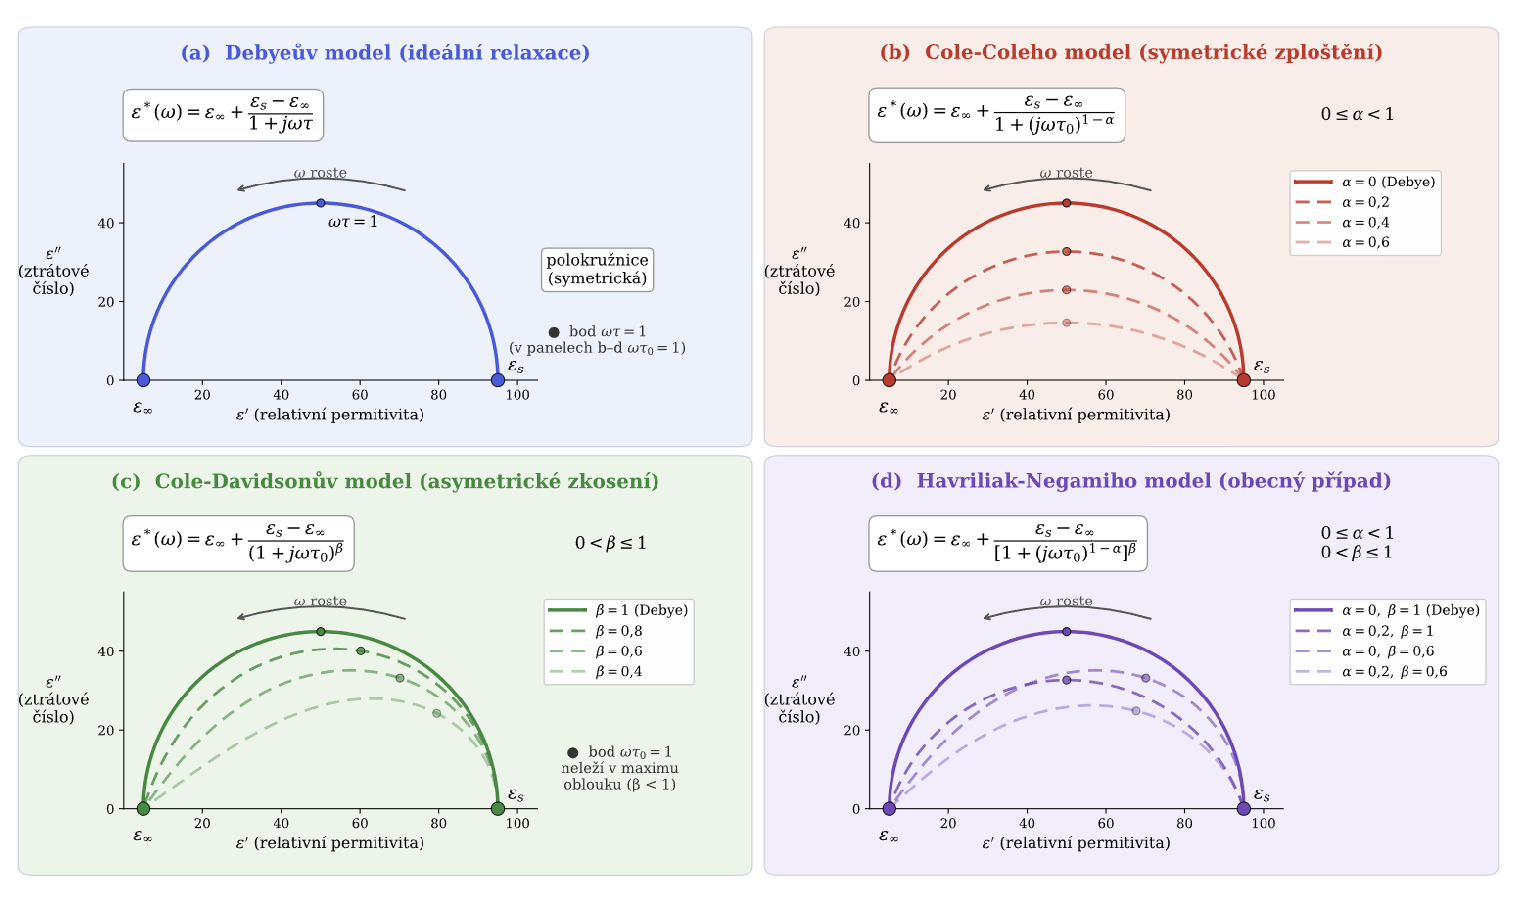
\includegraphics[width=\linewidth,height=52mm,keepaspectratio]{obrazky/emv1_p2_s33.pdf}
\par\vspace{1mm}{\scriptsize\sffamily\color{muted} Porovnání Debyeova, Coleových a HN modelu. P2, s. 33.\par}
\end{minipage}
\par\end{minipage}\par\vspace{6mm}
\noindent\begin{minipage}[b]{\linewidth}
\section*{14. Jaké jsou příčiny ztrát v dielektriku a jaké máme kategorie?}
Dielektrické ztráty jsou přeměnou elektrické energie na teplo. Podle příčiny se dělí na:
\begin{itemize}
\item \textbf{Vodivostní:} pohyb volných nosičů náboje v objemu nebo po povrchu izolantu; vznikají při stejnosměrném i střídavém poli.
\item \textbf{Polarizační:} zpoždění relaxační polarizace za změnami pole; energie se spotřebovává při přemisťování iontů nebo natáčení dipólů.
\item \textbf{Ionizační:} ionizace plynu a výboje, např. v plynových dutinách izolantu při dostatečně silném poli.
\end{itemize}

\par\vspace{2mm}
\begin{minipage}[t]{.94\linewidth}\centering
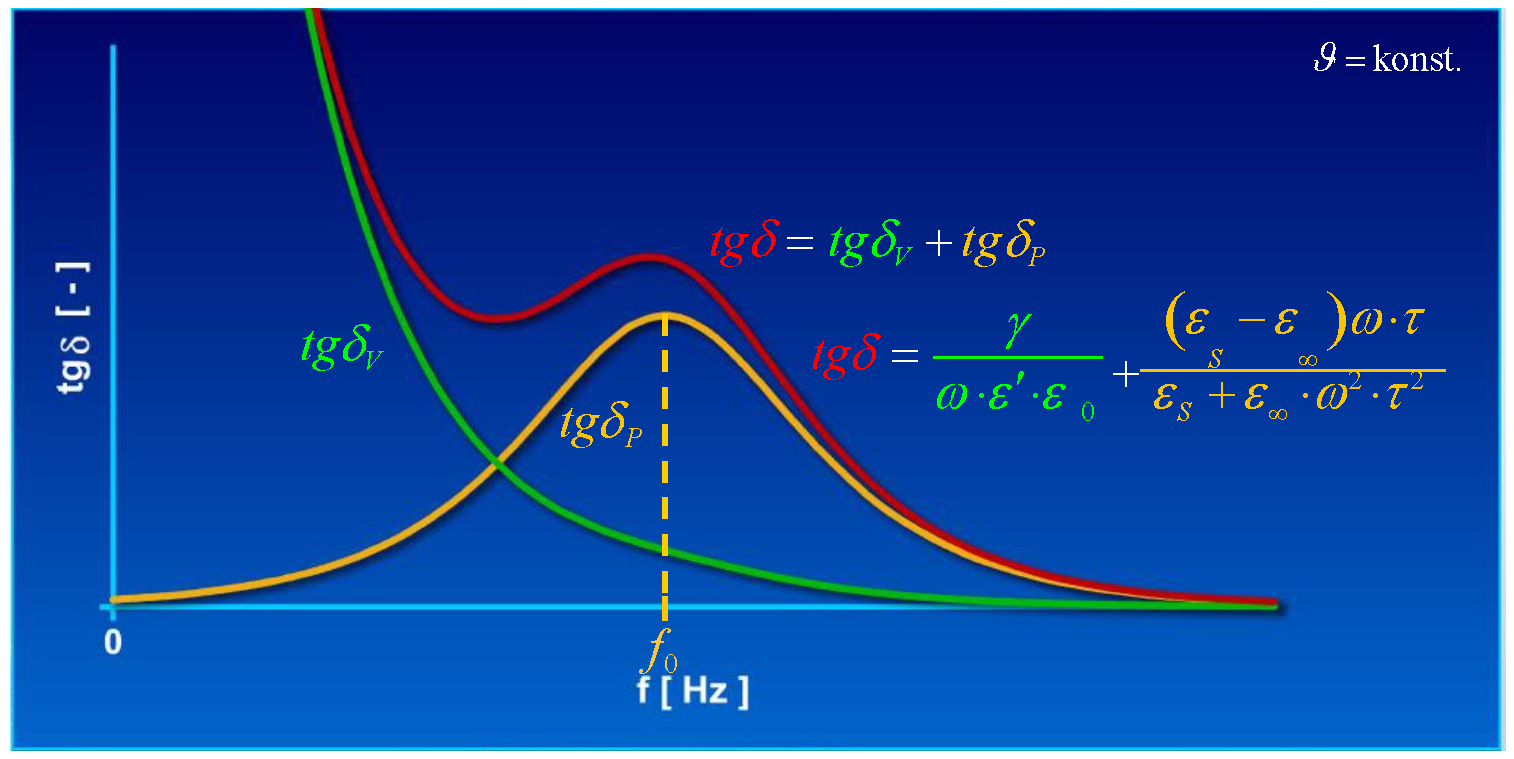
\includegraphics[width=\linewidth,height=52mm,keepaspectratio]{obrazky/emv1_p2_s53.pdf}
\par\vspace{1mm}{\scriptsize\sffamily\color{muted} Součet vodivostního a polarizačního příspěvku. P2, s. 53.\par}
\end{minipage}
\par\end{minipage}\par\vspace{6mm}
\noindent\begin{minipage}[b]{\linewidth}
\section*{15. Jaký je vliv teploty na frekvenční závislost celkových ztrát v polárním dielektriku?}
S růstem teploty se mění oba příspěvky celkových ztrát:
\begin{itemize}
\item \textbf{Polarizační:} relaxační doba $\tau$ klesá a maximum se posouvá k \textbf{vyšším frekvencím}, protože $f_m=1/(2\pi\tau)$.
\item \textbf{Vodivostní:} konduktivita roste, a proto se zvyšuje nízkofrekvenční větev ztrátového činitele.
\end{itemize}
Celkový průběh je součtem vodivostního a polarizačního příspěvku.

\par\vspace{2mm}
\begin{minipage}[t]{.94\linewidth}\centering
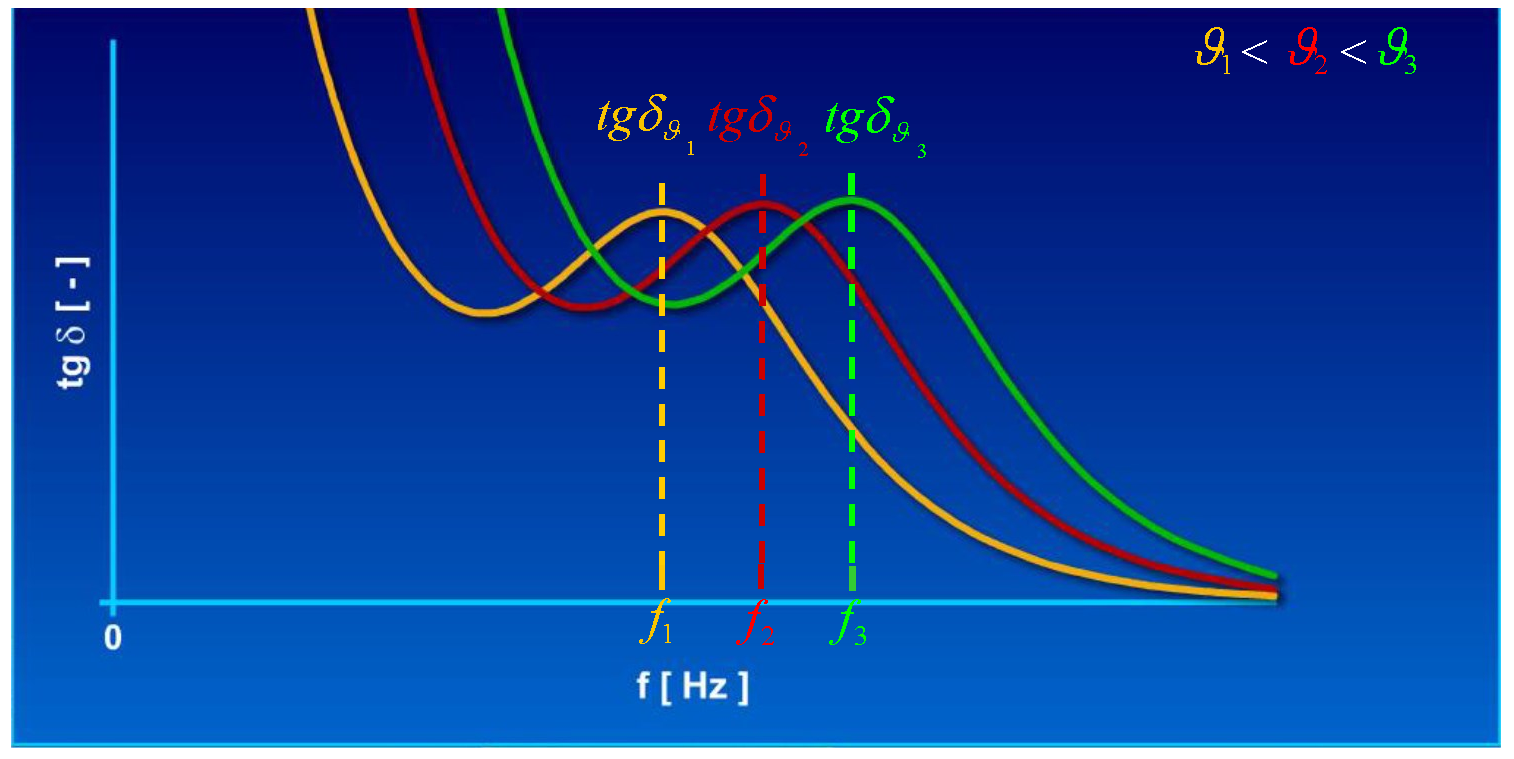
\includegraphics[width=\linewidth,height=52mm,keepaspectratio]{obrazky/emv1_p2_s54.pdf}
\par\vspace{1mm}{\scriptsize\sffamily\color{muted} Posun relaxačních maxim při růstu teploty. P2, s. 54.\par}
\end{minipage}
\par\end{minipage}\par\vspace{6mm}
\noindent\begin{minipage}[b]{\linewidth}
\section*{16. Vysvětlete na jakých veličinách závisí konduktivita materiálu a jak ovlivňuje vodivostní ztráty.}
Konduktivita závisí na \textbf{koncentraci, náboji a pohyblivosti nosičů}:
\[\boxed{\sigma=n|q|\mu}\quad[\mathrm{S/m}].\]
$n$ [m$^{-3}$] je koncentrace nosičů, $|q|$ [C] velikost jejich náboje a $\mu$ [m$^2$/(V\,s)] pohyblivost. Větší koncentrace nebo pohyblivost znamená větší konduktivitu.

Vodivostní složka ztrátového činitele je
\[\tan\delta_{\mathrm{vod}}=\frac{\sigma}{\omega\varepsilon_0\varepsilon'},\qquad\omega=2\pi f.\]
Při ostatních parametrech stejných tedy vodivostní ztráty rostou s konduktivitou a jejich ztrátový činitel klesá s frekvencí jako $1/f$.

\par\end{minipage}\par\vspace{6mm}
\noindent\begin{minipage}[b]{\linewidth}
\section*{17. Načrtněte a popište model dvojité potenciálové jámy bez a s přítomností elektrického pole. Jak se liší pravděpodobnosti přeskoku? K čemu je tento model používán?}
Dvě potenciálová minima představují možné polohy iontu, oddělené energetickou bariérou $W$.
\begin{itemize}
\item \textbf{Bez pole:} obě polohy jsou rovnocenné. Pravděpodobnosti přeskoku v obou směrech jsou stejné a jsou úměrné $e^{-W/(k_BT)}$; nevzniká usměrněný pohyb.
\item \textbf{S polem:} pro kladný iont se bariéra ve směru pole sníží na $W-\Delta W$, proti poli zvýší na $W+\Delta W$. Přeskok ve směru pole je pravděpodobnější, vzniká usměrněný pohyb iontů.
\end{itemize}
$k_B$ je Boltzmannova konstanta a $T$ absolutní teplota. Model slouží k vysvětlení \textbf{tepelně aktivované iontové vodivosti a iontové relaxační polarizace}.

\par\vspace{2mm}
\begin{minipage}[t]{.48\linewidth}\centering
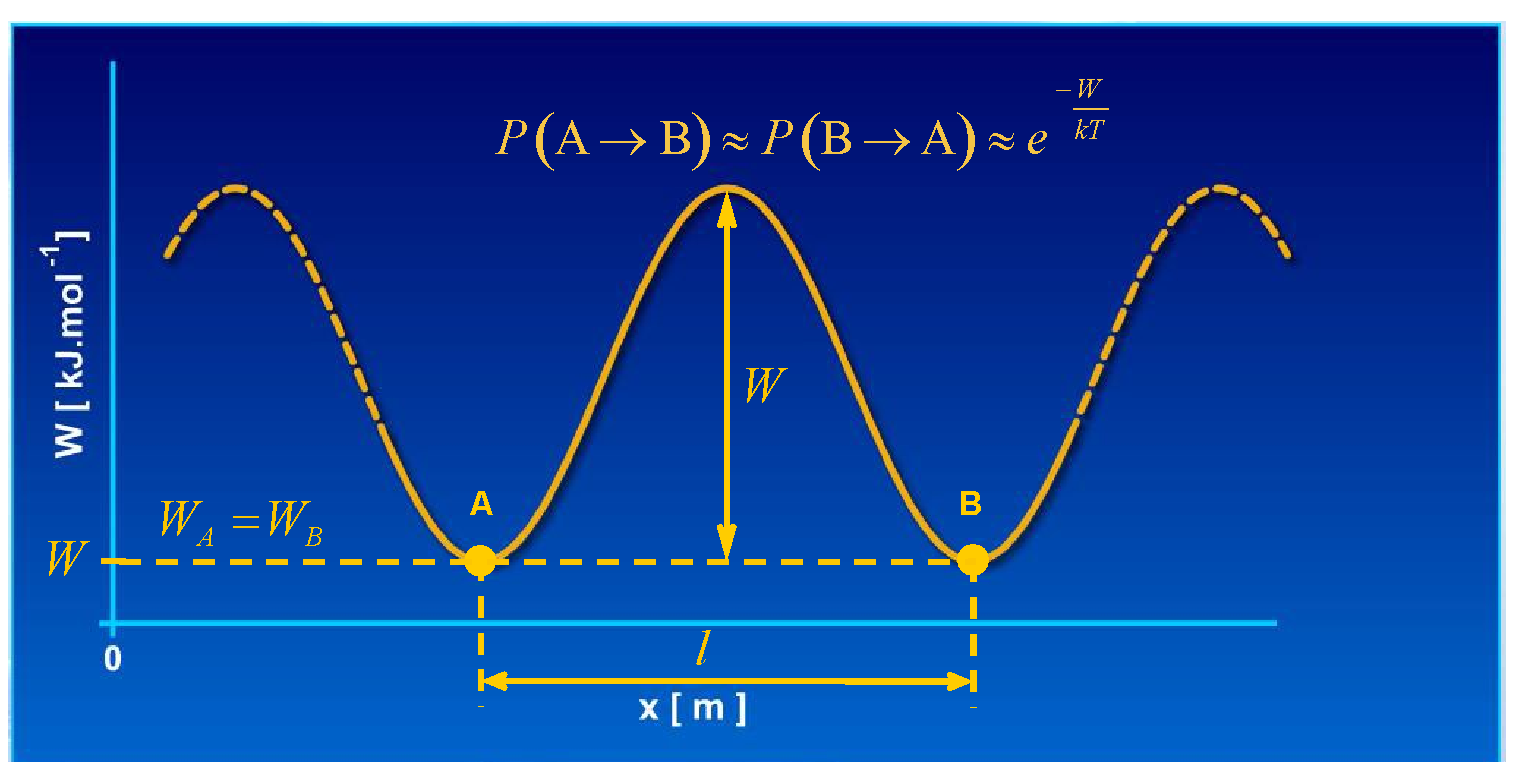
\includegraphics[width=\linewidth,height=52mm,keepaspectratio]{obrazky/emv1_p3_s21.pdf}
\par\vspace{1mm}{\scriptsize\sffamily\color{muted} Dvě rovnocenné polohy bez vnějšího pole. P3, s. 21.\par}
\end{minipage}\hfill
\begin{minipage}[t]{.48\linewidth}\centering
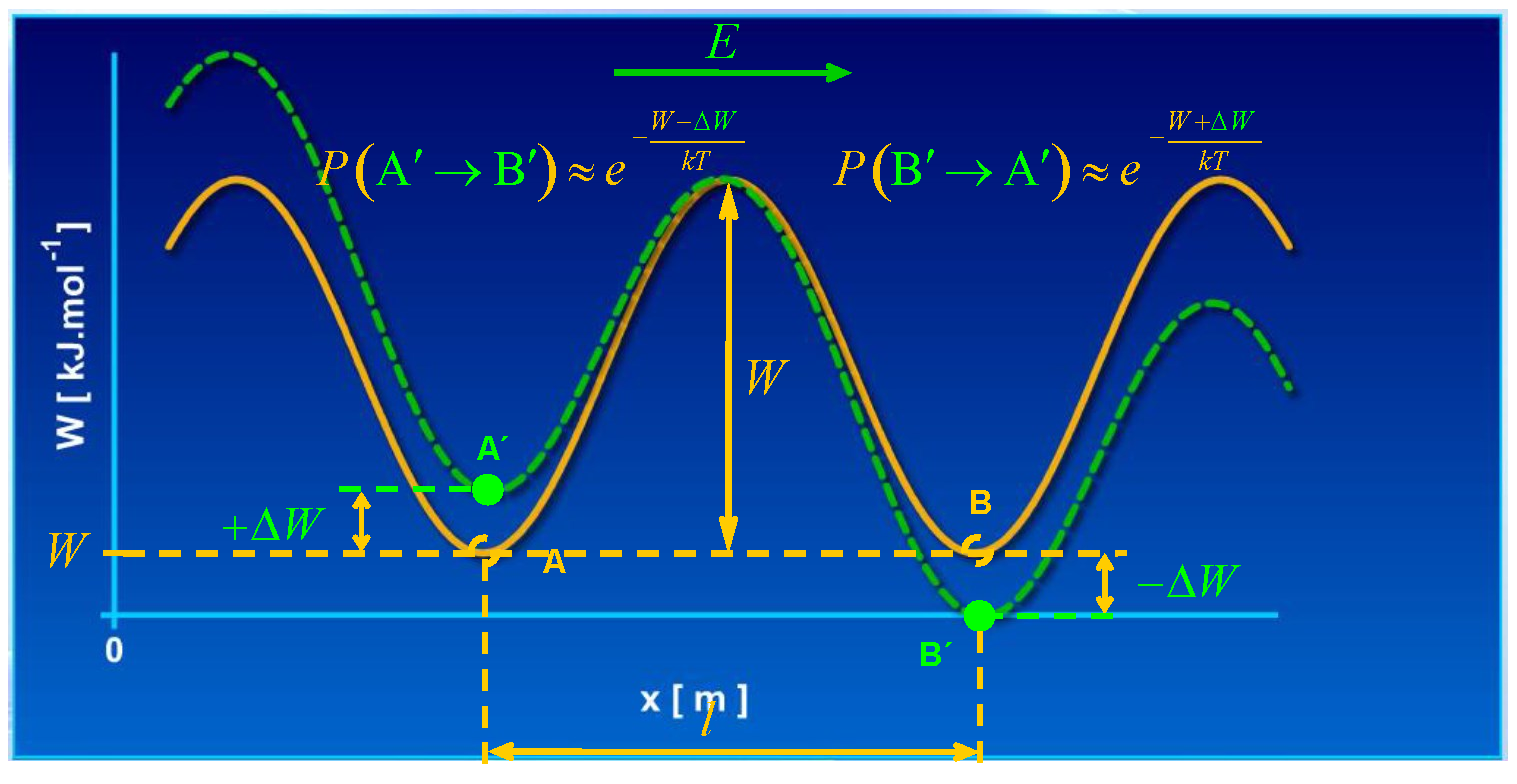
\includegraphics[width=\linewidth,height=52mm,keepaspectratio]{obrazky/emv1_p3_s23.pdf}
\par\vspace{1mm}{\scriptsize\sffamily\color{muted} Elektrické pole sníží bariéru ve směru driftu. P3, s. 23.\par}
\end{minipage}
\par\end{minipage}\par\vspace{6mm}
\noindent\begin{minipage}[b]{\linewidth}
\section*{18. Popište mechanismy vodivosti u elektroizolačních kapalin, iontových krystalů a sklených amorfních látek, co je to vlastní a nevlastní vodivost kapalin?}
\begin{itemize}
\item \textbf{Elektroizolační kapaliny:} proud přenášejí ionty. \emph{Vlastní vodivost} vzniká disociací molekul samotné kapaliny, \emph{nevlastní} disociací nečistot a příměsí, např. vody. Pohyb nabitých koloidních částic způsobuje elektroforetickou vodivost.
\item \textbf{Iontové krystaly:} vodivost umožňují poruchy mřížky a přeskoky iontů mezi polohami. Schottkyho porucha vytváří vakance, Frenkelova vakanci a iont v mezimřížkové poloze.
\item \textbf{Skelné amorfní látky:} vodivost je iontová; v nepravidelné síti se pohybují zejména slabě vázané alkalické ionty Na$^+$ a K$^+$. Konduktivita závisí na jejich obsahu a pohyblivosti.
\end{itemize}

\par\vspace{2mm}
\begin{minipage}[t]{.94\linewidth}\centering
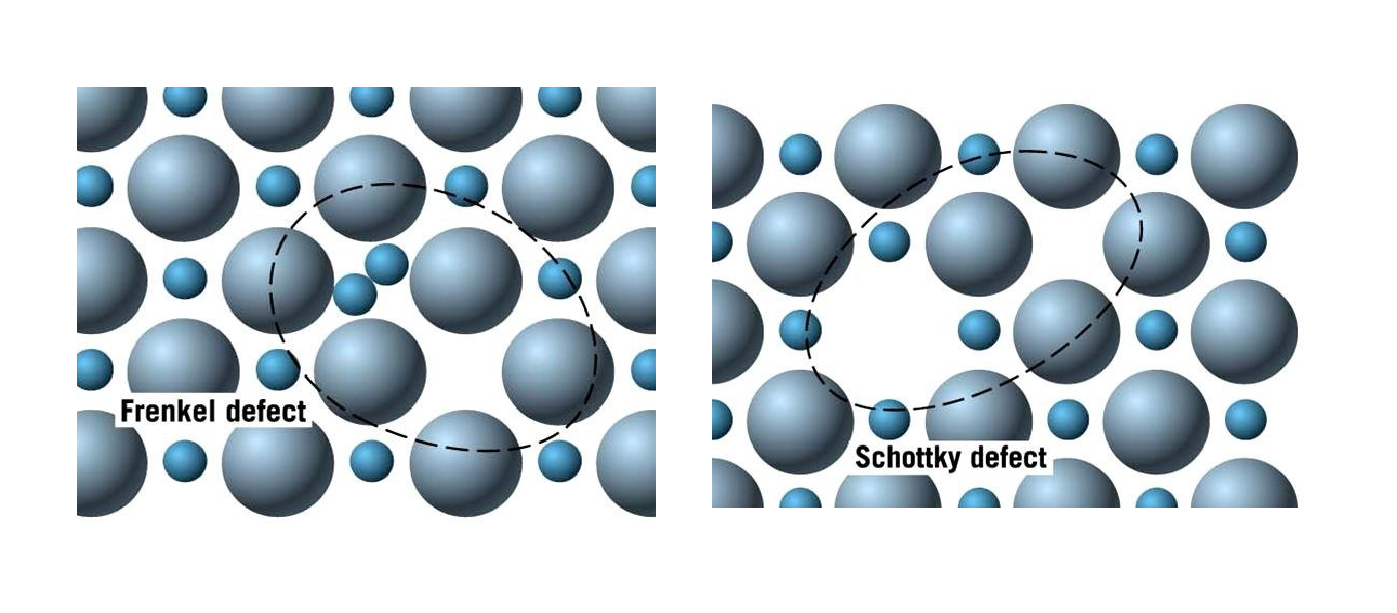
\includegraphics[width=\linewidth,height=52mm,keepaspectratio]{obrazky/emv1_p3_s30.pdf}
\par\vspace{1mm}{\scriptsize\sffamily\color{muted} Frenkelova a Schottkyho porucha krystalové mřížky. P3, s. 30.\par}
\end{minipage}
\par\end{minipage}\par\vspace{6mm}
\noindent\begin{minipage}[b]{\linewidth}
\section*{19. Čím je dána teplotní závislost vodivost u kapalných a u pevných látek?}
Protože $\sigma=n|q|\mu$, teplota ovlivňuje vodivost změnou koncentrace nosičů $n$ a jejich pohyblivosti $\mu$.
\begin{itemize}
\item \textbf{Kapalné izolanty:} rozhodující je změna pohyblivosti iontů. S teplotou klesá viskozita $\eta$, takže roste $\mu$ i vodivost; při neměnné koncentraci platí přibližně $\sigma\eta=\mathrm{konst.}$
\item \textbf{Pevné izolanty:} rozhodující je teplotně podmíněné uvolňování nosičů a vznik poruch mřížky. Vyšší teplota usnadňuje překonání energetických bariér. Ve skle se navíc mění pohyblivost iontů podle viskozity skelné sítě.
\end{itemize}
V přednášce je závislost vyjádřena $\sigma=Ae^{-b/T}$, kde $A,b$ jsou materiálové konstanty: s teplotou konduktivita roste.

\par\vspace{2mm}
\begin{minipage}[t]{.94\linewidth}\centering
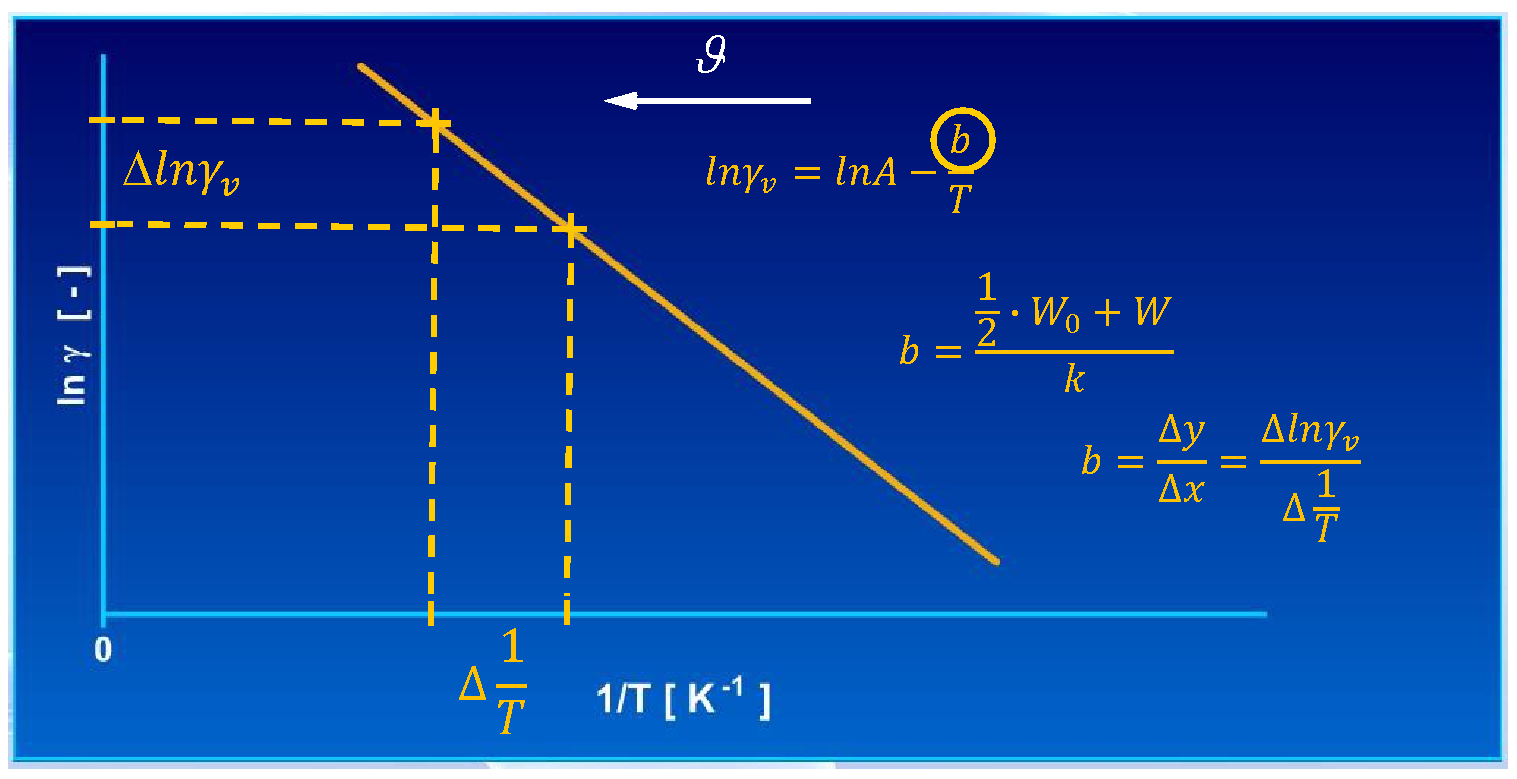
\includegraphics[width=\linewidth,height=52mm,keepaspectratio]{obrazky/emv1_p3_s34.pdf}
\par\vspace{1mm}{\scriptsize\sffamily\color{muted} Arrheniův graf; směrnice křivky je záporná. P3, s. 34.\par}
\end{minipage}
\par\end{minipage}\par\vspace{6mm}
\noindent\begin{minipage}[b]{\linewidth}
\section*{20. Co je to ionizace, jaké znáte druhy (zdroje) ionizace a jaké jsou podmínky vniku ionizace?}
\textbf{Ionizace} je vznik iontů; odtržením elektronu z neutrálního atomu vznikne kladný iont a volný elektron. Je třeba dodat alespoň ionizační energii $E_i$.
\begin{itemize}
\item \textbf{Nárazová ionizace:} srážka s částicí, jejíž kinetická energie splňuje $\tfrac12mv^2\ge E_i$.
\item \textbf{Fotoionizace:} působení záření s energií fotonu $hf\ge E_i$; zdrojem může být UV, rentgenové či gama záření.
\item \textbf{Tepelná ionizace:} dostatečně vysoká teplota zajistí energii pro ionizační srážky.
\end{itemize}
Podle působení rozlišujeme \textbf{objemové zdroje} (záření, teplo v objemu plynu) a \textbf{povrchové zdroje} (uvolňování elektronů z elektrod).

\par\vspace{2mm}
\begin{minipage}[t]{.94\linewidth}\centering
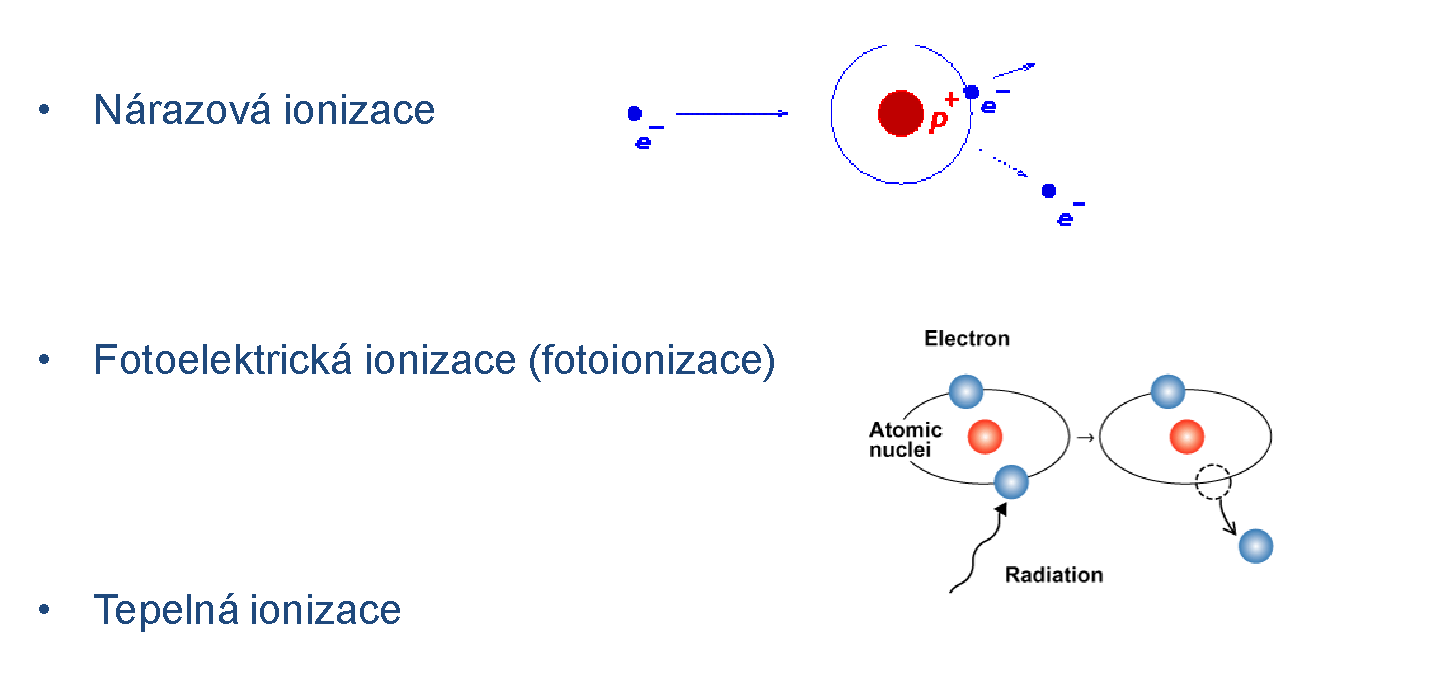
\includegraphics[width=\linewidth,height=52mm,keepaspectratio]{obrazky/emv1_p3_s41.pdf}
\par\vspace{1mm}{\scriptsize\sffamily\color{muted} Nárazový, fotoelektrický a tepelný ionizační mechanismus. P3, s. 41.\par}
\end{minipage}
\par\end{minipage}\par\vspace{6mm}
\noindent\begin{minipage}[b]{\linewidth}
\section*{21. Nakreslete VA-charakteristiku plynové výbojky a detailně popište všechny 4 oblasti.}
Při pevné vzdálenosti elektrod $d$ a ploše $S$ odpovídá zobrazený graf $J(E)$ VA-charakteristice $I(U)$: $E=U/d$, $I=JS$.
\begin{enumerate}
\item \textbf{Ohmická oblast:} slabé pole, převážná část iontů rekombinuje v plynu a jen malá část dojde k elektrodám. Koncentrace nosičů je přibližně stálá, proud roste úměrně napětí.
\item \textbf{Přechodová oblast:} s rostoucím polem více nosičů dosáhne elektrod, rekombinace ubývá. Proud již neroste přímo úměrně napětí a blíží se nasycení.
\item \textbf{Nasycení:} prakticky všechny nosiče vytvořené vnějším ionizátorem dojdou k elektrodám. Proud je určen rychlostí jejich vzniku a na napětí téměř nezávisí.
\item \textbf{Nárazová ionizace:} elektrony získají energii k ionizaci dalších molekul, vznikají elektronové laviny a proud prudce roste. Po splnění Townsendovy podmínky se výboj stane samostatným.
\end{enumerate}
Oblasti I--III a počátek IV vyžadují vnější ionizaci.

\par\vspace{2mm}
\begin{minipage}[t]{.94\linewidth}\centering
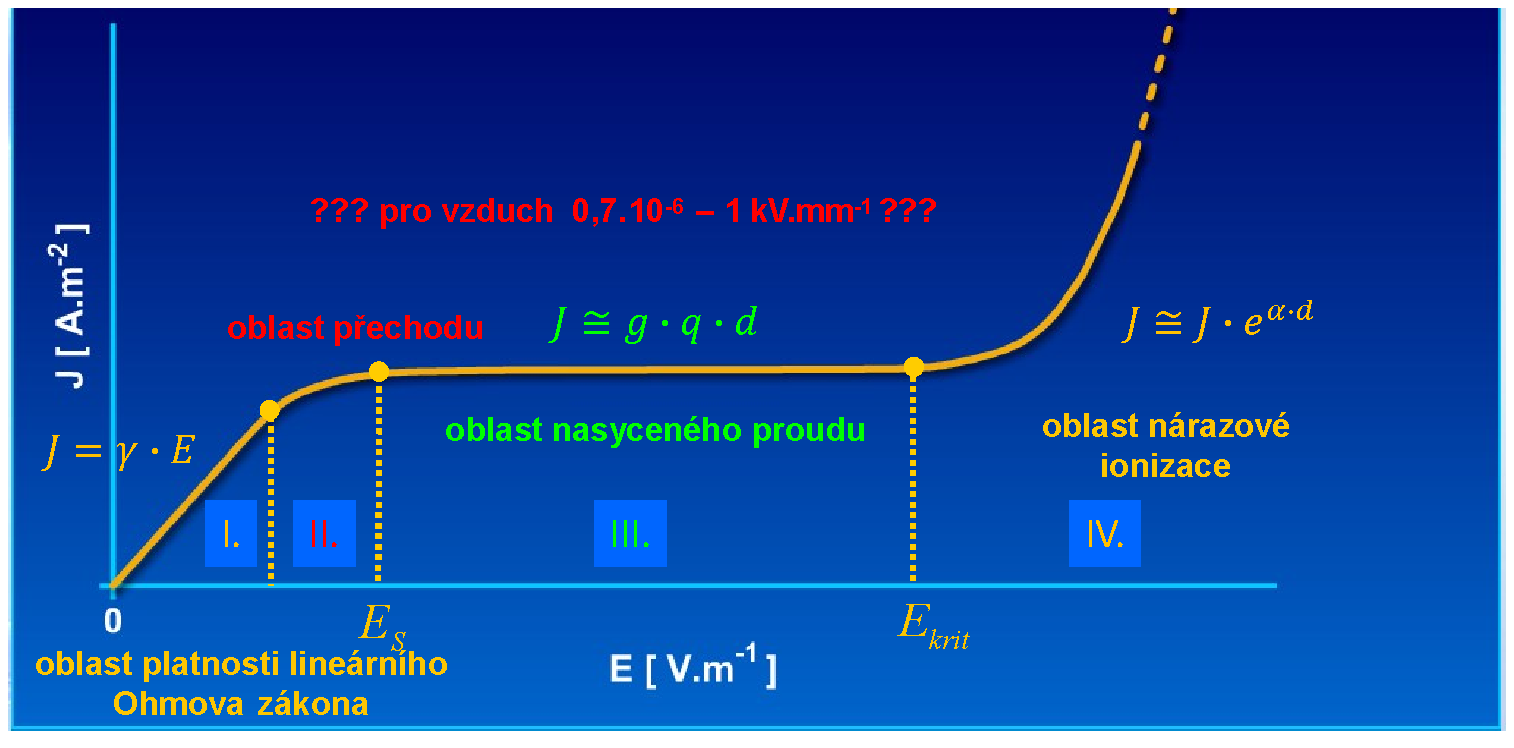
\includegraphics[width=\linewidth,height=52mm,keepaspectratio]{obrazky/emv1_p3_s61.pdf}
\par\vspace{1mm}{\scriptsize\sffamily\color{muted} Čtyři oblasti vodivosti plynu podle přednášky. P3, s. 61.\par}
\end{minipage}
\par\end{minipage}\par\vspace{6mm}
\noindent\begin{minipage}[b]{\linewidth}
\section*{22. Vysvětlete pojem rekombinace a neutralizace a jmenujte jednotlivé typy výbojů.}
\begin{itemize}
\item \textbf{Rekombinace:} spojení opačně nabitých částic v objemu plynu, např. elektronu s kladným iontem; zanikají volné nosiče náboje.
\item \textbf{Neutralizace:} zánik náboje iontu na elektrodě přijetím nebo odevzdáním elektronu.
\end{itemize}
Přednáška rozlišuje \textbf{nesamostatné výboje} (tichý, temný), které potřebují vnější ionizaci, a \textbf{samostatné výboje} (doutnavý, obloukový), které se udržují vlastními ionizačními ději.

\par\vspace{2mm}
\begin{minipage}[t]{.94\linewidth}\centering
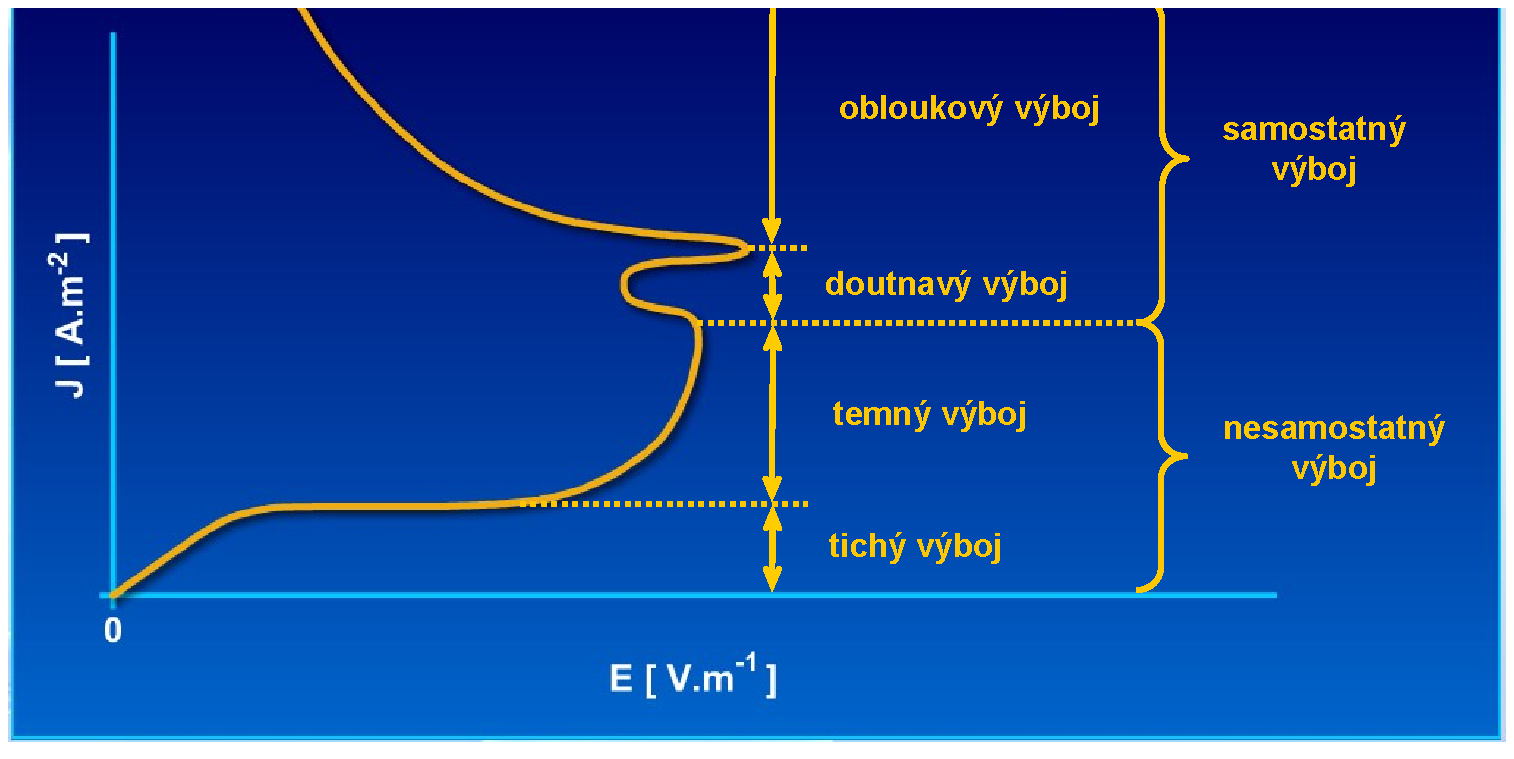
\includegraphics[width=\linewidth,height=52mm,keepaspectratio]{obrazky/emv1_p3_s62.pdf}
\par\vspace{1mm}{\scriptsize\sffamily\color{muted} Nesamostatný, doutnavý a obloukový průběh. P3, s. 62.\par}
\end{minipage}
\par\end{minipage}\par\vspace{6mm}
\noindent\begin{minipage}[b]{\linewidth}
\section*{23. Vysvětlete slovně Townsendovu podmínku samostatného výboje.}
\textbf{Jedna elektronová lavina musí zajistit vznik alespoň jednoho nového elektronu na katodě, který spustí další lavinu.} Kladné ionty vytvořené lavinou dopadají na katodu a uvolňují sekundární elektrony. Tím se proces obnovuje a výboj se udrží i bez vnějšího ionizátoru; na mezi samostatného výboje připadá na původní elektron právě jeden takto vytvořený následník.

\par\vspace{2mm}
\begin{minipage}[t]{.94\linewidth}\centering
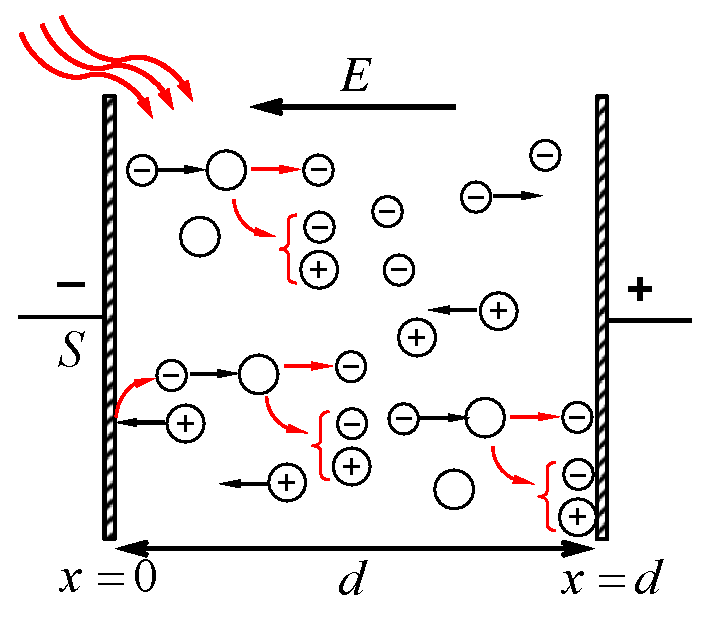
\includegraphics[width=\linewidth,height=52mm,keepaspectratio]{obrazky/emv1_p3_s57.pdf}
\par\vspace{1mm}{\scriptsize\sffamily\color{muted} Zpětná vazba přes kladné ionty a katodu. P3, s. 57.\par}
\end{minipage}
\par\end{minipage}\par\vspace{6mm}
\noindent\begin{minipage}[b]{\linewidth}
\section*{24. Co vyjadřují Townsendovy ionizační součinitelé α, β a γ ?}
\begin{itemize}
\item \textbf{$\alpha$ [m$^{-1}$]:} počet ionizačních dějů vyvolaných jedním elektronem na jednotkové dráze; popisuje růst elektronové laviny.
\item \textbf{$\beta$ [m$^{-1}$]:} počet ionizačních dějů vyvolaných jedním kladným iontem na jednotkové dráze; obvykle mnohem menší příspěvek.
\item \textbf{$\gamma$ [1]:} průměrný počet sekundárních elektronů uvolněných z katody jedním dopadajícím kladným iontem; umožňuje zpětnou vazbu výboje.
\end{itemize}

\par\vspace{2mm}
\begin{minipage}[t]{.94\linewidth}\centering
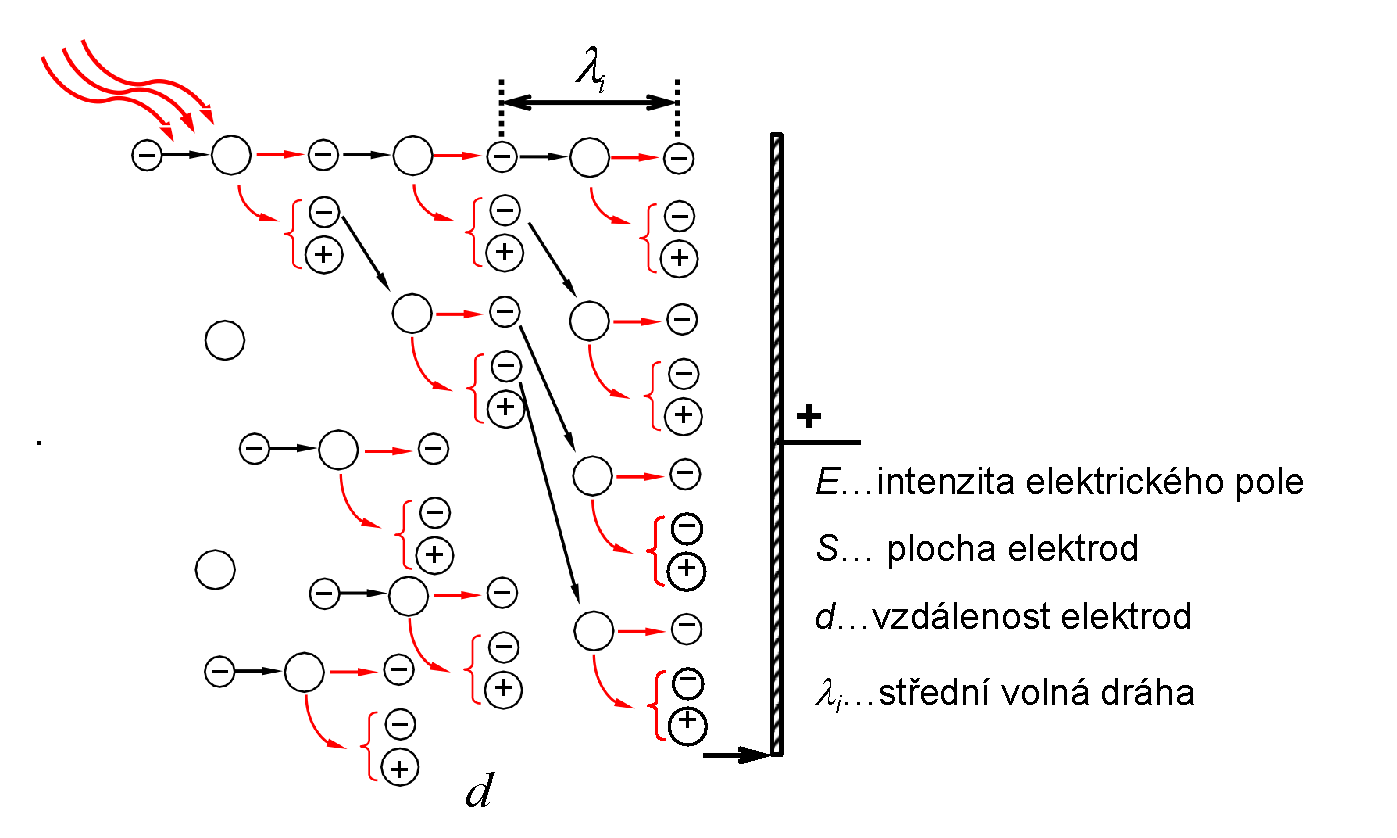
\includegraphics[width=\linewidth,height=52mm,keepaspectratio]{obrazky/emv1_p3_s53.pdf}
\par\vspace{1mm}{\scriptsize\sffamily\color{muted} Násobení elektronů při průchodu plynem. P3, s. 53.\par}
\end{minipage}
\par\end{minipage}\par\vspace{6mm}
\noindent\begin{minipage}[b]{\linewidth}
\section*{25. Vysvětlete Paschenovu křivku, co platí pro body na této křivce a k čemu ji lze využít?}
\textbf{Paschenova křivka} vyjadřuje závislost zápalného napětí na součinu tlaku plynu $p$ a vzdálenosti elektrod $d$:
\[U_z=f(pd).\]
Pro daný plyn a materiál elektrod odpovídá stejnému $pd$ stejné $U_z$. Křivka má minimum; při menším i větším $pd$ zápalné napětí roste.

Všechny její body splňují \textbf{mezní Townsendovu podmínku samostatného výboje} $\gamma(e^{\alpha d}-1)=1$. Křivka odděluje oblast nesamostatného a samostatného výboje.

Slouží k určení zápalného napětí pro daný tlak a mezeru, případně k volbě tlaku či vzdálenosti elektrod pro požadované zápalné napětí.

\par\vspace{2mm}
\begin{minipage}[t]{.94\linewidth}\centering
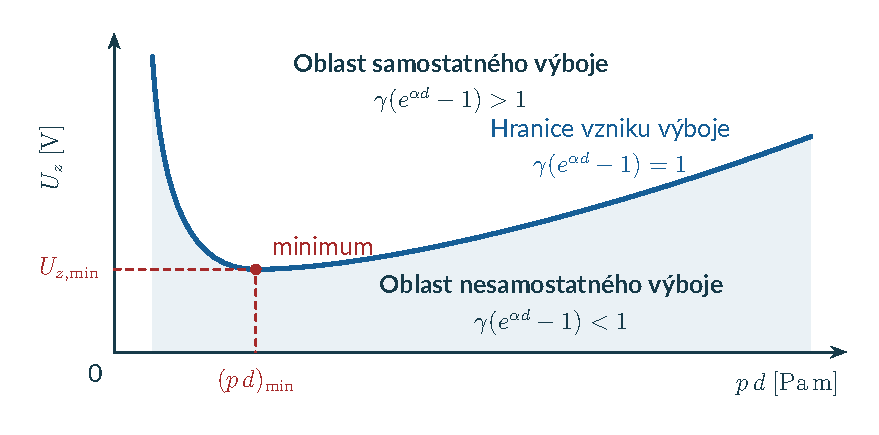
\includegraphics[width=\linewidth,height=52mm,keepaspectratio]{obrazky/emv1_p3_s66.pdf}
\par\vspace{1mm}{\scriptsize\sffamily\color{muted} Paschenova křivka -- schematicky překresleno podle přednášky. P3, s. 66.\par}
\end{minipage}
\par\end{minipage}\par\vspace{6mm}
\noindent\begin{minipage}[b]{\linewidth}
\section*{26. Popište strukturu azbestu a jeho vlastnosti či související rizika a jmenujte možné oblasti použití.}
\textbf{Azbest} je vláknitý krystalický silikát s pásovou strukturou.
\begin{itemize}
\item \textbf{Vlastnosti:} vláknitost, vysoká tepelná odolnost a dobré elektroizolační vlastnosti; rezistivita přibližně $10^8$--$10^{10}\,\Omega\,\mathrm m$.
\item \textbf{Rizika:} jemná vlákna se usazují v plicích, způsobují azbestózu a mají karcinogenní účinky.
\item \textbf{Použití:} z dlouhých vláken tepelně odolné příze a tkaniny, z kratších izolační papír a lepenka, z velmi krátkých azbestocement; tepelné a elektrické izolace.
\end{itemize}

\par\vspace{2mm}
\begin{minipage}[t]{.94\linewidth}\centering
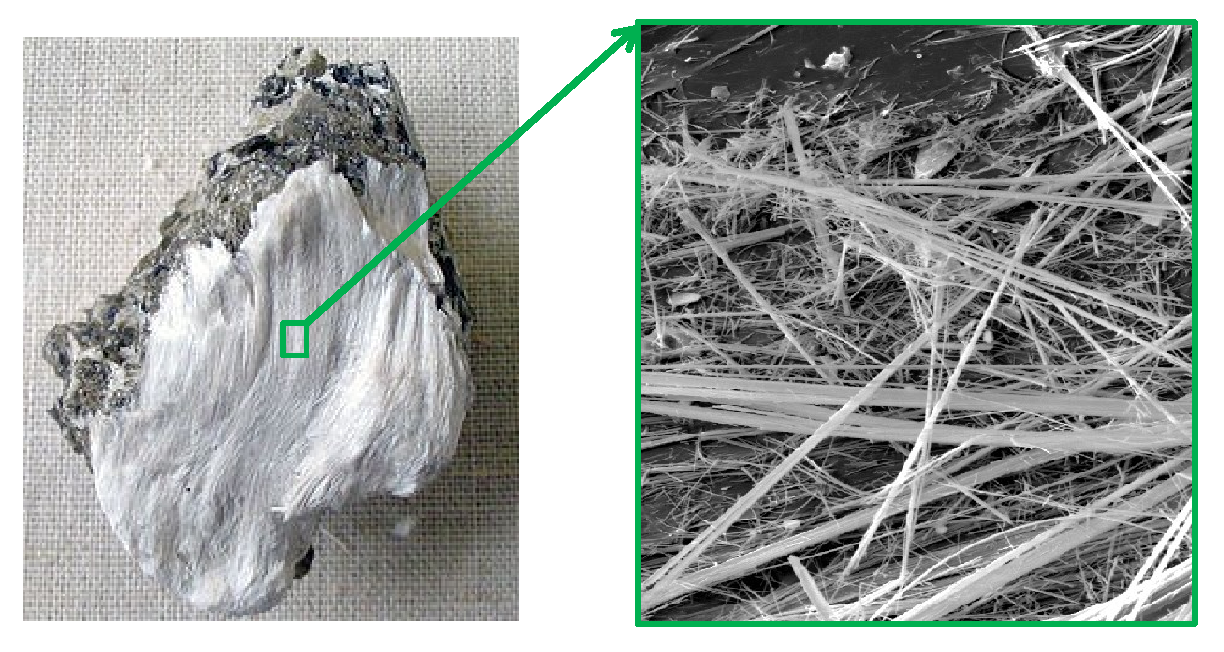
\includegraphics[width=\linewidth,height=52mm,keepaspectratio]{obrazky/emv1_p4_s13.pdf}
\par\vspace{1mm}{\scriptsize\sffamily\color{muted} Vláknitá struktura azbestu. P4, s. 13.\par}
\end{minipage}
\par\end{minipage}\par\vspace{6mm}
\noindent\begin{minipage}[b]{\linewidth}
\section*{27. Popište vnitřní strukturu slídy, vypište její význačné vlastnosti a příklady použití.}
\textbf{Slída} je vrstevnatý silikát s plošnou strukturou. Jednotlivé listy jsou propojeny draselnými ionty; vrstevnatost umožňuje štípání na tenké lístky.
\begin{itemize}
\item \textbf{Vlastnosti:} dokonalá štípatelnost, pružnost a ohebnost lístků, nehořlavost, chemická a tepelná odolnost, vysoká rezistivita a elektrická pevnost, malé dielektrické ztráty.
\item \textbf{Použití:} izolace komutátorů a vinutí strojů, nosiče topných drátů, izolační podložky a slídové kondenzátory.
\end{itemize}

\par\vspace{2mm}
\begin{minipage}[t]{.94\linewidth}\centering
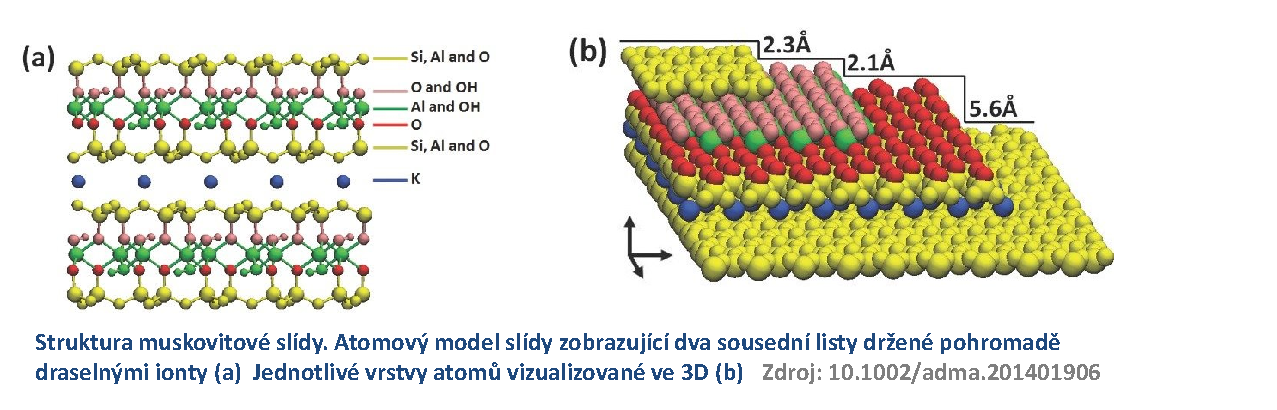
\includegraphics[width=\linewidth,height=52mm,keepaspectratio]{obrazky/emv1_p4_s16.pdf}
\par\vspace{1mm}{\scriptsize\sffamily\color{muted} Vrstvy slídy a jejich propojení draselnými ionty. P4, s. 16.\par}
\end{minipage}
\par\end{minipage}\par\vspace{6mm}
\noindent\begin{minipage}[b]{\linewidth}
\section*{28. Jmenujte obchodní druhy slíd a vysvětlete pojmy mikanit, mikalex a mikafólium.}
\textbf{Obchodní druhy:} slída bloková (tabulková), kalibrovaná, štípaná (splitting), mletá a mikromletá.
\begin{itemize}
\item \textbf{Mikanit:} vrstvený izolační materiál ze slídových lístků nebo slídového papíru spojených pojivem, např. šelakem či pryskyřicí.
\item \textbf{Mikalex:} materiál z mleté slídy (asi 60\,\%) a nízkoztrátového skla (asi 40\,\%), zpracovaný lisováním.
\item \textbf{Mikafólium:} ohebný slídový materiál s pojivem a podložkou, dodávaný ve svitcích pro tvarování izolací.
\end{itemize}

\par\end{minipage}\par\vspace{6mm}
\noindent\begin{minipage}[b]{\linewidth}
\section*{29. Popište skelný stav látek a zakreslete strukturu křemenného a křemičitého skla, v čem se liší jednotlivé formy z pohledu permitivity, ztrát a propustnosti pro různé typy záření.}
\textbf{Skelný stav} je amorfní pevný stav bez pravidelné prostorové mřížky. Sklo je termodynamicky nestabilní a místo ostrého bodu tání postupně měkne.
\begin{itemize}
\item \textbf{Křemenné sklo:} síť tvoří SiO$_2$ bez modifikačních iontů. Má nízkou permitivitu ($\varepsilon_r\approx3{,}8$) a malé ztráty ($\tan\delta\approx2\cdot10^{-4}$); propouští viditelné i UV záření.
\item \textbf{Křemičité sklo:} síť obsahuje další oxidy a modifikační ionty. Permitivita i ztráty závisejí na složení; pohyblivé ionty zvyšují ztráty. Nízkoztrátová olovnatá skla mají $\varepsilon_r\approx7$--$8$, boritokřemičitá $4$--$5$. Křemičitá skla propouštějí především viditelné záření.
\end{itemize}
Pro \textbf{infračervené záření} se používají např. bezkyslíkatá chalkogenidová skla As--S.

\par\vspace{2mm}
\begin{minipage}[t]{.94\linewidth}\centering
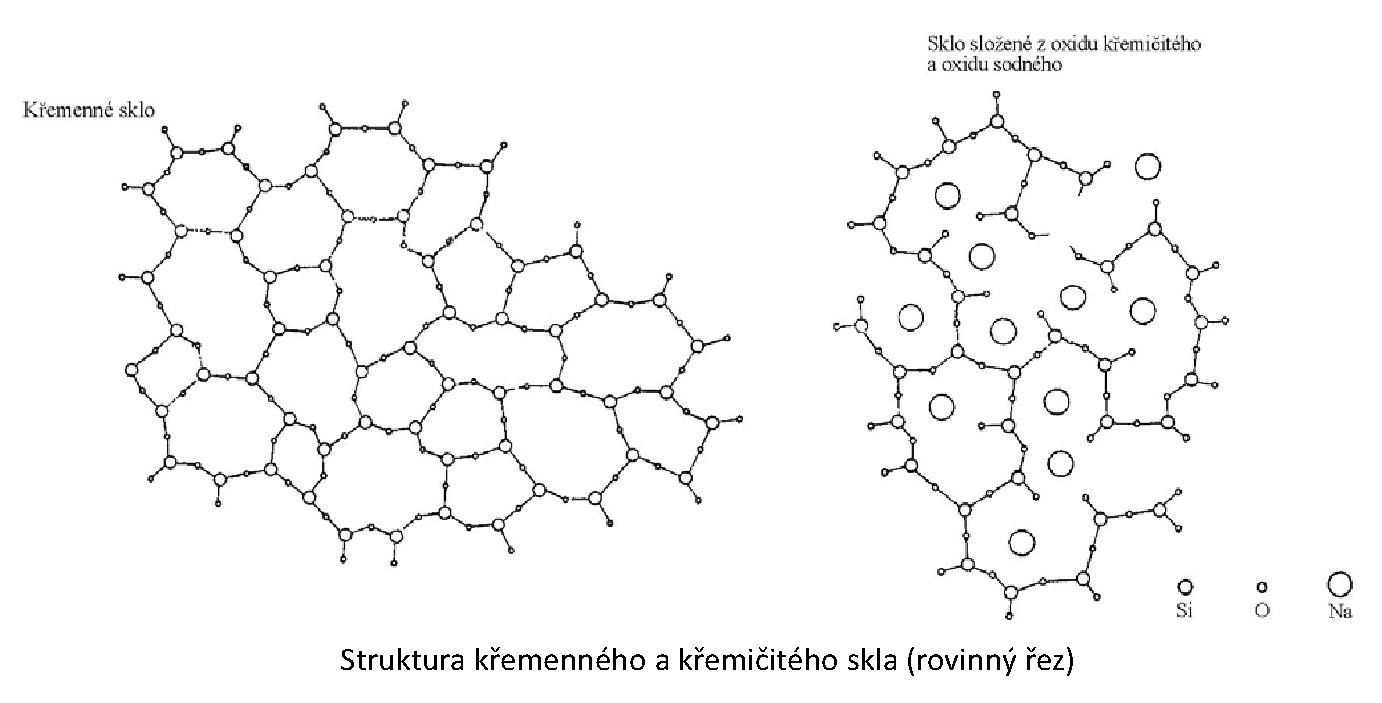
\includegraphics[width=\linewidth,height=52mm,keepaspectratio]{obrazky/emv1_p4_s29.pdf}
\par\vspace{1mm}{\scriptsize\sffamily\color{muted} Křemenná síť a síť modifikovaná ionty. P4, s. 29.\par}
\end{minipage}
\par\end{minipage}\par\vspace{6mm}
\noindent\begin{minipage}[b]{\linewidth}
\section*{30. Jmenujte různé skupiny látek přidávaných do sklářského kmene a vysvětlete jejich funkci.}
Do sklářského kmene se přidávají:
\begin{itemize}
\item \textbf{Urychlovače tavení:} urychlují tavení či čeření; borax, kyselina boritá, fluoridy, křemičitan sodný.
\item \textbf{Čeřiva:} uvolňují plyny, které odnášejí bubliny ze skloviny; Na$_2$SO$_4$ nebo směs As$_2$O$_3$ a KNO$_3$.
\item \textbf{Barviva:} způsobují zbarvení rozpuštěnými ionty či molekulami nebo koloidními částicemi.
\item \textbf{Odbarviva:} zajišťují čirost a průzračnost; arsenik, ledek, MnO$_2$.
\item \textbf{Kaliva:} částice s odlišným indexem lomu způsobují zákal; např. kryolit Na$_3$AlF$_6$.
\end{itemize}

\par\end{minipage}\par\vspace{6mm}
\noindent\begin{minipage}[b]{\linewidth}
\section*{31. Jaké způsoby čeření skloviny znáte? Popište.}
\textbf{Čeření} odstraňuje drobné plynové bubliny ze skloviny. Přednáška rozlišuje:
\begin{itemize}
\item \textbf{Chemické čeření:} čeřiva, např. Na$_2$SO$_4$ či směs As$_2$O$_3$ a KNO$_3$, za vysoké teploty uvolňují plyny. Ty postupují k povrchu a strhávají s sebou bubliny z objemu skloviny.
\item \textbf{Fyzikální čeření:} únik bublin se usnadní snížením viskozity skloviny při vyšší teplotě; ve viskózní sklovině jinak bubliny stoupají pomalu.
\end{itemize}
Oba způsoby lze kombinovat.

\par\vspace{2mm}
\begin{minipage}[t]{.94\linewidth}\centering
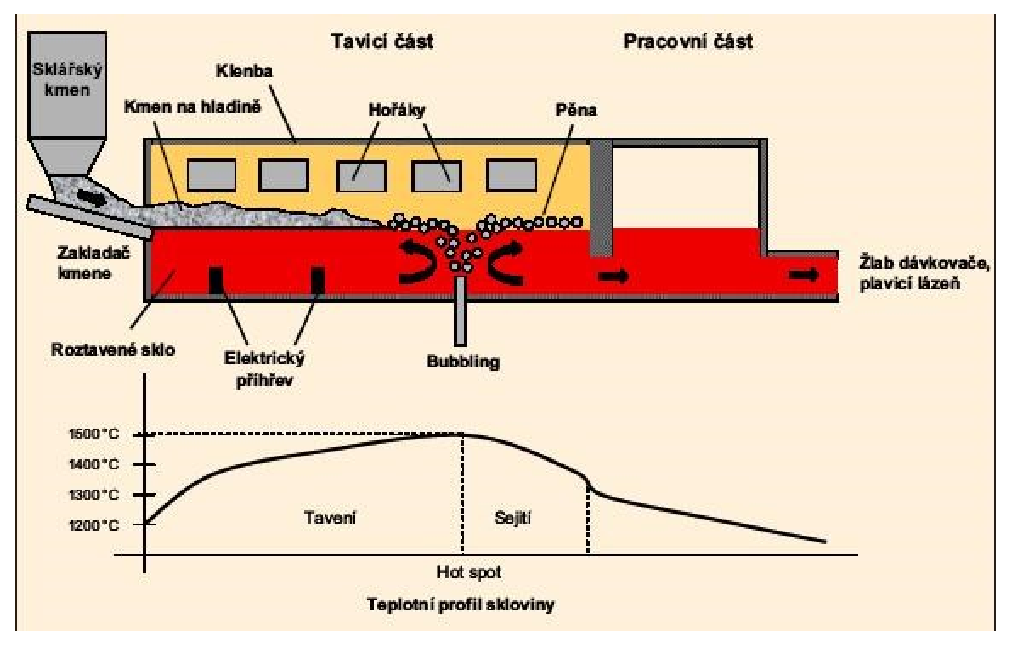
\includegraphics[width=\linewidth,height=52mm,keepaspectratio]{obrazky/emv1_p4_s38.pdf}
\par\vspace{1mm}{\scriptsize\sffamily\color{muted} Tavicí a čeřicí část vanové pece. P4, s. 38.\par}
\end{minipage}
\par\end{minipage}\par\vspace{6mm}
\noindent\begin{minipage}[b]{\linewidth}
\section*{32. Načrtněte závislost logaritmu viskozity na teplotě a jmenujte a popište alespoň čtyři technologicky důležité body.}
Dekadický logaritmus viskozity s rostoucí teplotou nelineárně klesá. Pro $\eta$ v Pa\,s jsou důležité body:
\begin{itemize}
\item \textbf{Dolní chladicí teplota:} $\log\eta=13{,}5$; dolní hranice transformačního intervalu.
\item \textbf{Transformační teplota $T_g$:} $\log\eta=12{,}3$; přechod mezi skelným a podchlazeným kapalným stavem.
\item \textbf{Horní chladicí teplota $T_a$:} $\log\eta=12$; za 15 minut se vnitřní pnutí sníží na přibližně 10\,\%.
\item \textbf{Dolní a horní teplota tvarování:} $\log\eta=7$ a $3$; vymezují pracovní oblast tvarování skla.
\item \textbf{Teplota tavení:} $\log\eta\approx1$; sklovina má nízkou viskozitu vhodnou pro tavení a čeření.
\end{itemize}

\par\vspace{2mm}
\begin{minipage}[t]{.94\linewidth}\centering
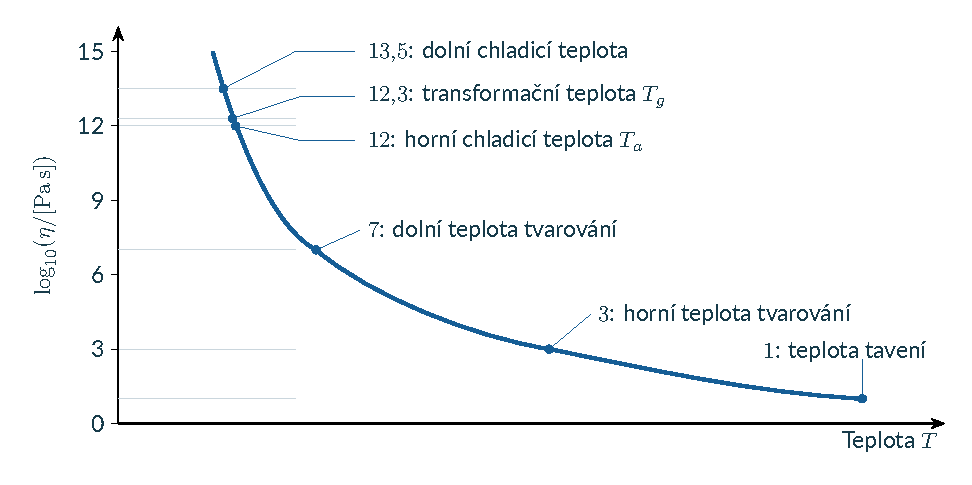
\includegraphics[width=\linewidth,height=52mm,keepaspectratio]{obrazky/emv1_p4_s41.pdf}
\par\vspace{1mm}{\scriptsize\sffamily\color{muted} Viskozitní křivka; schematicky podle s. 40--41, názvy bodů podle s. 40. P4, s. 41.\par}
\end{minipage}
\par\end{minipage}\par\vspace{6mm}
\noindent\begin{minipage}[b]{\linewidth}
\section*{33. Popište proces výroby skleněných vláken pro optiku a konstrukčních vláken.}
\begin{itemize}
\item \textbf{Optická vlákna:} konec preformy se zahřeje v peci a vytahuje na vlákno. Měří se průměr a zpětnou vazbou řídí tažení. Nanese se primární ochranný povlak, vytvrdí se, zkontroluje se jeho tloušťka a vlákno se navine.
\item \textbf{Konstrukční vlákna:} bezalkalické sklo se taví v nádobě s Pt--Rh tryskami; doplňování skleněných kuliček udržuje hladinu taveniny. Vlákna se protahují tryskami, opatří lubrikací a ochranným polymerním povlakem a navíjejí.
\end{itemize}

\par\vspace{2mm}
\begin{minipage}[t]{.48\linewidth}\centering
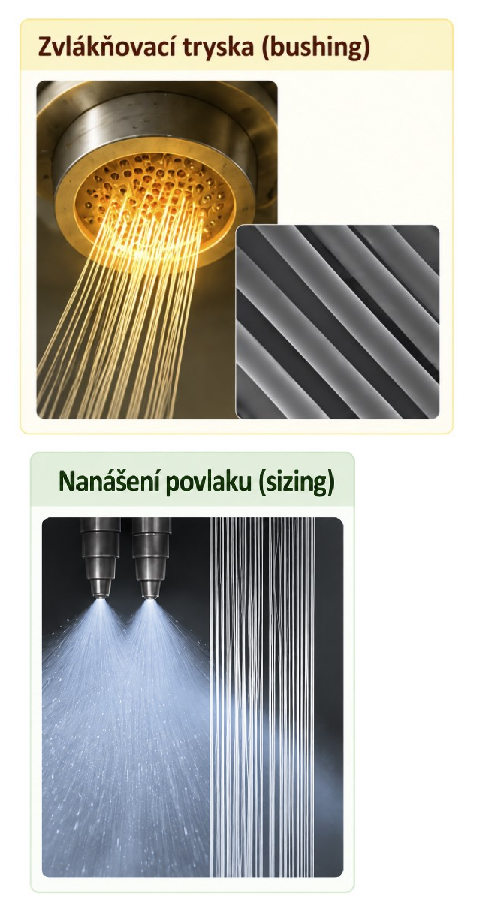
\includegraphics[width=\linewidth,height=52mm,keepaspectratio]{obrazky/emv1_p4_s52.pdf}
\par\vspace{1mm}{\scriptsize\sffamily\color{muted} Zvlákňovací tryska a nanášení apretury. P4, s. 52.\par}
\end{minipage}\hfill
\begin{minipage}[t]{.48\linewidth}\centering
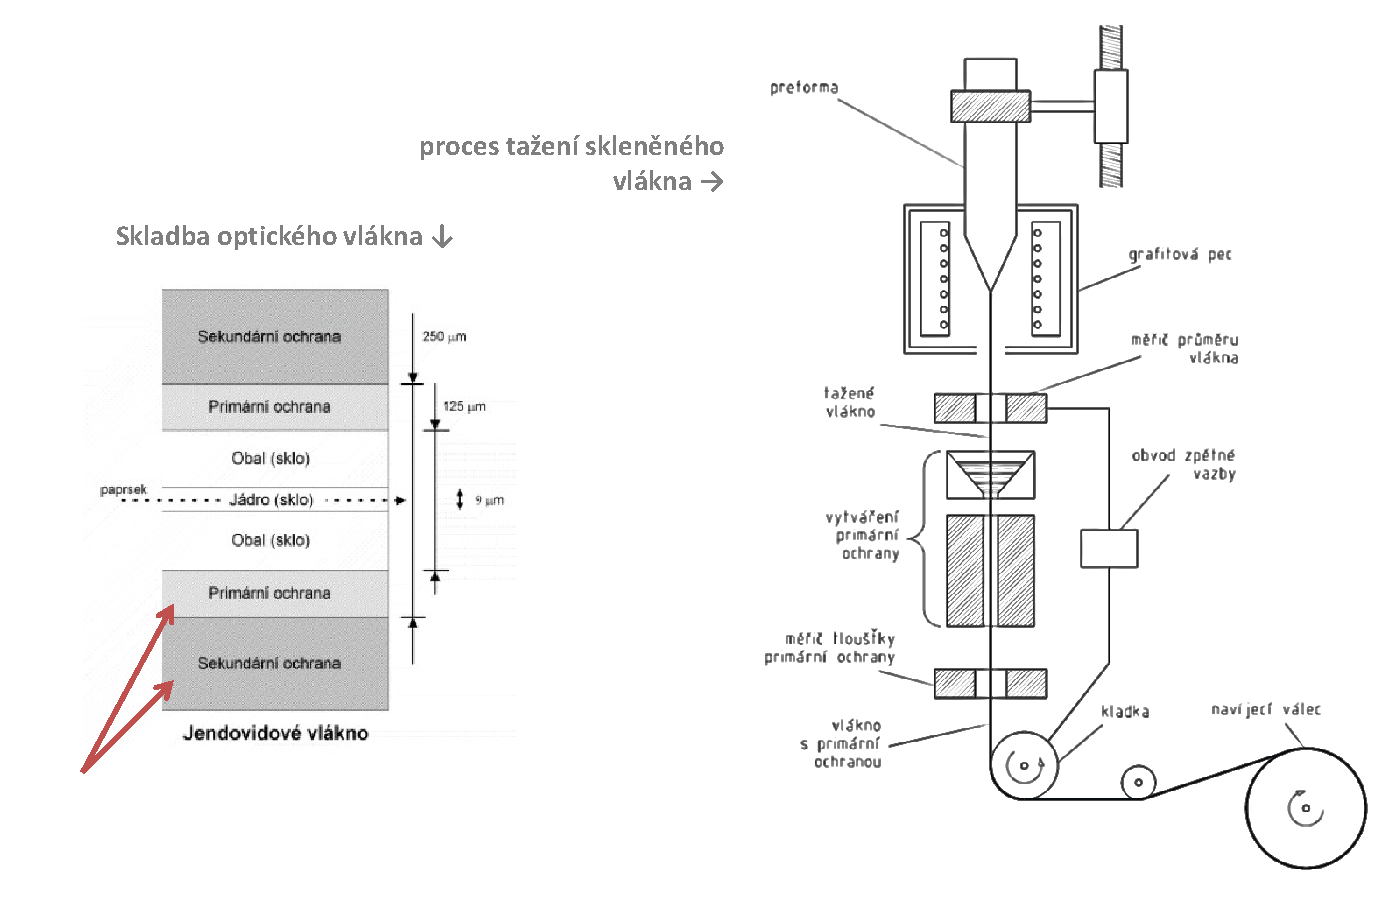
\includegraphics[width=\linewidth,height=52mm,keepaspectratio]{obrazky/emv1_p4_s53.pdf}
\par\vspace{1mm}{\scriptsize\sffamily\color{muted} Tažení optického vlákna a jeho ochranné vrstvy. P4, s. 53.\par}
\end{minipage}
\par\end{minipage}\par\vspace{6mm}
\noindent\begin{minipage}[b]{\linewidth}
\section*{34. Co jsou to skelně krystalické látky a vysvětlete pojmy krystalizace a nukleace.}
\textbf{Skelně krystalické látky (sklokeramiky)} obsahují jemné krystaly ve zbytkové skelné fázi. Vznikají řízeným tepelným zpracováním předem vytvarovaného skla.
\begin{itemize}
\item \textbf{Nukleace:} vznik stabilních krystalizačních zárodků, podporovaný např. nukleátory TiO$_2$ či ZrO$_2$.
\item \textbf{Krystalizace:} vznik a následný růst uspořádané krystalické fáze z původního skla.
\end{itemize}

\par\vspace{2mm}
\begin{minipage}[t]{.94\linewidth}\centering
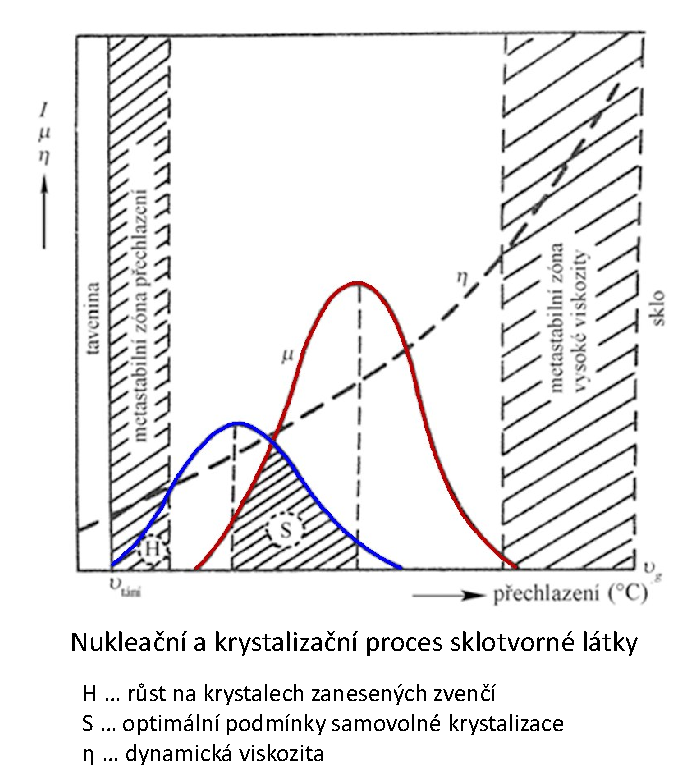
\includegraphics[width=\linewidth,height=52mm,keepaspectratio]{obrazky/emv1_p4_s31.pdf}
\par\vspace{1mm}{\scriptsize\sffamily\color{muted} Teplotní oblasti nukleace a růstu krystalů. P4, s. 31.\par}
\end{minipage}
\par\end{minipage}\par\vspace{6mm}
\noindent\begin{minipage}[b]{\linewidth}
\section*{35. Popište skelný stav a keramický sloh, čím se od sebe liší?}
\begin{itemize}
\item \textbf{Skelný stav:} amorfní uspořádání bez pravidelné prostorové mřížky, vzniklé ztuhnutím taveniny bez krystalizace. Sklo je izotropní, termodynamicky nestabilní a měkne v teplotním intervalu.
\item \textbf{Keramický sloh:} směs \textbf{krystalických zrn, amorfní skelné fáze a plynné fáze v pórech}, vznikající při výpalu keramiky.
\end{itemize}
Rozdíl spočívá v uspořádání: skelný stav je amorfní, keramický sloh kombinuje více fází.

\par\end{minipage}\par\vspace{6mm}
\noindent\begin{minipage}[b]{\linewidth}
\section*{36. V čem jsou význačné materiály jako - steatit, forsterit, kordierit či pyrostat}
\begin{itemize}
\item \textbf{Steatit:} hořečnatá keramika z mastku; malé dielektrické ztráty a dobrá izolace, vhodná pro vf izolátory a podpěry.
\item \textbf{Forsterit (Mg$_2$SiO$_4$):} dobré izolační vlastnosti i za zvýšené teploty; tepelně namáhané izolace.
\item \textbf{Kordierit:} hořečnato-hlinitý silikát s velmi malou teplotní roztažností; odolnost proti tepelným šokům, nosiče topných drátů.
\item \textbf{Pyrostat:} pórovitá hořečnatá keramika s malou tepelnou vodivostí; tepelná izolace a nosná tělesa v topné technice.
\end{itemize}

\par\vspace{2mm}
\begin{minipage}[t]{.94\linewidth}\centering
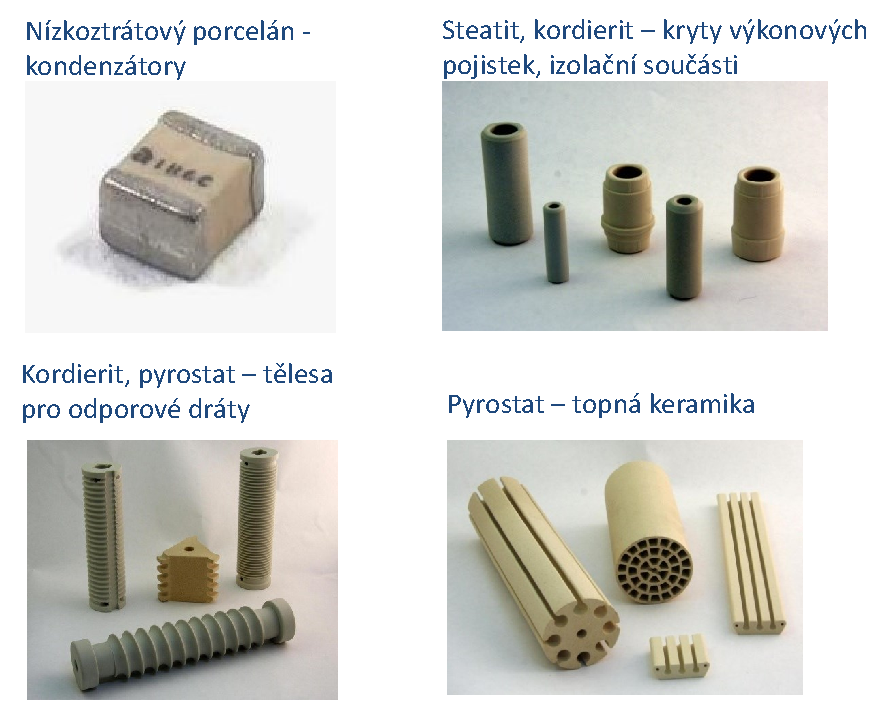
\includegraphics[width=\linewidth,height=52mm,keepaspectratio]{obrazky/emv1_p4_s59.pdf}
\par\vspace{1mm}{\scriptsize\sffamily\color{muted} Příklady výrobků ze speciálních silikátových keramik. P4, s. 59.\par}
\end{minipage}
\par\end{minipage}\par\vspace{6mm}
\noindent\begin{minipage}[b]{\linewidth}
\section*{37. Popište základní kroky při výrobě keramických materiálů.}
\begin{enumerate}
\item \textbf{Úprava surovin:} drcení, mletí, třídění a odstranění nečistot.
\item \textbf{Příprava surové keramické hmoty:} dávkování, míchání, homogenizace a úprava obsahu vody.
\item \textbf{Tváření:} lití, vytlačování, točení nebo lisování.
\item \textbf{Sušení:} odstranění vody z polotovaru.
\item \textbf{Výpal:} chemické a fázové změny, slinování a spojování částic.
\item \textbf{Glazování, je-li požadováno:} vytvoření sklovité povrchové vrstvy.
\item \textbf{Konečná úprava, je-li potřebná:} např. broušení, vrtání či pokovování.
\item \textbf{Technická kontrola} výrobku.
\end{enumerate}

\par\vspace{2mm}
\begin{minipage}[t]{.94\linewidth}\centering
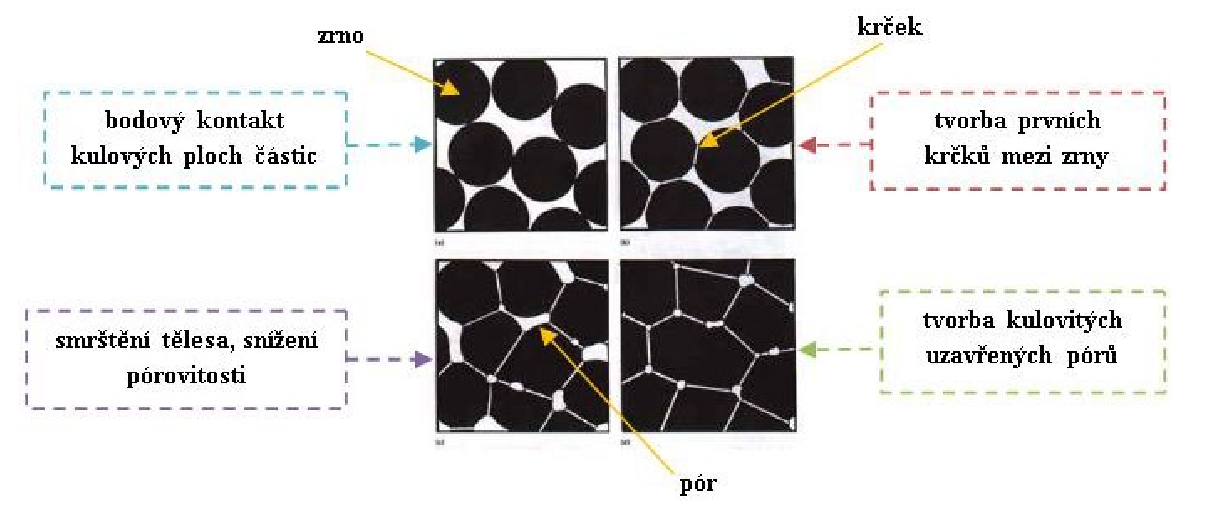
\includegraphics[width=\linewidth,height=52mm,keepaspectratio]{obrazky/emv1_p4_s70.pdf}
\par\vspace{1mm}{\scriptsize\sffamily\color{muted} Vznik krčků, zhutňování a uzavírání pórů při slinování. P4, s. 70.\par}
\end{minipage}
\par\end{minipage}\par\vspace{6mm}
\noindent\begin{minipage}[b]{\linewidth}
\section*{38. Co je to a k čemu slouží glazování keramik.}
\textbf{Glazování} je vytvoření tenké sklovité vrstvy na keramickém střepu. Glazura tvoří hutný a hladký povrch, který brání vnikání vlhkosti, usazování nečistot a vzniku vodivých stop. Zlepšuje elektrické vlastnosti, mechanickou pevnost, odolnost proti povětrnosti a chemickému působení i vzhled výrobku.

\par\end{minipage}\par\vspace{6mm}
\noindent\begin{minipage}[b]{\linewidth}
\section*{39. Popište typy kondenzátorových keramik a vysvětlete jak se liší.}
\begin{itemize}
\item \textbf{Typ I -- stabilit:} nízkoztrátová keramika, např. rutilová, nízkoztrátový porcelán a steatit. Vhodná pro vysokofrekvenční aplikace a teplotní kompenzaci.
\item \textbf{Typ II -- permitit:} vysokodielektrická feroelektrická keramika na bázi BaTiO$_3$, $\varepsilon_r\approx500$--$15\,000$. Umožňuje větší kapacitu; permitivita výrazně závisí na teplotě, frekvenci a napětí.
\item \textbf{Typ III:} bariérové struktury na bázi BaTiO$_3$ a SrTiO$_3$ s tenkou účinnou dielektrickou vrstvou a vysokou objemovou kapacitou; použití v telekomunikační a mikrovlnné technice.
\end{itemize}

\par\vspace{2mm}
\begin{minipage}[t]{.94\linewidth}\centering
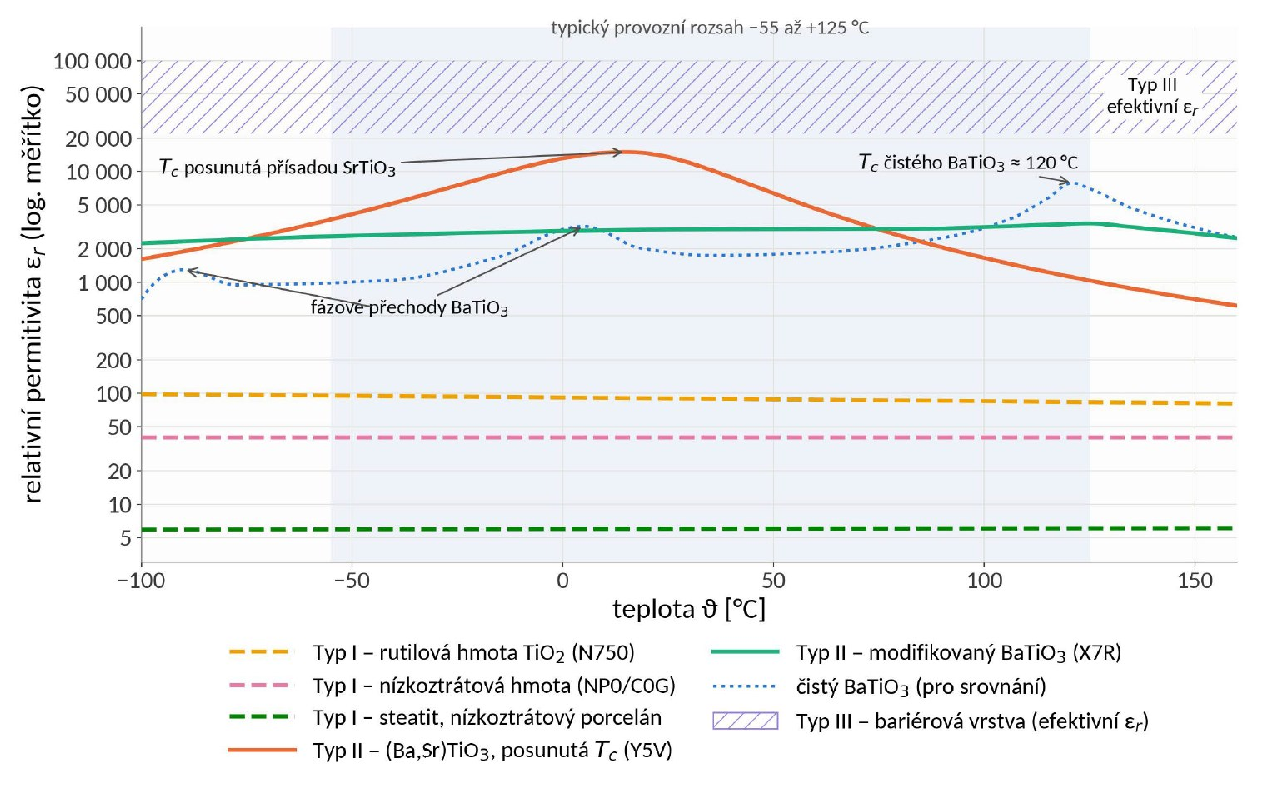
\includegraphics[width=\linewidth,height=52mm,keepaspectratio]{obrazky/emv1_p4_s79.pdf}
\par\vspace{1mm}{\scriptsize\sffamily\color{muted} Teplotní závislosti kapacit keramických hmot. P4, s. 79.\par}
\end{minipage}
\par\end{minipage}\par\vspace{6mm}
\noindent\begin{minipage}[b]{\linewidth}
\section*{40. Nakreslete a popište hysterezní smyčku feroelektrika a vysvětlete pojem Curieova teplota Tc}
Hysterezní smyčka $P(E)$ ukazuje, že polarizace závisí i na předchozím elektrickém poli:
\begin{itemize}
\item Rostoucí pole přepólovává domény až k nasycení.
\item Při návratu na $E=0$ zůstává \textbf{remanentní polarizace $P_r$}.
\item Opačné \textbf{koercitivní pole $-E_c$} sníží polarizaci na nulu; další zesílení pole vede k zápornému nasycení.
\item Zpětná větev prochází zápornou remanencí $-P_r$ a kladným koercitivním polem $+E_c$, čímž se smyčka uzavře.
\end{itemize}
\textbf{Curieova teplota $T_C$} je teplota přechodu z feroelektrického do paraelektrického stavu: zaniká spontánní polarizace. U BaTiO$_3$ je přibližně $120\,^{\circ}\mathrm C$ a v jejím okolí dosahuje permitivita maxima.

\par\vspace{2mm}
\begin{minipage}[t]{.94\linewidth}\centering
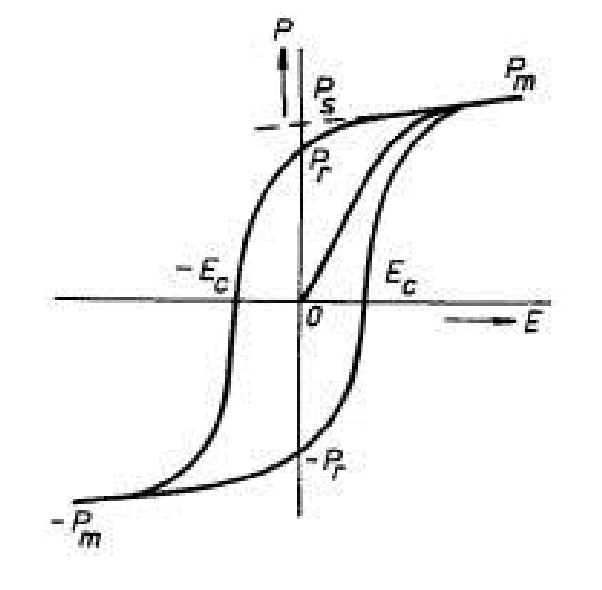
\includegraphics[width=\linewidth,height=52mm,keepaspectratio]{obrazky/emv1_p4_s77.pdf}
\par\vspace{1mm}{\scriptsize\sffamily\color{muted} Feroelektrická hysterezní smyčka P(E). P4, s. 77.\par}
\end{minipage}
\par\end{minipage}\par\vspace{6mm}
\noindent\begin{minipage}[b]{\linewidth}
\section*{41. Vysvětlete pojem pohyblivost, co udává a na čem závisí?}
\textbf{Pohyblivost} udává střední driftovou rychlost nosiče připadající na jednotku intenzity elektrického pole:
\[\boxed{\mu=\frac{|v_d|}{|E|}}\quad[\mathrm{m^2/(V\,s)}].\]
V kovu ji ovlivňuje rozptyl elektronů na tepelných kmitech mřížky, nečistotách, poruchách a hranicích zrn; větší rozptyl pohyblivost snižuje. Závisí tedy na teplotě, čistotě a struktuře materiálu. V kapalinách pohyblivost iontů klesá s viskozitou, přibližně $\mu\sim1/\eta$.

\par\end{minipage}\par\vspace{6mm}
\noindent\begin{minipage}[b]{\linewidth}
\section*{42. Popište vliv nečistot na rezistivitu kovu při nízkých teplotách.}
Nečistoty a poruchy mřížky rozptylují elektrony, snižují pohyblivost a vytvářejí \textbf{zbytkovou rezistivitu $\rho_0$}:
\[\rho(T)\approx\rho_0+\rho_{\mathrm{fonony}}(T).\]
Při nízké teplotě slábne rozptyl na tepelných kmitech, takže převládne $\rho_0$. Čím více nečistot, tím vyšší nenulové plató rezistivity při $T\to0$; čistší kov má nižší $\rho_0$.

\par\vspace{2mm}
\begin{minipage}[t]{.94\linewidth}\centering
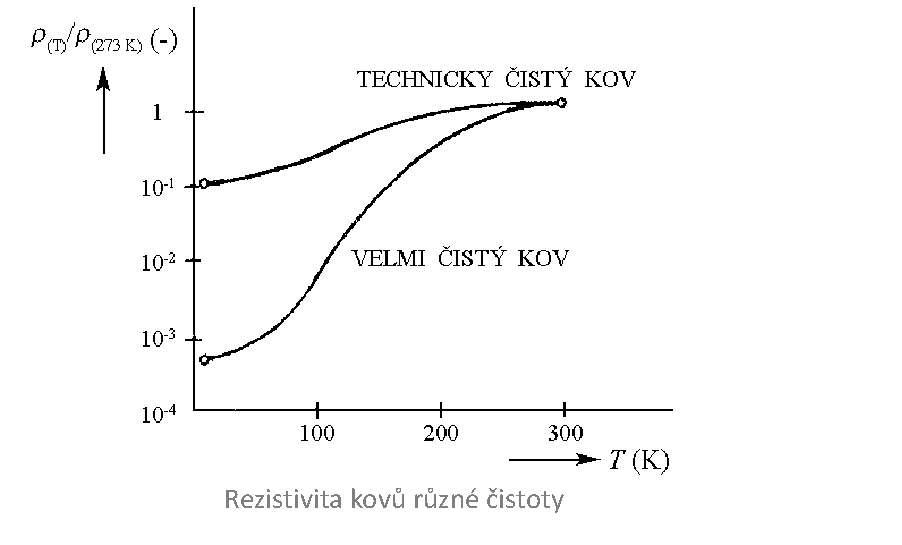
\includegraphics[width=\linewidth,height=52mm,keepaspectratio]{obrazky/emv1_p5_s11.pdf}
\par\vspace{1mm}{\scriptsize\sffamily\color{muted} Vliv čistoty kovu na zbytkovou rezistivitu. P5, s. 11.\par}
\end{minipage}
\par\end{minipage}\par\vspace{6mm}
\noindent\begin{minipage}[b]{\linewidth}
\section*{43. Vyjmenujte různé aplikace použití kovů v elektrotechnice a pro tři aplikační oblasti vyjmenujte požadavky na tyto materiály.}
\textbf{Aplikace kovů:} vodiče a vinutí, odporové prvky, pájky, kontakty, termočlánky, pojistky, vakuová technika a dvojkovy. Požadavky pro tři oblasti:
\begin{itemize}
\item \textbf{Vodiče:} malá rezistivita, dobrá zpracovatelnost a mechanické vlastnosti, odolnost proti korozi, snadné spojování, dostupnost a nízká cena.
\item \textbf{Přesné rezistory:} vhodná rezistivita, malý teplotní součinitel, stabilita odporu a malé termoelektrické napětí vůči mědi.
\item \textbf{Kontakty:} dobrá elektrická a tepelná vodivost, malý stálý přechodový odpor, odolnost proti oxidaci a elektrické erozi, velká tvrdost.
\end{itemize}

\par\end{minipage}\par\vspace{6mm}
\noindent\begin{minipage}[b]{\linewidth}
\section*{44. Stručně popište 4 vybrané jevy spojené s průchodem kovů ve vodičích a představte oblasti ve kterých dochází k jejich uplatnění}
\begin{enumerate}
\item \textbf{Jouleovo teplo:} proud ohřívá odporový vodič, elektrická energie se mění na teplo; význam ve výkonové elektronice, čipech a při odvádění tepla.
\item \textbf{Skin efekt:} střídavý proud se soustřeďuje k povrchu vodiče, čímž roste odpor; důležitý pro vysokofrekvenční spoje a rychlé přenosy.
\item \textbf{Proximity efekt:} pole blízkých vodičů způsobuje nerovnoměrné rozložení proudu a vyšší ztráty; uplatňuje se ve vinutích a transformátorech.
\item \textbf{Hallův jev:} při průchodu proudu v magnetickém poli vzniká příčné napětí kolmé k proudu i poli; Hallovy senzory a měření magnetického pole.
\end{enumerate}

\par\end{minipage}\par\vspace{6mm}
\noindent\begin{minipage}[b]{\linewidth}
\section*{45. Vyjmenujte základní materiály a typy slitin pro pájky a vyjmenujte složky tavidla podporujícího pájecí proces.}
\textbf{Pájky} se podle teploty tavení dělí na měkké a tvrdé. U měkkých pájek přednáška uvádí:
\begin{itemize}
\item \textbf{Olovnaté:} slitiny Sn--Pb, např. SnPb 63/37.
\item \textbf{Bezolovnaté:} Sn s přídavky Ag, Cu, Zn, Bi či Sb, případně Ge; uváděné pájky SAC305 a SN100C.
\end{itemize}
\textbf{Složky tavidla:} nosič (přírodní nebo syntetická pryskyřice, případně báze organických kyselin), aktivátory (organické kyseliny, aminy, halogenidové složky), aditiva a rozpouštědla (např. izopropanol, voda či kombinace).

\par\end{minipage}\par\vspace{6mm}
\noindent\begin{minipage}[b]{\linewidth}
\section*{46. Jmenujte zástupce odporových materiálů pro přesné rezistory a pro odporová tělesa určená pro ohřev.}
\begin{itemize}
\item \textbf{Přesné rezistory:} manganin (Cu--Mn--Ni), konstantan (Cu--Ni s příměsí Mn), slitiny Au--Cr.
\item \textbf{Odporová topná tělesa:} chromnikl/nichrom (Ni--Cr), slitiny Cr--Ni--Fe, kanthal a fechral (Fe--Cr--Al); pro vysoké teploty také Mo a W v inertní atmosféře, SiC a grafit.
\end{itemize}

\par\end{minipage}\par\vspace{6mm}
\noindent\begin{minipage}[b]{\linewidth}
\section*{47. Popište supravodivý stav pomocí BCS teorie, pro které supravodiče platí a jaké faktory mohou způsobit zánik supravodivosti?}
\textbf{BCS teorie:} při nízké teplotě se elektrony s opačnými spiny párují do \textbf{Cooperových párů}. Přitažlivá interakce umožní párování navzdory elektrostatickému odpuzování. Páry vytvářejí společný kvantový koherentní stav, \textbf{BCS kondenzát}, spojený se supravodivostí a nulovou rezistivitou.

Přednáška BCS vysvětluje v souvislosti se \textbf{supravodiči I. třídy}.

Supravodivost zaniká při dosažení \textbf{kritické teploty $T_k$} nebo \textbf{kritické intenzity magnetického pole $H_k$}: Cooperovy páry se rozpadají. Hodnota kritického pole závisí na teplotě, struktuře, čistotě a vnitřním pnutí materiálu.

\par\vspace{2mm}
\begin{minipage}[t]{.94\linewidth}\centering
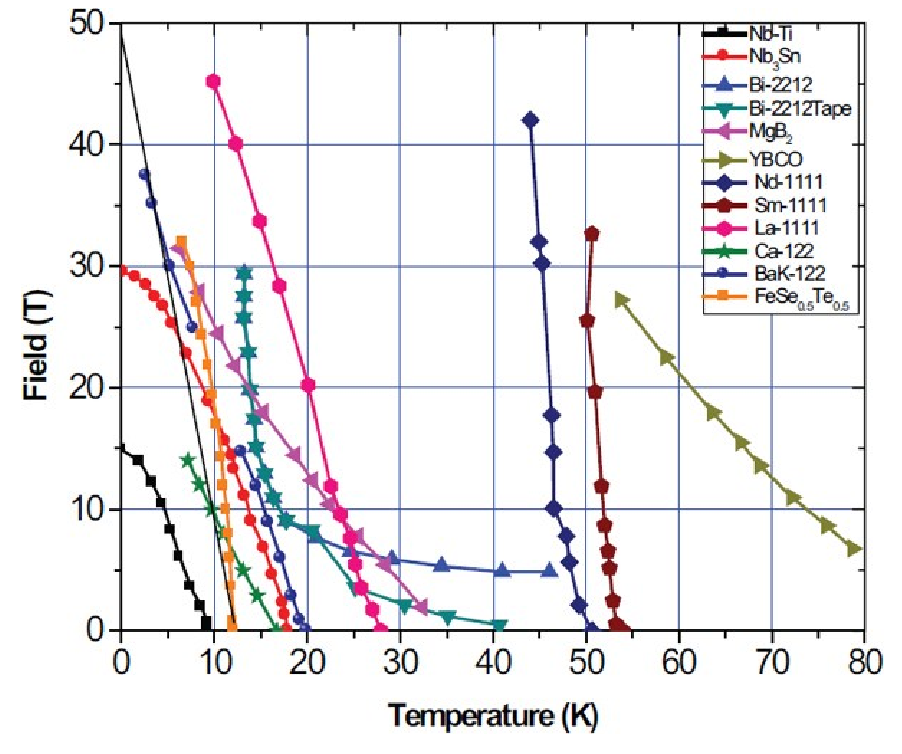
\includegraphics[width=\linewidth,height=52mm,keepaspectratio]{obrazky/emv1_p5_s22.pdf}
\par\vspace{1mm}{\scriptsize\sffamily\color{muted} Kritická mez magnetického pole a teploty. P5, s. 22.\par}
\end{minipage}
\par\end{minipage}\par\vspace{6mm}
\noindent\begin{minipage}[b]{\linewidth}
\section*{48. Načrtněte průběh rezistivity u supravodivého a u běžného kovu, jmenujte zástupce supravodivých materiálů a jmenujte aplikace ve kterých se využívá supravodivosti.}
\textbf{Průběh $\rho(T)$:} u běžného kovu rezistivita při ochlazování plynule klesá k nenulové zbytkové hodnotě $\rho_0$, dané nečistotami. U supravodiče při kritické teplotě $T_k$ prudce klesá na nulu. Graf odporu $R(T)$ má při neměnné geometrii stejný tvar.
\begin{itemize}
\item \textbf{Zástupci:} čisté kovy Hg, Pb, Nb; slitiny Pb--Bi a Nb--Zr; intermetalické sloučeniny Nb$_3$Sn a Nb$_3$Al.
\item \textbf{Aplikace:} supravodivé kabely a silné elektromagnety, zejména magnetické udržení plazmatu v tokamacích a stelarátorech.
\end{itemize}

\par\vspace{2mm}
\begin{minipage}[t]{.94\linewidth}\centering
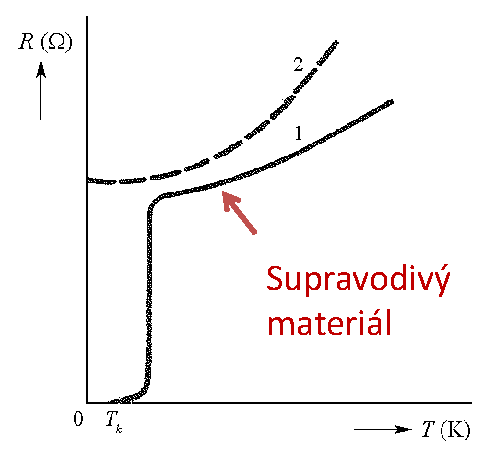
\includegraphics[width=\linewidth,height=52mm,keepaspectratio]{obrazky/emv1_p5_s16.pdf}
\par\vspace{1mm}{\scriptsize\sffamily\color{muted} Odpor při přechodu do supravodivého stavu. P5, s. 16.\par}
\end{minipage}
\par\end{minipage}\par\vspace{6mm}
\noindent\begin{minipage}[b]{\linewidth}
\section*{49. Jaké jsou požadavky na materiály na doteky, jaké materiály se používají a jmenujte konkrétní aplikace.}
\textbf{Požadavky:} dobrá elektrická a tepelná vodivost, malý přechodový odpor, odolnost proti oxidaci a erozi elektrickým proudem, velká tvrdost. Přechodový odpor musí být stálý i při malém proudu, napětí a přítlačné síle.
\begin{itemize}
\item \textbf{Velmi malé proudy a napětí:} Au a slitiny s Pt, Ni či Ag; Pt a Pt--Ir, Re, Pd. Klidové a smykové doteky a spínání malých výkonů ve stejnosměrných, nf a vf obvodech.
\item \textbf{Malá zatížení:} Ag a slitiny s Cu, Pt či Pd, Pt--Ni, mosazi a bronzy. Sdělovací, ovládací a kontrolní přístroje, malé stykače a telefonní ústředny.
\item \textbf{Střední zatížení:} W a slinuté W--Cu, W--Ag, Ag--Ni, Ag--grafit; impulzní doteky.
\end{itemize}

\par\vspace{2mm}
\begin{minipage}[t]{.94\linewidth}\centering
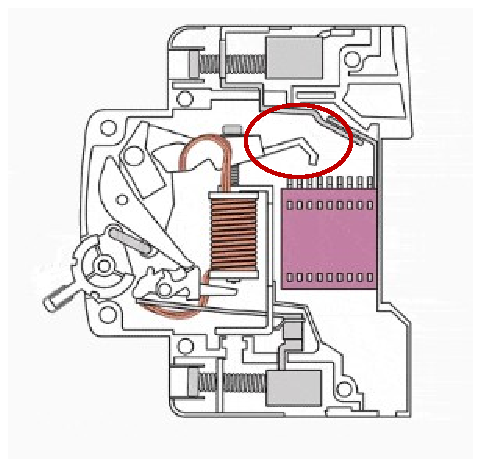
\includegraphics[width=\linewidth,height=52mm,keepaspectratio]{obrazky/emv1_p5_s31.pdf}
\par\vspace{1mm}{\scriptsize\sffamily\color{muted} Kontakt v konstrukci spínacího přístroje. P5, s. 31.\par}
\end{minipage}
\par\end{minipage}\par\vspace{6mm}
\noindent\begin{minipage}[b]{\linewidth}
\section*{50. Popište rozdíly a jmenujte zástupce termoplastů a reaktoplastů.}
\begin{itemize}
\item \textbf{Termoplasty:} lineární nebo rozvětvené řetězce; při ohřevu vratně měknou, lze je opakovaně tvarovat. Zástupci: polyethylen PE, polypropylen PP, polyvinylchlorid PVC, polystyren PS.
\item \textbf{Reaktoplasty:} vytvrzováním vzniká nevratně prostorová síť. Vytvrzený materiál se již netaví ani nerozpouští. Zástupci: fenoplasty, epoxidové pryskyřice a aminoplasty.
\end{itemize}

\par\vspace{2mm}
\begin{minipage}[t]{.94\linewidth}\centering
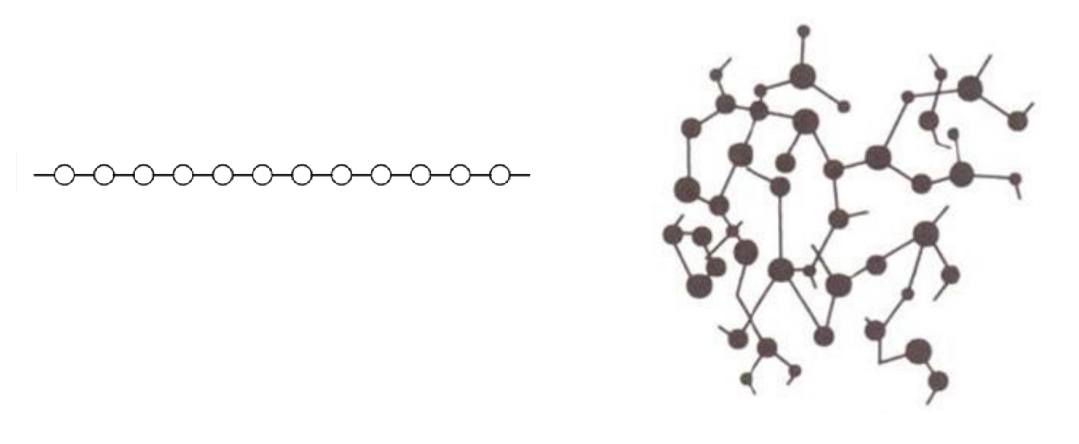
\includegraphics[width=\linewidth,height=52mm,keepaspectratio]{obrazky/emv1_p6_s05.pdf}
\par\vspace{1mm}{\scriptsize\sffamily\color{muted} Lineární řetězec (vlevo) a prostorová síť (vpravo). P6, s. 5.\par}
\end{minipage}
\par\end{minipage}\par\vspace{6mm}
\noindent\begin{minipage}[b]{\linewidth}
\section*{51. Vysvětlete pojmy: stupeň krystalinity, polymerační stupeň makromolekuly, ataktický, syndiotakticky a izotaktický polymer, vulkanizace.}
\begin{itemize}
\item \textbf{Stupeň krystalinity:} podíl krystalické fáze v polymeru.
\item \textbf{Polymerační stupeň:} počet opakujících se základních jednotek v makromolekule.
\item \textbf{Ataktický polymer:} postranní skupiny jsou rozmístěny nepravidelně.
\item \textbf{Syndiotaktický polymer:} postranní skupiny se pravidelně střídají na opačných stranách řetězce.
\item \textbf{Izotaktický polymer:} postranní skupiny mají pravidelně shodné uspořádání na jedné straně řetězce.
\item \textbf{Vulkanizace:} příčné chemické propojení řetězců kaučuku, např. sirnými můstky; vzniká pružná pryž.
\end{itemize}

\par\vspace{2mm}
\begin{minipage}[t]{.94\linewidth}\centering
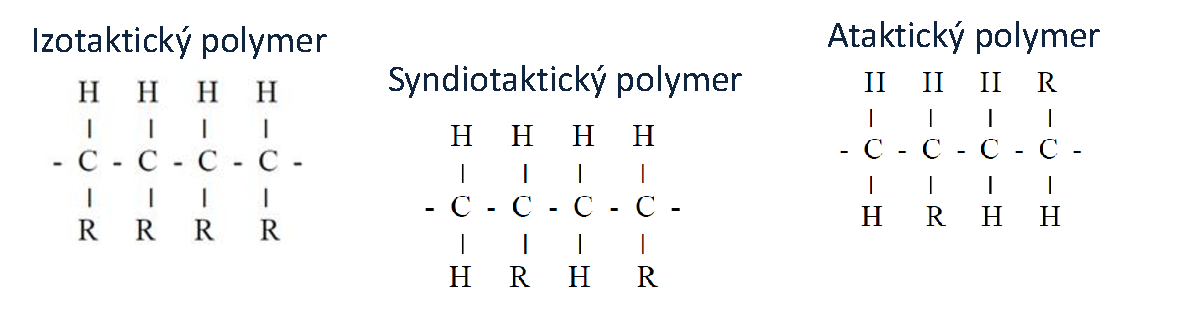
\includegraphics[width=\linewidth,height=52mm,keepaspectratio]{obrazky/emv1_p6_s06.pdf}
\par\vspace{1mm}{\scriptsize\sffamily\color{muted} Izotaktické, syndiotaktické a ataktické uspořádání. P6, s. 6.\par}
\end{minipage}
\par\end{minipage}\par\vspace{6mm}
\noindent\begin{minipage}[b]{\linewidth}
\section*{52. Popište základní tři způsoby syntézy makromolekulárních látek -- polymeraci, polyadici a polykondenzaci. V čem se jednotlivé syntézy liší?}
\begin{itemize}
\item \textbf{Polymerace:} monomery se spojují do řetězce, např. otevřením násobné vazby. Probíhá iniciace, růst a ukončení řetězce; nemění se chemické složení základní jednotky a nevzniká vedlejší nízkomolekulární produkt. Příklad: ethylen $\to$ polyethylen.
\item \textbf{Polyadice:} reagují funkční skupiny monomerů, vzniká chemicky odlišná základní jednotka, ale bez odštěpení malé molekuly. Příklad: diisokyanát a diol $\to$ polyuretan.
\item \textbf{Polykondenzace:} reakcí funkčních skupin vzniká polymer a současně se odštěpují malé molekuly, např. voda či HCl. Příklad: diamin a dikarboxylová kyselina $\to$ polyamid a voda.
\end{itemize}

\par\vspace{2mm}
\begin{minipage}[t]{.94\linewidth}\centering
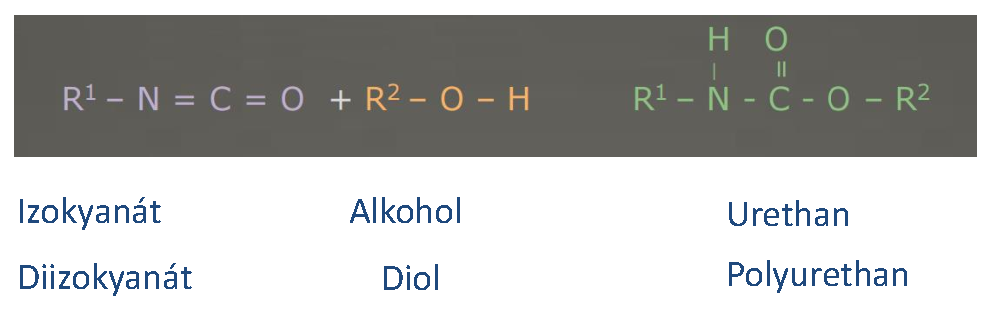
\includegraphics[width=\linewidth,height=52mm,keepaspectratio]{obrazky/emv1_p6_s16.pdf}
\par\vspace{1mm}{\scriptsize\sffamily\color{muted} Polyadiční vznik urethanové vazby. P6, s. 16.\par}
\end{minipage}
\par\end{minipage}\par\vspace{6mm}
\noindent\begin{minipage}[b]{\linewidth}
\section*{53. Jaké znáte technologické procesy polymerace a jaké mají výhody či nevýhody, popište jeden vybraný proces?}
\begin{itemize}
\item \textbf{Bloková:} polymeruje monomer s iniciátorem; velmi čistý produkt, ale obtížná regulace kvůli špatnému odvodu tepla.
\item \textbf{Suspenzní:} monomer nerozpustný ve vodě tvoří kapky, iniciátor je rozpustný v monomeru. Dobrá regulace, perličkový produkt bez zbytků emulgátoru.
\item \textbf{Emulzní:} vodné prostředí, emulgátor a iniciátor rozpustný ve vodě. Dobrá regulace, nevýhodou jsou zbytky emulgátoru a mléčné zbarvení produktu.
\item \textbf{Roztoková:} monomer i polymer jsou rozpuštěny v rozpouštědle; omezením je vznik polymerů s nižší molekulovou hmotností.
\end{itemize}
\textbf{Emulzní proces:} emulgátor vytváří micely; po zahájení polymerace vznikají a rostou polymerní částice. Výsledkem je latex. Polymer lze vysrážet přidáním elektrolytu, který neutralizuje náboj částic.

\par\vspace{2mm}
\begin{minipage}[t]{.94\linewidth}\centering
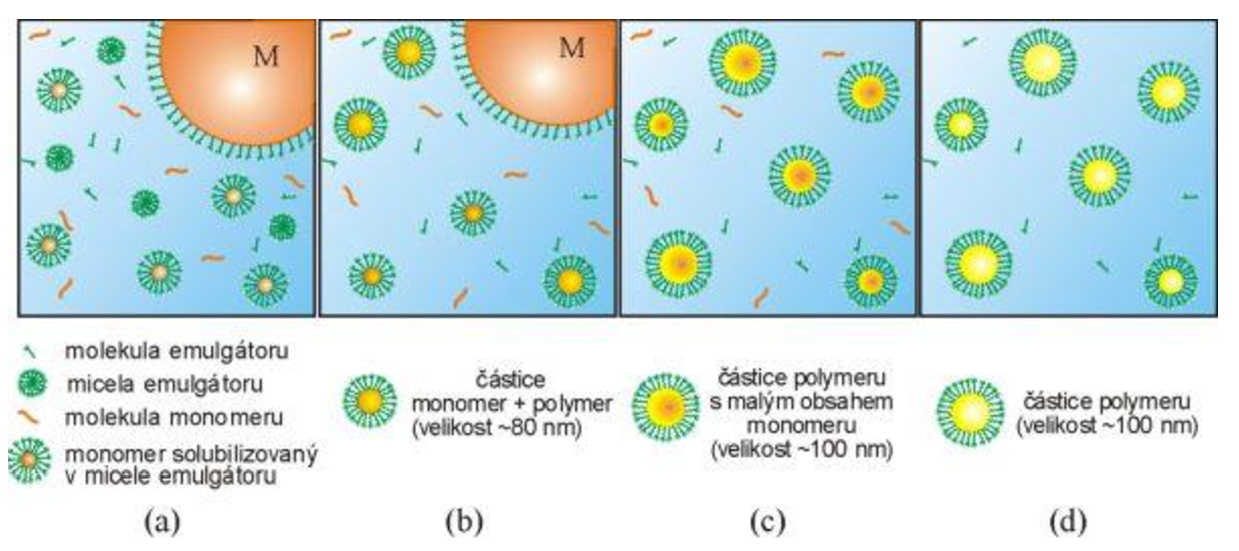
\includegraphics[width=\linewidth,height=52mm,keepaspectratio]{obrazky/emv1_p6_s15.pdf}
\par\vspace{1mm}{\scriptsize\sffamily\color{muted} Částice a jednotlivé fáze emulzní polymerace. P6, s. 15.\par}
\end{minipage}
\par\end{minipage}\par\vspace{6mm}
\noindent\begin{minipage}[b]{\linewidth}
\section*{54. Popište amorfní a semikrystalický stav organických makromolekulárních látek.}
\begin{itemize}
\item \textbf{Amorfní stav:} řetězce jsou nepravidelně stočené a propletené, bez pravidelného uspořádání; mohou vytvářet globulární útvary.
\item \textbf{Semikrystalický stav:} vedle amorfních oblastí jsou přítomny oblasti krystalické. Řetězce se pravidelně skládají do lamel, které se seskupují do sférolitů. Podíl krystalické části vyjadřuje stupeň krystalinity.
\end{itemize}

\par\vspace{2mm}
\begin{minipage}[t]{.94\linewidth}\centering
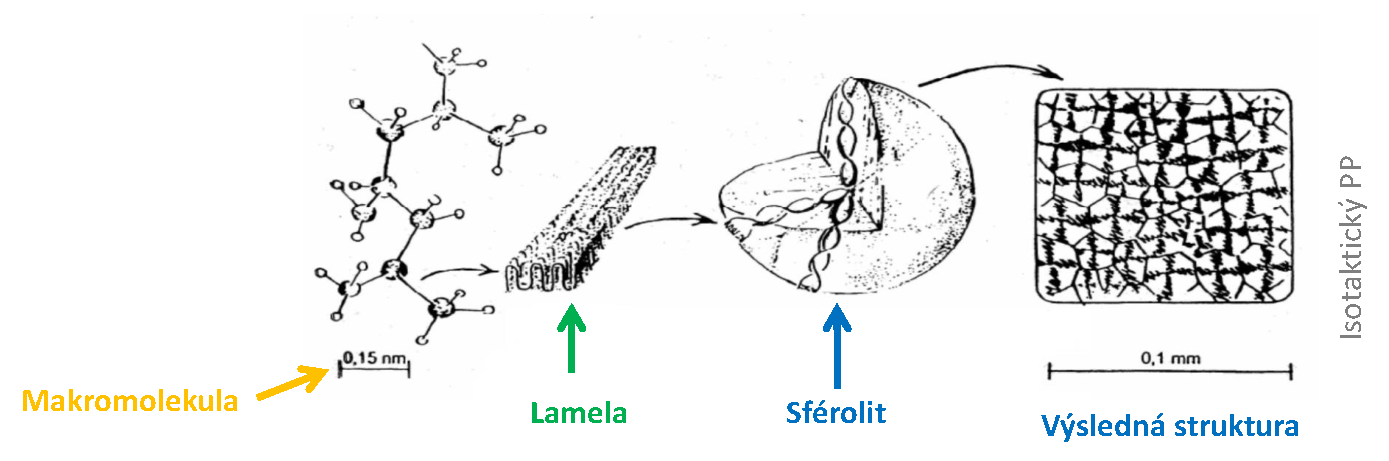
\includegraphics[width=\linewidth,height=52mm,keepaspectratio]{obrazky/emv1_p6_s08.pdf}
\par\vspace{1mm}{\scriptsize\sffamily\color{muted} Od řetězce přes lamelu a sférolit ke struktuře polymeru. P6, s. 8.\par}
\end{minipage}
\par\end{minipage}\par\vspace{6mm}
\noindent\begin{minipage}[b]{\linewidth}
\section*{55. Uveďte čtyři zástupce ze skupiny termoplastů a tři ze skupiny reaktoplastů a detailněji popište vlastnosti jednoho zástupce z každé kategorie.}
\textbf{Čtyři termoplasty:} PE, PP, PVC, PS. \textbf{Tři reaktoplasty:} fenoplasty PF, epoxidové pryskyřice EP, melaminoformaldehydové pryskyřice MF.
\begin{itemize}
\item \textbf{Polyethylen (PE):} nepolární semikrystalický polymer, lehký, chemicky odolný a málo nasákavý. Vysokotlaký PE má nižší hustotu a měkne kolem $105\,^{\circ}\mathrm C$, nízkotlaký je hustší a měkne kolem $130\,^{\circ}\mathrm C$. Je výborný izolant: $\varepsilon_r\approx2{,}25$--$2{,}30$, $\tan\delta\approx(1$--$3)\cdot10^{-4}$, $\rho_V\sim10^{15}\,\Omega\,\mathrm m$. Používá se na kabelové izolace včetně vf techniky.
\item \textbf{Epoxidové pryskyřice (EP):} vytvrzením vzniká prostorová síť. Mají dobrou přilnavost ke kovům, keramice a sklu, malou nasákavost a dobré elektrické vlastnosti: $\varepsilon_r\approx4$, $\tan\delta\sim10^{-3}$ při 100 Hz. Přednáška uvádí dlouhodobou tepelnou odolnost asi $160\,^{\circ}\mathrm C$. Použití: zalévací hmoty, lepidla a lamináty FR-4.
\end{itemize}

\par\end{minipage}\par\vspace{6mm}
\noindent\begin{minipage}[b]{\linewidth}
\section*{56. Jak lze zvýšit stabilitu plastů? Jmenujte zástupce plastů se zvýšenou tepelnou odolností.}
Stabilitu plastů lze zvýšit:
\begin{itemize}
\item přidáním tepelných stabilizátorů, antioxidantů a UV absorbérů;
\item zvýšením krystalinity a tuhosti řetězců, např. začleněním aromatických kruhů;
\item použitím odolnějších vazeb: náhradou C--H za C--F nebo páteří Si--O;
\item použitím výztužných materiálů.
\end{itemize}
\textbf{Plasty se zvýšenou tepelnou odolností:} polyfenylenoxid PPO, polysulfon PSU, polyethersulfon PES, polyfenylensulfid PPS, polyimidy PI, polyetheretherketon PEEK a silikony.

\par\vspace{2mm}
\begin{minipage}[t]{.94\linewidth}\centering
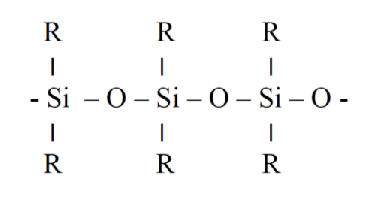
\includegraphics[width=\linewidth,height=52mm,keepaspectratio]{obrazky/emv1_p6_s32.pdf}
\par\vspace{1mm}{\scriptsize\sffamily\color{muted} Páteřní řetězec silikonů s vazbami Si--O. P6, s. 32.\par}
\end{minipage}
\par\end{minipage}\par\vspace{6mm}
\noindent\begin{minipage}[b]{\linewidth}
\section*{57. Popište proces výroby pryže a vysvětlete pojem vulkanizace.}
\begin{enumerate}
\item \textbf{Získání kaučuku:} přírodní kaučuk se oddělí z latexu odpařením vody nebo koagulací kyselinou; lze použít také syntetický kaučuk.
\item \textbf{Příprava směsi:} přidají se plniva a vulkanizační činidlo. Hnětení částečně zkracuje řetězce a zvyšuje zpracovatelnost kaučuku.
\item \textbf{Vulkanizace:} při zahřívání se mezi řetězci vytvářejí příčné chemické vazby. Při vulkanizaci sírou vznikají sirné můstky, obvykle při $140$--$150\,^{\circ}\mathrm C$.
\end{enumerate}
Z kaučuku vzniká pružná \textbf{pryž}; množství síry a míra zesítění určují její tvrdost.

\par\vspace{2mm}
\begin{minipage}[t]{.94\linewidth}\centering
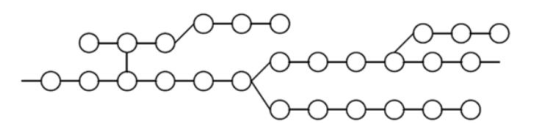
\includegraphics[width=\linewidth,height=52mm,keepaspectratio]{obrazky/emv1_p6_s07.pdf}
\par\vspace{1mm}{\scriptsize\sffamily\color{muted} Příčné propojení makromolekulárních řetězců. P6, s. 7.\par}
\end{minipage}
\par\end{minipage}\par\vspace{6mm}
\noindent\begin{minipage}[b]{\linewidth}
\section*{58. Popište dia-, para- a feromagnetismus a jak se tyto látky projevují po vložení do magnetického pole?}
\begin{itemize}
\item \textbf{Diamagnetismus:} bez pole mají atomy nulový výsledný magnetický moment. Pole vyvolá malý moment opačného směru, takže magnetická indukce je menší než ve vakuu; $\chi_m<0$, $\mu_r<1$. Příklady: Cu, Ag, voda.
\item \textbf{Paramagnetismus:} atomy mají nenulové momenty, které jsou bez pole neuspořádané. V poli se částečně orientují souhlasně, takže indukce vzroste; $\chi_m>0$, $\mu_r>1$. Příklady: Al, Pt, O$_2$.
\item \textbf{Feromagnetismus:} existují spontánně zmagnetované domény. Vnější pole mění jejich velikost a orientaci, vzniká silná magnetizace s nasycením a hysterezí; po odstranění pole může zůstat remanence. Příklady: Fe, Co, Ni.
\end{itemize}

\par\vspace{2mm}
\begin{minipage}[t]{.48\linewidth}\centering
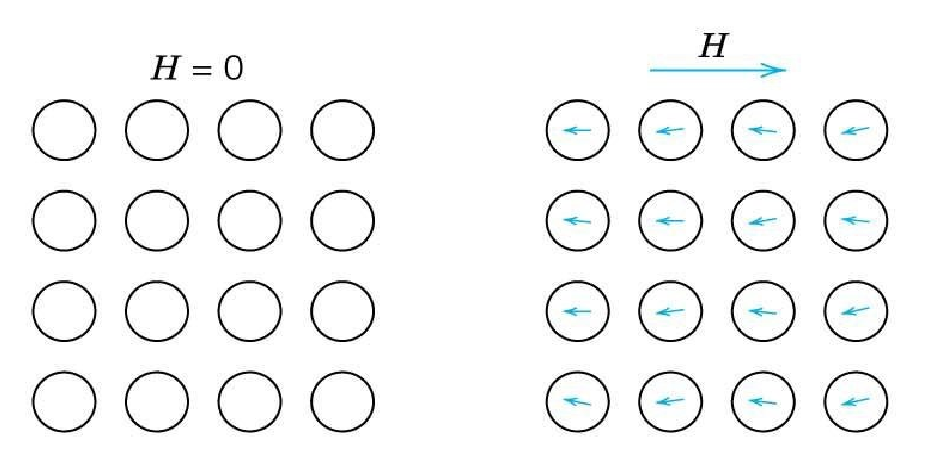
\includegraphics[width=\linewidth,height=52mm,keepaspectratio]{obrazky/emv1_p7_s11.pdf}
\par\vspace{1mm}{\scriptsize\sffamily\color{muted} Diamagnetická odezva proti působícímu poli. P7, s. 11.\par}
\end{minipage}\hfill
\begin{minipage}[t]{.48\linewidth}\centering
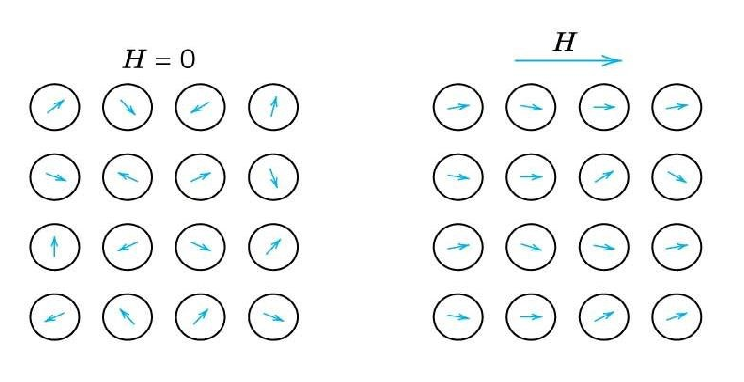
\includegraphics[width=\linewidth,height=52mm,keepaspectratio]{obrazky/emv1_p7_s13.pdf}
\par\vspace{1mm}{\scriptsize\sffamily\color{muted} Částečné souhlasné uspořádání paramagnetických momentů. P7, s. 13.\par}
\end{minipage}
\par\end{minipage}\par\vspace{6mm}
\noindent\begin{minipage}[b]{\linewidth}
\section*{59. Jaká je podstata vzniku feromagnetika a jaké jsou rozdíly mezi fero-, antifero- a ferimagnetika.}
Feromagnetismus vyžaduje \textbf{nevykompenzované magnetické momenty atomů}, zejména spiny elektronů v neúplně obsazených vnitřních hladinách, a \textbf{výměnné síly} mezi sousedními atomy. Ty zajišťují spontánní uspořádání momentů v doménách.
\begin{itemize}
\item \textbf{Fero-:} momenty jsou souhlasně orientované, výsledná spontánní magnetizace je nenulová; Fe, Co, Ni.
\item \textbf{Antifero-:} podmřížky mají opačně orientované, stejně velké magnetizace, které se vyruší; např. MnO.
\item \textbf{Feri-:} podmřížky mají opačně orientované, ale nestejně velké magnetizace, takže se nevyruší; např. magnetit Fe$_3$O$_4$.
\end{itemize}

\par\vspace{2mm}
\begin{minipage}[t]{.94\linewidth}\centering
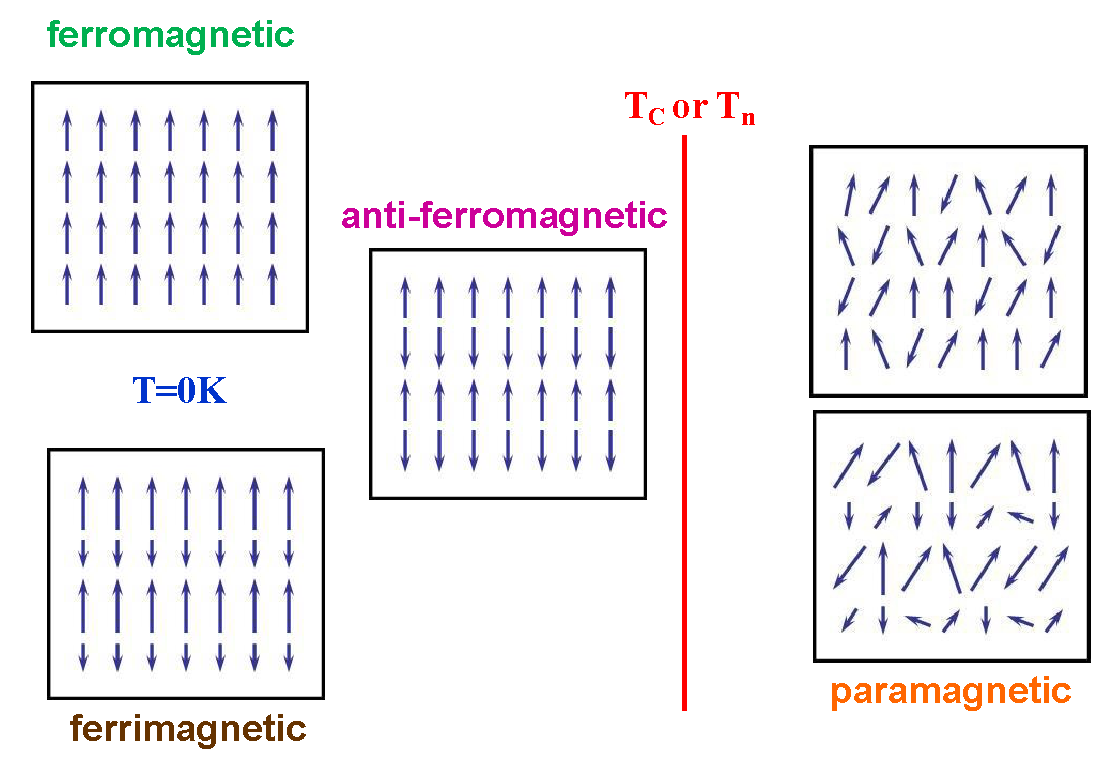
\includegraphics[width=\linewidth,height=52mm,keepaspectratio]{obrazky/emv1_p7_s64.pdf}
\par\vspace{1mm}{\scriptsize\sffamily\color{muted} Uspořádání momentů a teplotní zánik uspořádaného stavu. P7, s. 64.\par}
\end{minipage}
\par\end{minipage}\par\vspace{6mm}
\noindent\begin{minipage}[b]{\linewidth}
\section*{60. Nakreslete křivku prvotní magnetizace a popište jednotlivé fáze křivky s ohledem na děje v materiálu.}
Křivka prvotní magnetizace $M(H)$ začíná v odmagnetovaném stavu a má čtyři oblasti:
\begin{enumerate}
\item \textbf{I: vratné posuny Blochových stěn}; domény orientované výhodně vůči poli se zvětšují, magnetizace roste mírně.
\item \textbf{II: nevratné posuny stěn}; výhodně orientované domény rostou na úkor ostatních, magnetizace roste strmě.
\item \textbf{III: stáčení vektoru spontánní magnetizace} do směru vnějšího pole.
\item \textbf{IV: nasycení a paraproces}; směr magnetizace se již nemění, její velikost při dalším zesilování pole jen nepatrně roste.
\end{enumerate}

\par\vspace{2mm}
\begin{minipage}[t]{.94\linewidth}\centering
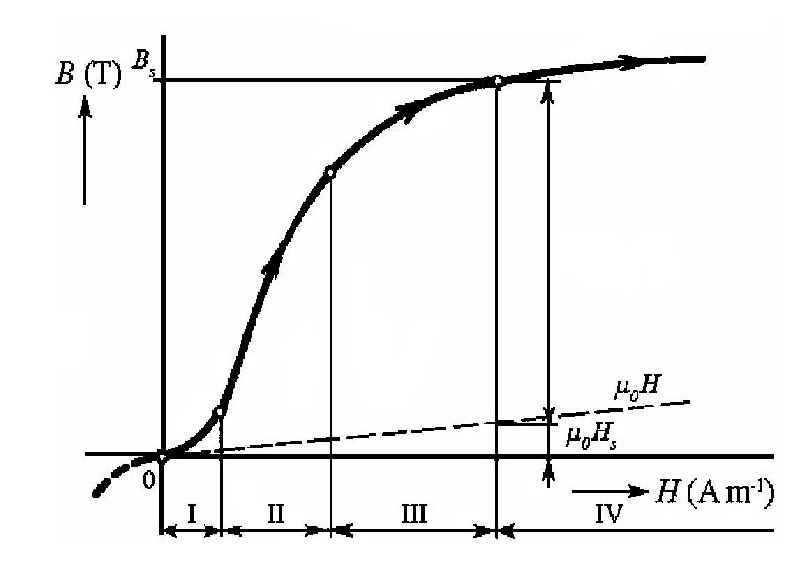
\includegraphics[width=\linewidth,height=52mm,keepaspectratio]{obrazky/emv1_p7_s37.pdf}
\par\vspace{1mm}{\scriptsize\sffamily\color{muted} Čtyři oblasti prvotní magnetizace. P7, s. 37.\par}
\end{minipage}
\par\end{minipage}\par\vspace{6mm}
\noindent\begin{minipage}[b]{\linewidth}
\section*{61. Nakreslete a popište hysterezní smyčku a uveďte čím se liší od magnetizační smyčky.}
\textbf{Hysterezní smyčka} vzniká při cyklické změně pole; magnetický stav závisí i na předchozím magnetování.
\begin{itemize}
\item Z nasycení při poklesu na $H=0$ zbývá \textbf{remanence} $B_r$ nebo $M_r$.
\item Opačné \textbf{koercitivní pole} $-H_c$ zruší příslušnou indukci či magnetizaci; silnější opačné pole vytvoří záporné nasycení.
\item Zpětná větev přes zápornou remanenci a kladnou koercivitu uzavírá smyčku.
\end{itemize}
\textbf{Křivka prvotní magnetizace} naproti tomu není uzavřená: vede z odmagnetovaného počátku k nasycení při postupném zvyšování pole. Hysterezní smyčka popisuje celý cyklus přemagnetování.

\par\vspace{2mm}
\begin{minipage}[t]{.94\linewidth}\centering
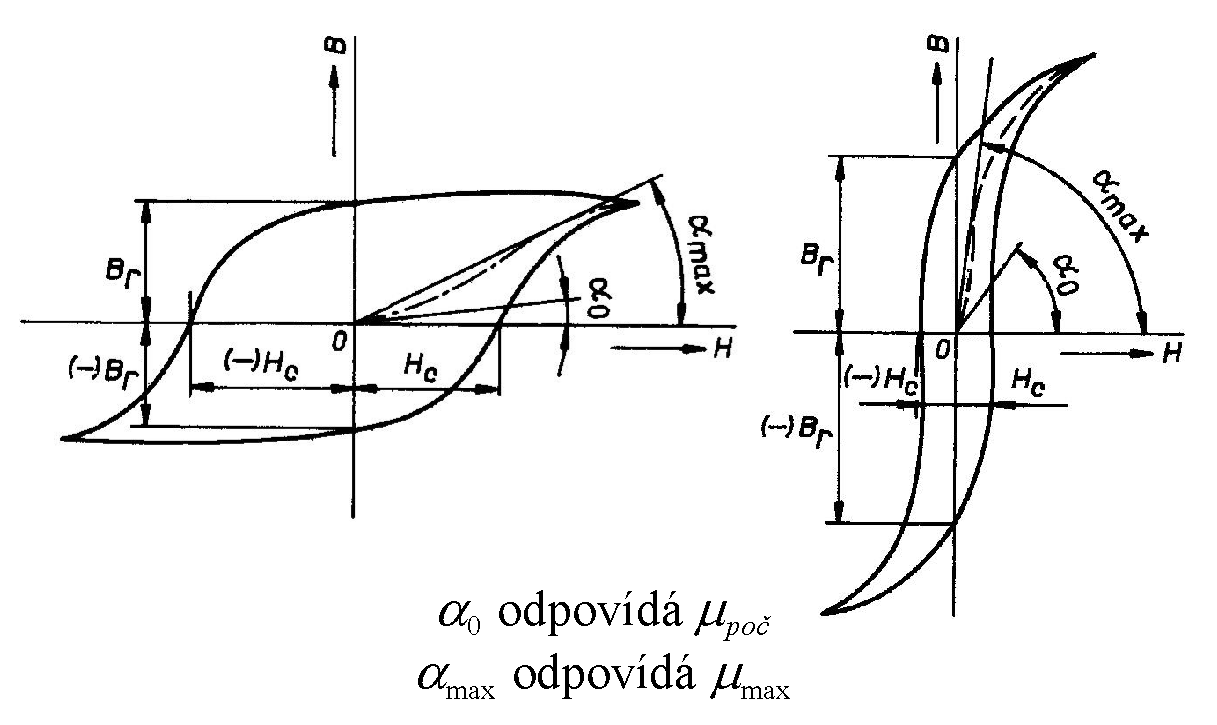
\includegraphics[width=\linewidth,height=52mm,keepaspectratio]{obrazky/emv1_p7_s39.pdf}
\par\vspace{1mm}{\scriptsize\sffamily\color{muted} Smyčky magneticky tvrdého a měkkého materiálu. P7, s. 39.\par}
\end{minipage}
\par\end{minipage}\par\vspace{6mm}
\noindent\begin{minipage}[b]{\linewidth}
\section*{62. Co je to komutační křivka a dynamická hysterezní smyčka a k čemu se používají?}
\begin{itemize}
\item \textbf{Komutační křivka:} spojnice vrcholů ustálených souměrných hysterezních smyček získaných při různých amplitudách pole. Téměř se shoduje s křivkou prvotní magnetizace, ale snáze a přesněji se měří, proto ji v praxi zastupuje.
\item \textbf{Dynamická hysterezní smyčka:} smyčka při rychlých změnách střídavého pole. S frekvencí se oproti statické smyčce rozšiřuje, její špičky se zaoblují a roste koercitivní pole; závisí i na časovém průběhu indukce. Používá se k posouzení magnetování a ztrát při střídavém provozu.
\end{itemize}

\par\vspace{2mm}
\begin{minipage}[t]{.48\linewidth}\centering
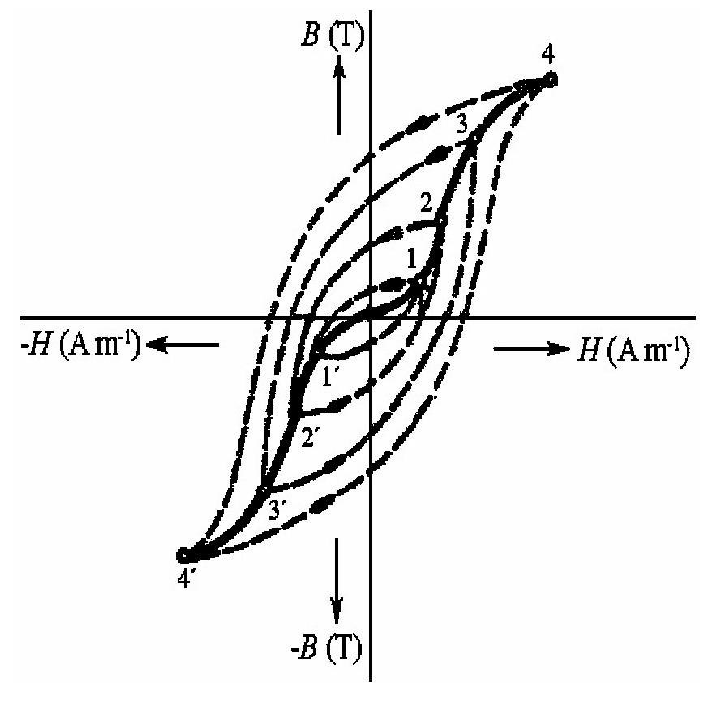
\includegraphics[width=\linewidth,height=52mm,keepaspectratio]{obrazky/emv1_p7_s42.pdf}
\par\vspace{1mm}{\scriptsize\sffamily\color{muted} Komutační křivka spojující vrcholy smyček. P7, s. 42.\par}
\end{minipage}\hfill
\begin{minipage}[t]{.48\linewidth}\centering
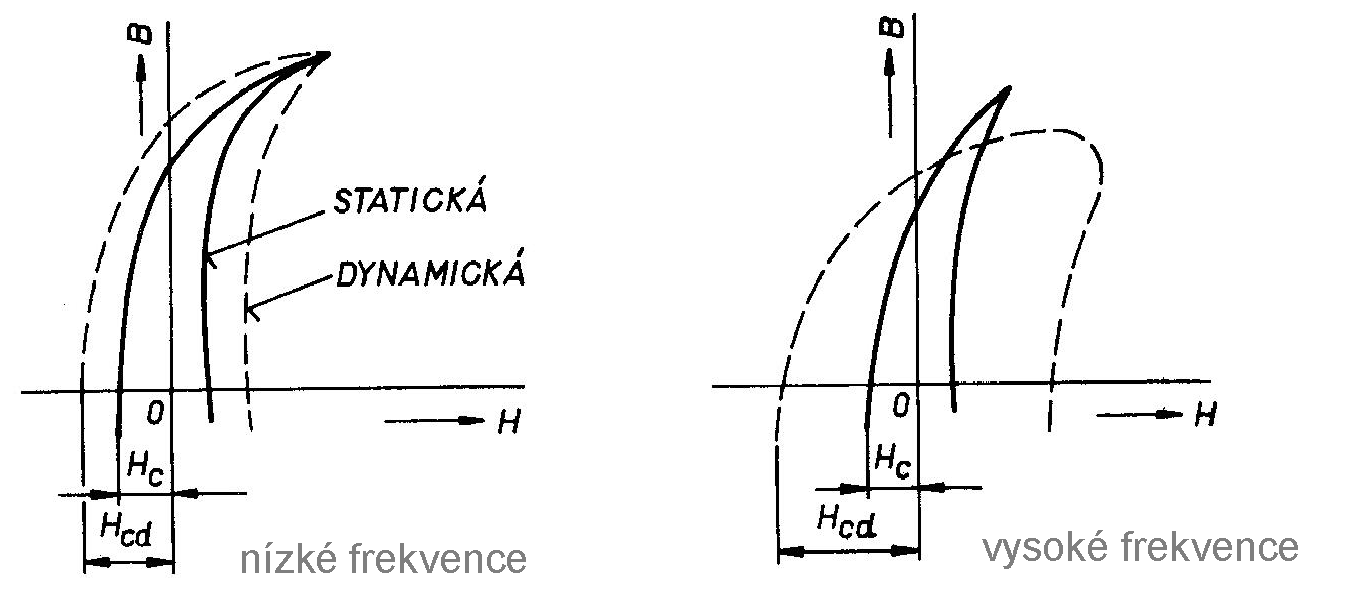
\includegraphics[width=\linewidth,height=52mm,keepaspectratio]{obrazky/emv1_p7_s48.pdf}
\par\vspace{1mm}{\scriptsize\sffamily\color{muted} Statická a dynamická smyčka při různých frekvencích. P7, s. 48.\par}
\end{minipage}
\par\end{minipage}\par\vspace{6mm}
\noindent\begin{minipage}[b]{\linewidth}
\section*{63. Jaká teplota shora omezuje tzv. feromagnetický stav a jakým jiným způsobem lze docílit „odmagnetování“?}
Horní mez feromagnetického stavu určuje \textbf{Curieova teplota $T_C$}; nad ní zaniká spontánní uspořádání a látka přechází do paramagnetického stavu.

Jiným způsobem odmagnetování je \textbf{střídavé magnetické pole s postupně klesající amplitudou až k nule}. Zmenšující se hysterezní smyčky vedou k odmagnetovanému stavu.

\par\vspace{2mm}
\begin{minipage}[t]{.94\linewidth}\centering
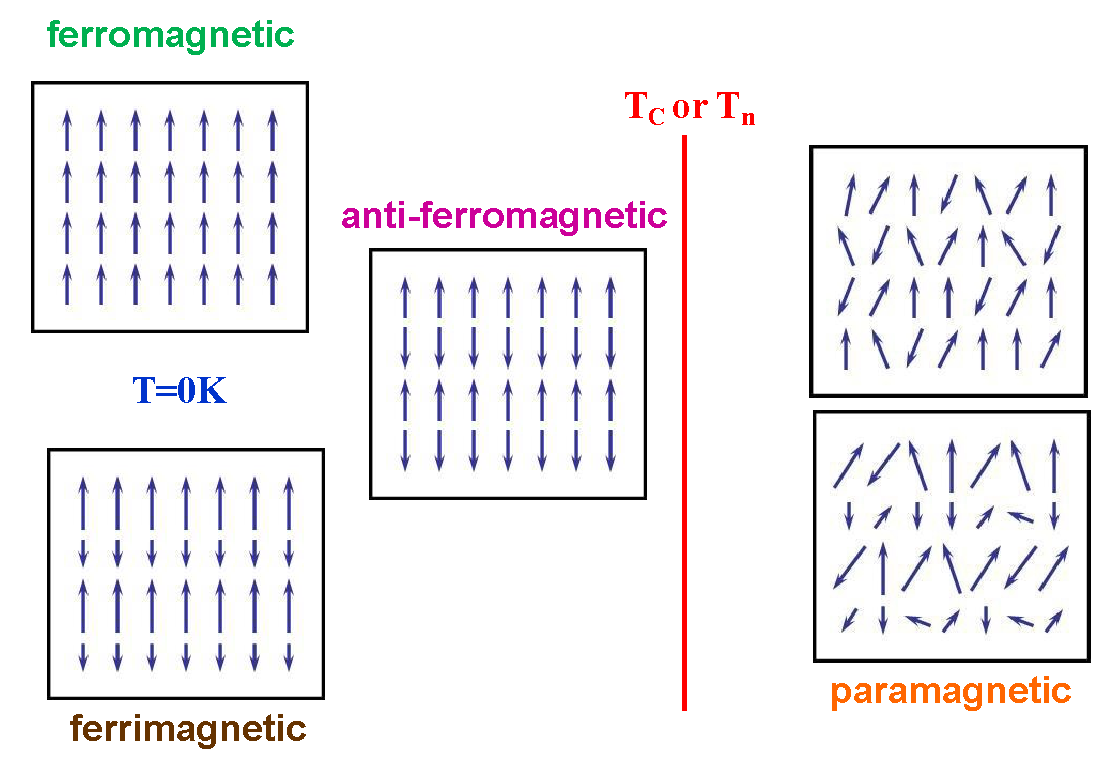
\includegraphics[width=\linewidth,height=52mm,keepaspectratio]{obrazky/emv1_p7_s64.pdf}
\par\vspace{1mm}{\scriptsize\sffamily\color{muted} Uspořádání momentů a teplotní zánik uspořádaného stavu. P7, s. 64.\par}
\end{minipage}
\par\end{minipage}\par\vspace{6mm}
\noindent\begin{minipage}[b]{\linewidth}
\section*{64. Jmenujte významné magneticky měkké a magneticky tvrdé materiály a v jakých aplikacích je lze použít.}
\textbf{Magneticky měkké materiály} mají malou koercivitu a úzkou hysterezní smyčku:
\begin{itemize}
\item technicky čisté Fe -- stejnosměrné magnetické obvody;
\item Fe--Si plechy -- transformátory a elektrické stroje;
\item Fe--Ni slitiny (permalloy, supermalloy, mumetal) -- jádra transformátorů a tlumivek, magnetické stínění;
\item sendust (Fe--Al--Si) a měkké ferity -- magnetická jádra cívek a tlumivek.
\end{itemize}
\textbf{Magneticky tvrdé materiály} mají velkou koercivitu a širokou smyčku. Patří sem oceli legované W, Cr či Co, slitiny AlNi, AlNiCo, CuNiFe a CuNiCo; používají se pro \textbf{permanentní magnety}.

\par\vspace{2mm}
\begin{minipage}[t]{.94\linewidth}\centering
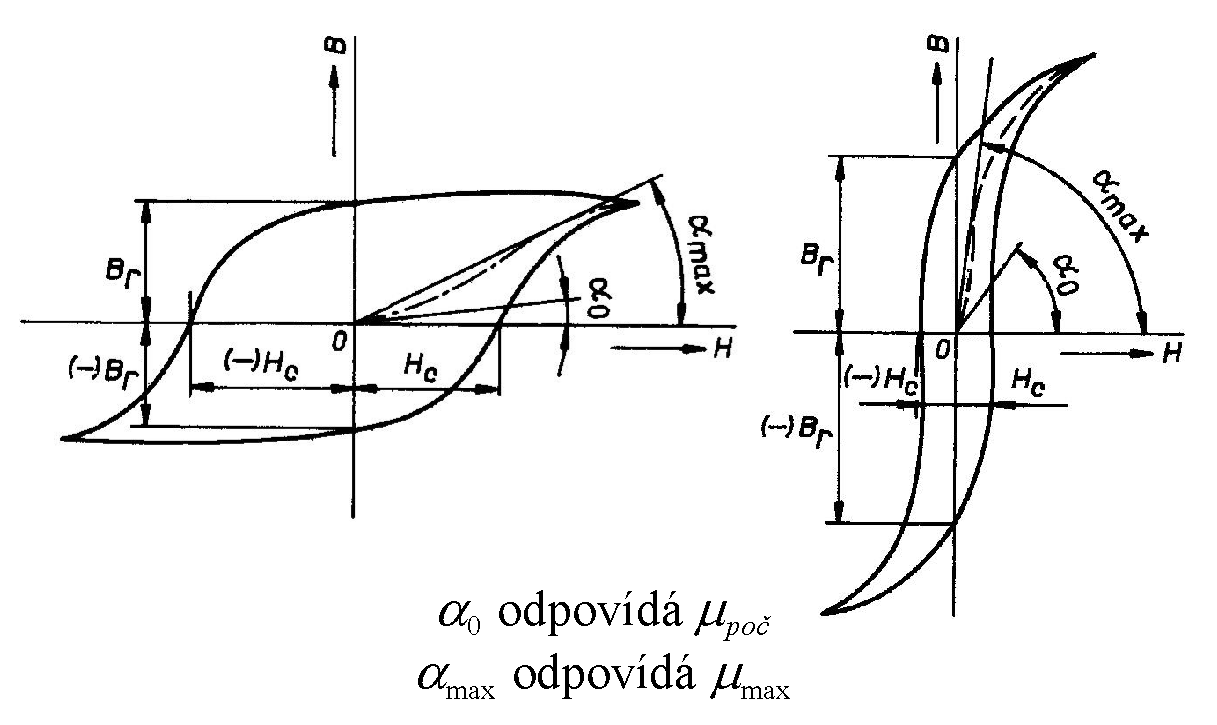
\includegraphics[width=\linewidth,height=52mm,keepaspectratio]{obrazky/emv1_p7_s39.pdf}
\par\vspace{1mm}{\scriptsize\sffamily\color{muted} Smyčky magneticky tvrdého a měkkého materiálu. P7, s. 39.\par}
\end{minipage}
\par\end{minipage}\par\vspace{6mm}
\noindent\begin{minipage}[b]{\linewidth}
\section*{65. Jaké znáte typy ztrát v magnetických materiálech a jaká je jejich závislost na kmitočtu magnetického pole.}
Celkové ztráty při přemagnetování jsou $P=P_h+P_v+P_z$:
\begin{itemize}
\item \textbf{Hysterezní $P_h$:} souvisejí se změnami domén; $P_h=VS_hf$, tedy při stejné smyčce rostou \textbf{lineárně s frekvencí}. $V$ je objem a $S_h$ plocha statické smyčky.
\item \textbf{Vířivými proudy $P_v$:} indukované proudy ohřívají elektricky vodivé jádro. Při stejné geometrii, rezistivitě a amplitudě indukce platí \textbf{$P_v\propto f^2$}.
\item \textbf{Magnetickým zpožděním $P_z$:} souvisejí s pohyby elektronů v mřížce při změnách pole; významné jsou u feritů a v malých polích u měkkých materiálů. Přednáška pro ně konkrétní kmitočtovou závislost neuvádí.
\end{itemize}

\par\vspace{2mm}
\begin{minipage}[t]{.94\linewidth}\centering
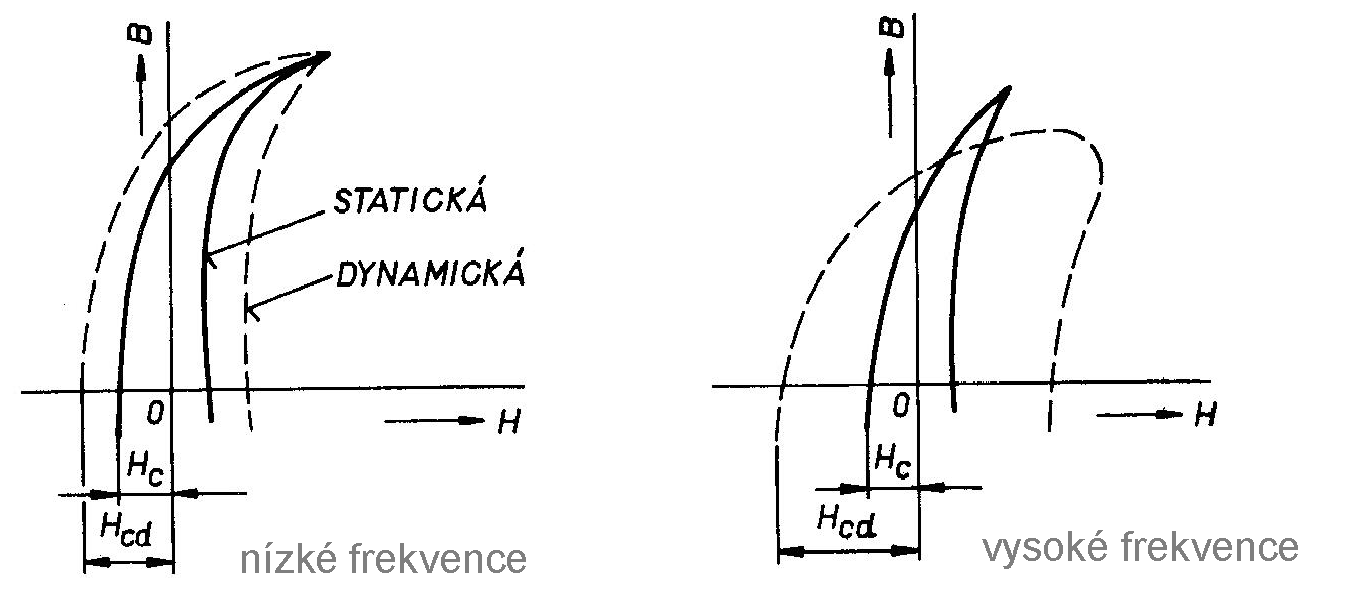
\includegraphics[width=\linewidth,height=52mm,keepaspectratio]{obrazky/emv1_p7_s48.pdf}
\par\vspace{1mm}{\scriptsize\sffamily\color{muted} Statická a dynamická smyčka při různých frekvencích. P7, s. 48.\par}
\end{minipage}
\par\end{minipage}\par\vspace{6mm}
\noindent\begin{minipage}[b]{\linewidth}
\section*{66. Jaké znáte zástupce feritů a stručně popište jejich vlastnosti.}
\textbf{Ferity} jsou sloučeniny oxidu železa s oxidy dalších kovů. Mají malou elektrickou vodivost, a tím malé ztráty vířivými proudy; jsou tvrdé, křehké, chemicky netečné a nenavlhají.
\begin{itemize}
\item \textbf{Spinelové ferity} $\mathrm{MO\cdot Fe_2O_3}$: magnetit $\mathrm{FeO\cdot Fe_2O_3}$, nikelnatý a kobaltnatý ferit. Jejich vlastnosti závisejí na obsazení podmřížek; normální struktury (např. Zn a Cd ferit) nemají ferimagnetické uspořádání, inverzní je mají.
\item \textbf{Smíšené ferity Mn--Zn, Ni--Zn, Cu--Zn:} kombinují oxidy více kovů; díky lepším magnetickým vlastnostem patří k nejpoužívanějším.
\item \textbf{Ferity typu magnetoplumbitu:} šesterečná struktura, např. $\mathrm{PbO\cdot6Fe_2O_3}$; také ferity s Ba či Sr.
\item \textbf{Granátové ferity:} obsahují prvky jako Y, Gd nebo Sc, mají granátovou strukturu se třemi podmřížkami.
\end{itemize}

\par\vspace{2mm}
\begin{minipage}[t]{.94\linewidth}\centering
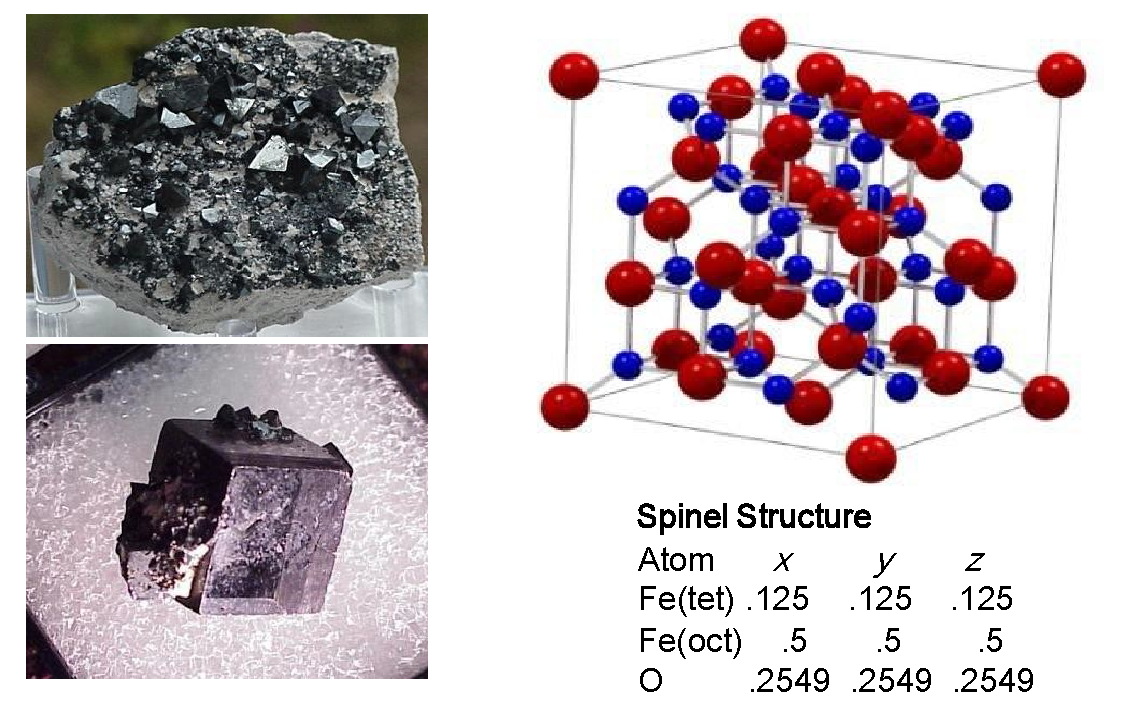
\includegraphics[width=\linewidth,height=52mm,keepaspectratio]{obrazky/emv1_p7_s62.pdf}
\par\vspace{1mm}{\scriptsize\sffamily\color{muted} Magnetit a jeho spinelová struktura. P7, s. 62.\par}
\end{minipage}
\par\end{minipage}\par\vspace{6mm}
\end{document}
